\PassOptionsToPackage{unicode=true}{hyperref} % options for packages loaded elsewhere
\PassOptionsToPackage{hyphens}{url}
%
\documentclass[]{book}
\usepackage{lmodern}
\usepackage{amssymb,amsmath}
\usepackage{ifxetex,ifluatex}
\usepackage{fixltx2e} % provides \textsubscript
\ifnum 0\ifxetex 1\fi\ifluatex 1\fi=0 % if pdftex
  \usepackage[T1]{fontenc}
  \usepackage[utf8]{inputenc}
  \usepackage{textcomp} % provides euro and other symbols
\else % if luatex or xelatex
  \usepackage{unicode-math}
  \defaultfontfeatures{Ligatures=TeX,Scale=MatchLowercase}
\fi
% use upquote if available, for straight quotes in verbatim environments
\IfFileExists{upquote.sty}{\usepackage{upquote}}{}
% use microtype if available
\IfFileExists{microtype.sty}{%
\usepackage[]{microtype}
\UseMicrotypeSet[protrusion]{basicmath} % disable protrusion for tt fonts
}{}
\IfFileExists{parskip.sty}{%
\usepackage{parskip}
}{% else
\setlength{\parindent}{0pt}
\setlength{\parskip}{6pt plus 2pt minus 1pt}
}
\usepackage{hyperref}
\hypersetup{
            pdftitle={语言数据科学教程},
            pdfauthor={陈居强},
            pdfborder={0 0 0},
            breaklinks=true}
\urlstyle{same}  % don't use monospace font for urls
\usepackage{color}
\usepackage{fancyvrb}
\newcommand{\VerbBar}{|}
\newcommand{\VERB}{\Verb[commandchars=\\\{\}]}
\DefineVerbatimEnvironment{Highlighting}{Verbatim}{commandchars=\\\{\}}
% Add ',fontsize=\small' for more characters per line
\usepackage{framed}
\definecolor{shadecolor}{RGB}{248,248,248}
\newenvironment{Shaded}{\begin{snugshade}}{\end{snugshade}}
\newcommand{\AlertTok}[1]{\textcolor[rgb]{0.94,0.16,0.16}{#1}}
\newcommand{\AnnotationTok}[1]{\textcolor[rgb]{0.56,0.35,0.01}{\textbf{\textit{#1}}}}
\newcommand{\AttributeTok}[1]{\textcolor[rgb]{0.77,0.63,0.00}{#1}}
\newcommand{\BaseNTok}[1]{\textcolor[rgb]{0.00,0.00,0.81}{#1}}
\newcommand{\BuiltInTok}[1]{#1}
\newcommand{\CharTok}[1]{\textcolor[rgb]{0.31,0.60,0.02}{#1}}
\newcommand{\CommentTok}[1]{\textcolor[rgb]{0.56,0.35,0.01}{\textit{#1}}}
\newcommand{\CommentVarTok}[1]{\textcolor[rgb]{0.56,0.35,0.01}{\textbf{\textit{#1}}}}
\newcommand{\ConstantTok}[1]{\textcolor[rgb]{0.00,0.00,0.00}{#1}}
\newcommand{\ControlFlowTok}[1]{\textcolor[rgb]{0.13,0.29,0.53}{\textbf{#1}}}
\newcommand{\DataTypeTok}[1]{\textcolor[rgb]{0.13,0.29,0.53}{#1}}
\newcommand{\DecValTok}[1]{\textcolor[rgb]{0.00,0.00,0.81}{#1}}
\newcommand{\DocumentationTok}[1]{\textcolor[rgb]{0.56,0.35,0.01}{\textbf{\textit{#1}}}}
\newcommand{\ErrorTok}[1]{\textcolor[rgb]{0.64,0.00,0.00}{\textbf{#1}}}
\newcommand{\ExtensionTok}[1]{#1}
\newcommand{\FloatTok}[1]{\textcolor[rgb]{0.00,0.00,0.81}{#1}}
\newcommand{\FunctionTok}[1]{\textcolor[rgb]{0.00,0.00,0.00}{#1}}
\newcommand{\ImportTok}[1]{#1}
\newcommand{\InformationTok}[1]{\textcolor[rgb]{0.56,0.35,0.01}{\textbf{\textit{#1}}}}
\newcommand{\KeywordTok}[1]{\textcolor[rgb]{0.13,0.29,0.53}{\textbf{#1}}}
\newcommand{\NormalTok}[1]{#1}
\newcommand{\OperatorTok}[1]{\textcolor[rgb]{0.81,0.36,0.00}{\textbf{#1}}}
\newcommand{\OtherTok}[1]{\textcolor[rgb]{0.56,0.35,0.01}{#1}}
\newcommand{\PreprocessorTok}[1]{\textcolor[rgb]{0.56,0.35,0.01}{\textit{#1}}}
\newcommand{\RegionMarkerTok}[1]{#1}
\newcommand{\SpecialCharTok}[1]{\textcolor[rgb]{0.00,0.00,0.00}{#1}}
\newcommand{\SpecialStringTok}[1]{\textcolor[rgb]{0.31,0.60,0.02}{#1}}
\newcommand{\StringTok}[1]{\textcolor[rgb]{0.31,0.60,0.02}{#1}}
\newcommand{\VariableTok}[1]{\textcolor[rgb]{0.00,0.00,0.00}{#1}}
\newcommand{\VerbatimStringTok}[1]{\textcolor[rgb]{0.31,0.60,0.02}{#1}}
\newcommand{\WarningTok}[1]{\textcolor[rgb]{0.56,0.35,0.01}{\textbf{\textit{#1}}}}
\usepackage{longtable,booktabs}
% Fix footnotes in tables (requires footnote package)
\IfFileExists{footnote.sty}{\usepackage{footnote}\makesavenoteenv{longtable}}{}
\usepackage{graphicx,grffile}
\makeatletter
\def\maxwidth{\ifdim\Gin@nat@width>\linewidth\linewidth\else\Gin@nat@width\fi}
\def\maxheight{\ifdim\Gin@nat@height>\textheight\textheight\else\Gin@nat@height\fi}
\makeatother
% Scale images if necessary, so that they will not overflow the page
% margins by default, and it is still possible to overwrite the defaults
% using explicit options in \includegraphics[width, height, ...]{}
\setkeys{Gin}{width=\maxwidth,height=\maxheight,keepaspectratio}
\setlength{\emergencystretch}{3em}  % prevent overfull lines
\providecommand{\tightlist}{%
  \setlength{\itemsep}{0pt}\setlength{\parskip}{0pt}}
\setcounter{secnumdepth}{5}
% Redefines (sub)paragraphs to behave more like sections
\ifx\paragraph\undefined\else
\let\oldparagraph\paragraph
\renewcommand{\paragraph}[1]{\oldparagraph{#1}\mbox{}}
\fi
\ifx\subparagraph\undefined\else
\let\oldsubparagraph\subparagraph
\renewcommand{\subparagraph}[1]{\oldsubparagraph{#1}\mbox{}}
\fi

% set default figure placement to htbp
\makeatletter
\def\fps@figure{htbp}
\makeatother

\usepackage{booktabs}
\usepackage{amsthm}
\makeatletter
\def\thm@space@setup{%
  \thm@preskip=8pt plus 2pt minus 4pt
  \thm@postskip=\thm@preskip
}
\makeatother
\usepackage[]{natbib}
\bibliographystyle{apalike}

\title{语言数据科学教程}
\author{陈居强}
\date{2023-11-03}

\begin{document}
\maketitle

{
\setcounter{tocdepth}{1}
\tableofcontents
}
\hypertarget{ux7b2cux4e00ux7ae0-ux7eeaux8bba}{%
\chapter{第一章 绪论}\label{ux7b2cux4e00ux7ae0-ux7eeaux8bba}}



\hypertarget{ux6570ux636eux4e0eux6570ux636eux79d1ux5b66}{%
\section{数据与数据科学}\label{ux6570ux636eux4e0eux6570ux636eux79d1ux5b66}}

我们的生活中都充满了数据。不管是否意识到,我们每时每刻都在产生数据。

比如,早上起床时,看一眼运动手环上昨晚的睡眠时间,同时看一下这一周的睡眠趋势图。这个简单的过程就包括了数据收集,数据整理和可视化。如果你的健康设备,结合你的睡眠及身体机能指标,给你打分并提出健康建议,那就还涉及到模型建立和预测。

随着科技发展,移动终端使得我们的数据收集能力得到极大提升,我们的出行轨迹、身体状况、消费活动、音乐喜好,社交网络等等都被记录下来,并且存储在日益庞大的存储系统中。这样的海量数据已经超过了传统统计学和计算机科学的处理能力,为数据的利用带来了巨大的发展机遇与挑战。商业领域和研究领域对于数据分析有了更高的需求和期待。数据科学作为一门融合了统计学、计算机编程和专业知识的新兴学科应运而生。

数据科学是一门综合性学科,旨在通过对大量数据进行分析和挖掘,揭示数据背后的规律和趋势,为实现商业或者科研目标提供支持。数据科学在各个领域都有着广泛的应用,如金融、医疗、互联网、工业等。例如,在商业领域,数据科学可以帮助企业进行市场分析、客户行为预测和营销策略制定等工作,从而提高企业的经济效益。在医疗领域,数据科学可以帮助医生进行病例分析和诊断,提高医疗水平和效率。在政府领域,数据科学可以帮助政府进行决策和政策制定,提高政府管理水平和公共服务水平。通过数据科学的技术手段和方法,我们可以更好地理解和利用数据,从而促进社会和经济的发展。

然而,数据科学也面临着一些挑战。首先,数据质量是影响数据科学研究与应用成败的关键。如果数据质量不好或者数据不完整,将会影响到数据科学的应用效果。其次,数据科学需要大量的计算资源和人才支持。因此数据科学家成为人才市场上炙手可热的专业。最后,数据科学还需要解决数据隐私和安全问题。由于数据涉及到个人隐私和机密信息,数据的分析与使用需要遵循一定的伦理。数据泄露和数据安全问题也需要得到重视。

\hypertarget{ux6570ux636eux79d1ux5b66ux5bb6ux7684ux80fdux529bux7ed3ux6784}{%
\section{数据科学家的能力结构}\label{ux6570ux636eux79d1ux5b66ux5bb6ux7684ux80fdux529bux7ed3ux6784}}

大数据时代,我们面临一系列的数据处理的挑战。数据量呈现指数增长,同时数据的种类也更加丰富多元。数据不仅包括数值型数据,还包括文本和语音,以及图片和影响。如何整理清洗数据,使之可以满足建立统计模型或者机器学习模型的要求?如何科学系统地探索数据特征?如何规范数据处理的整个流程使其能更加科学、透明、可复制、可迭代更新?在应对大数据所带来的挑战过程中,在利用数据解决各种实际问题的过程中,数据科学应运而生。

数据科学最早是为了弥补统计学家不善于使用计算机处理数据而计算机科学家不善于统计建模解决问题而产生的。最早一批数据科学家来自于统计学、机器学习、计算机科学。

清洗、整理、转化数据需要计算机编程能力。在实际的数据分析过程中,常常需要面对不同的数据类型,结构等。统计学家所期望的干净标准的能够直接被用于统计建模数据几乎是不存在的。原始数据充满着各种错漏、形式上的不规则,而将这些数据进行清洗整理,使其可以满足统计模型、机器学习模型的要求,是数据科学家的一个重要职责。面对大量数据,自动化数据整理,清洗和转化是必然要求,编程能力是自动化、科学性的保证。

挖掘数据的信息需要统计建模以及机器学习建模的能力。数据科学家应该具备一定的统计建模和机器学习建模知识。建立计算模型预测决策是极大的提高了人类处理数据的能力,是数据科学最重要的任务。

在某一个具体的场景下,解读模型的输出结果,指定决策,必须结合领域知识。数据科学家应当具备一定的相关领域的领域知识。模型输出的结果需要结合具体的情境结合一定的理论知识来进行判断。缺乏领域知识而简单的使用统计模型或者是机器学习模型仅仅基于数据进行得出的结论是危险的。

因此,一个数据科学家还需要具备相关项目的领域知识。由此可见,数据科学天然是一个跨学科领域。一个数据科学家应当具备三方面的能力,如图1.1。
值得注意的是在传统的社会科学研究中,我们通常把领域知识(即相关的学科知识)和统计建模相结合来解读数据。由于缺乏一定的计算机编程能力,我们所获取和能够处理的数据在数量和种类上有很大限制。在整个数据处理的流程上,缺乏一定的规范性、标准性、步骤的可重复性。

\begin{Shaded}
\begin{Highlighting}[]
\CommentTok{#knitr::include_graphics("data/ch1/figure1_1.png")}
\CommentTok{#data/ch1/figure1_1.png}
\CommentTok{# bookdown::render_book("index.Rmd", "bookdown::gitbook")}
\end{Highlighting}
\end{Shaded}

\begin{figure}
\centering
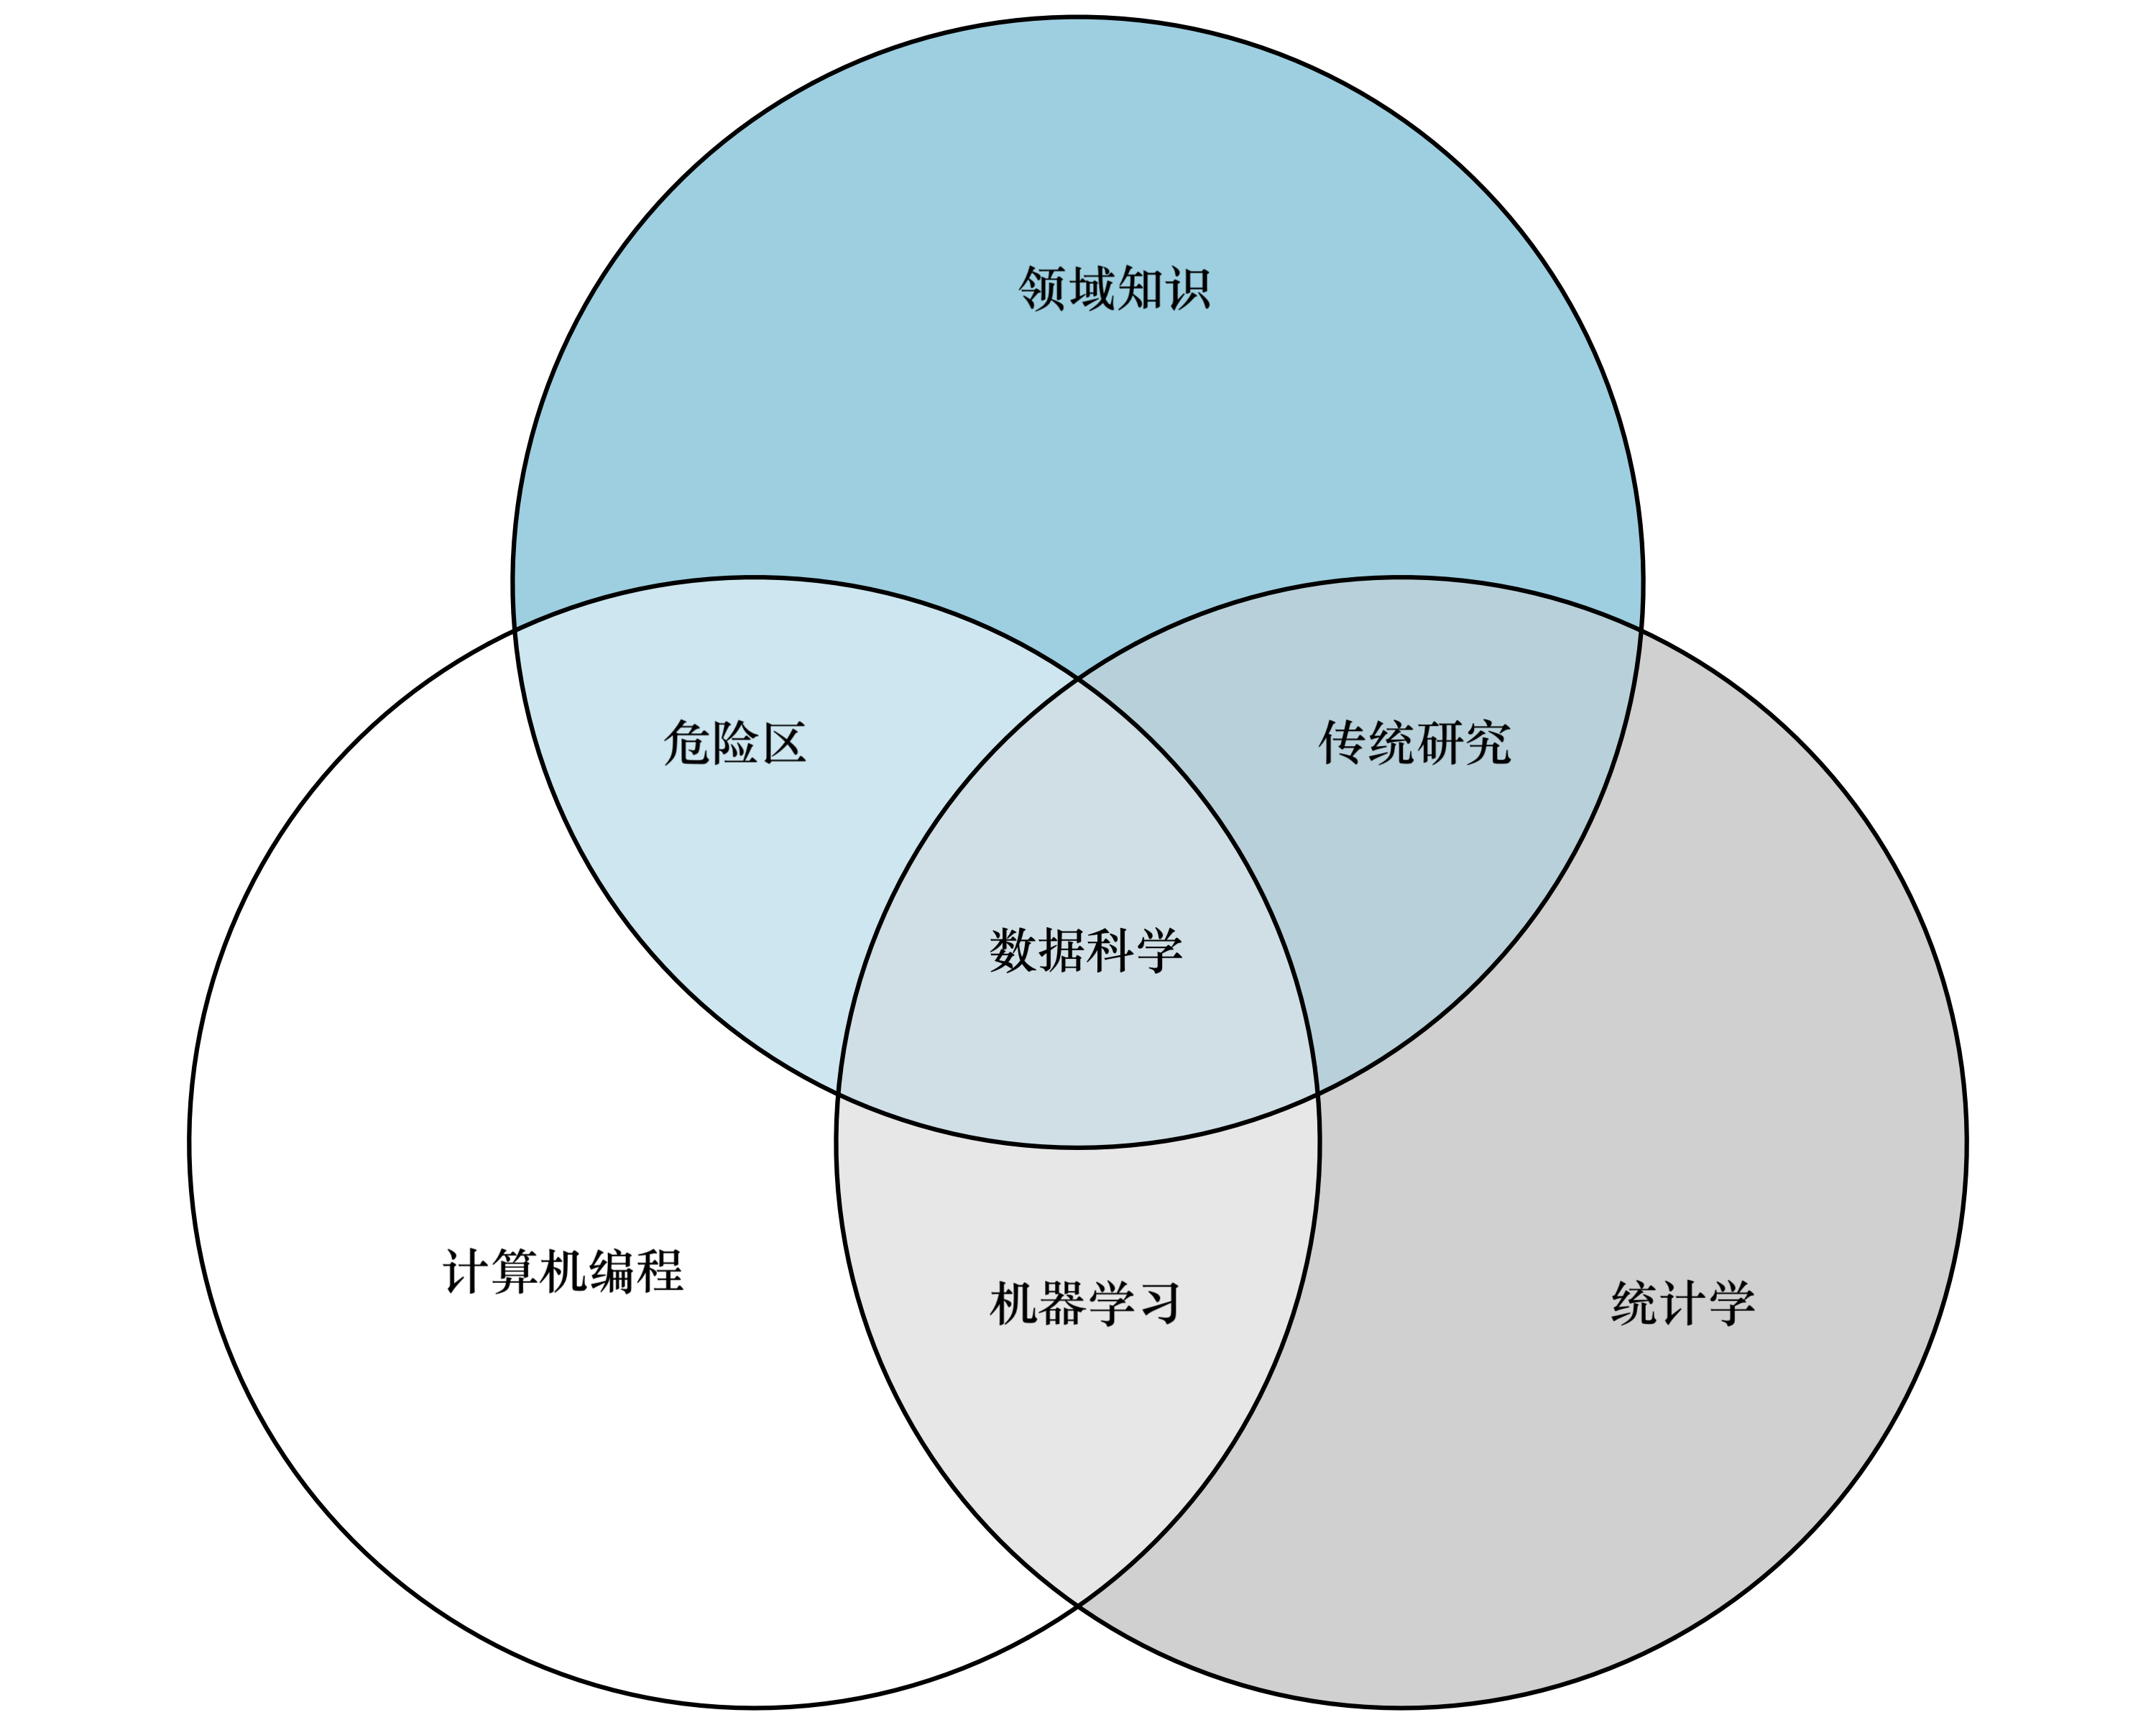
\includegraphics{images/figure1_1.png}
\caption{图1.1数据科学的能力结构(Ozdemir, 2016)}
\end{figure}

\hypertarget{ux6570ux636eux79d1ux5b66ux4e0eux8bedux8a00ux7814ux7a76}{%
\section{数据科学与语言研究}\label{ux6570ux636eux79d1ux5b66ux4e0eux8bedux8a00ux7814ux7a76}}

数据科学与语言研究之间存在紧密的关系,数据科学方法和技术已经在语言研究领域中发挥了重要作用。

\begin{enumerate}
\def\labelenumi{\arabic{enumi}.}
\item
  \textbf{语言数据的收集和处理:} 数据科学提供了丰富的工具和技术,用于收集、存储、管理和处理大规模的语言数据。这包括文本、语音、图像和视频数据。语言学家可以利用这些数据来研究语言的不同方面,如语法、语义、语音学和语用学。
\item
  \textbf{自然语言处理(NLP):} 自然语言处理是数据科学中的一个重要分支,专注于使计算机能够理解和生成人类语言。NLP技术被用于机器翻译、文本分类、情感分析、命名实体识别等各种语言相关任务,这些任务对于语言研究也具有重要意义。
\item
  \textbf{文本挖掘和信息检索:} 数据科学方法可以帮助研究人员从大规模文本数据中提取有关特定主题、情感、趋势或模式的信息。这对于语言研究者来说是宝贵的,因为他们可以更轻松地分析和理解大量的文本数据。
\item
  \textbf{语言模型和机器学习:} 机器学习方法在语言研究中得到广泛应用,尤其是在构建语言模型和自动语言处理工具方面。深度学习模型如循环神经网络(RNN)和变换器(Transformer)已经取得了在自然语言处理任务中的重大突破,如机器翻译和文本生成。
\item
  \textbf{社交媒体分析:} 数据科学方法使研究人员能够分析社交媒体上的大规模语言数据,以了解公众的观点、情感和趋势。这对于社会语言学和舆论研究非常重要。
\item
  \textbf{语言多样性研究:} 语言研究可以通过分析不同语言和方言的数据来深入了解语言多样性。数据科学方法可以帮助研究人员跟踪语言变化、保护濒危语言以及研究全球范围内的语言多样性。
\item
  \textbf{语言习得研究:} 数据科学方法可以用来分析语言习得过程中的大量语言数据,从而帮助我们更好地理解儿童和成人如何学习语言。这有助于改进语言教育和幼儿教育方法。
\item
  \textbf{语言变化和历史研究:} 数据科学可以用来分析历史文本和语料库,以研究语言的演变和变化。这对于历史语言学家和语言历史学家来说是一个有趣的领域。
\item
  \textbf{跨文化和跨语言研究:} 数据科学可以帮助研究人员进行跨文化和跨语言的比较研究,以了解不同语言和文化之间的共同点和差异。
\item
  \textbf{情感分析和情感研究:} 情感分析是数据科学中的一个重要领域,它涉及分析文本和语音数据中的情感和情感状态。这对于了解情感表达和情感健康在语言中的作用非常有用。
\item
  \textbf{语言治疗和康复:} 数据科学方法可以用于开发语言治疗工具和康复应用程序,以帮助言语和语言障碍患者改善他们的交流能力。
\end{enumerate}

语言研究数据几乎包含了数据的各种类型,既有结构性数据也有非结构性数据。这对于语言研究者的数据处理能力提出了很高的要求。数据科学家大体上包含了三个能力模块:数学/统计学,专业知识,计算机编程。

语言研究者在数据处理方面的优势,最主要的体现在对于研究领域的知识背景熟悉。这对于数据预处理中的一些决策,如判断缺失值,偏异值以及采取相应的措施是十分重要的。此外,对于研究领域的背景知识的了解,对于探索性数据分析和数据可视化的思路上有很大的帮助。如果将语言研究中的数据处理任务外包给统计学或者计算机科学背景的专业人士,他们缺乏对于研究领域的知识,会阻碍数据的处理,探索性分析和建模。因此,新时代的语言研究者具备一定的数据科学知识与技能是十分重要的。

数学和统计学的能力是语言研究者,特别是文科背景的语言研究者担忧的方面。然而,数据科学是一个应用性科学,不同类型的数据处理对于统计能力的要求不同,并不一定都要求十分深厚的数学背景。比如,文本处理和一些语料库的基本数据统计,要求理解描述性统计的基本知识,结合不同的公式,理解其中区别就可以了。再例如一些推断性统计检验,需要理解一些基本的数据分布和概率假设。这些内容理解上并不难,具体的计算则可以通过计算机完成,并不需要非常强的人工计算能力。
第三个能力模块是电脑编程。所谓电脑编程就是用编程语言将自己需要做的事转化为指令传递给计算机。大部分文科背景的研究者都有学习外语的经历,电脑编程与之类似,需要学习编程语言的函数(相当于词汇)和语法格式。和学习自然语言一样,这是一个过程,并且其中会伴随一些困难,但这些都是暂时的,笔者认为在未来的十年里,在量化模式的语言研究中,通过编程的方式处理语言和语言应用中所产生的数据是大势所趋。

综上所述,数据科学在语言研究中扮演了多重角色,从语言数据的处理和分析到应用产品的开发,都对语言研究领域产生了积极的影响。这个交叉领域将继续蓬勃发展,为我们更好地理解语言和改进语言相关应用提供更多机会。

\hypertarget{ux7b2cux4e8cux7ae0-rux8bedux8a00ux4e0eux6570ux636eux79d1ux5b66}{%
\chapter{第二章 R语言与数据科学}\label{ux7b2cux4e8cux7ae0-rux8bedux8a00ux4e0eux6570ux636eux79d1ux5b66}}

\hypertarget{rux8bedux8a00ux7b80ux4ecb}{%
\section{R语言简介}\label{rux8bedux8a00ux7b80ux4ecb}}

R语言的历史可以追溯到20世纪90年代。R语言最初是由奥克兰大学的罗斯·伊哈卡(Ross Ihaka)和滑铁卢大学的罗斯·伊哈卡(Robert Gentleman)和纽约大学的共同开发的。他们二人的名字都以R开头所以将其发明的语言成为R语言。起初是为了解决自己在统计学研究中遇到的问题而创建了R语言。(Ihaka, R. (2011). The R Project: A brief history and thoughts about the future. Presentation given at the University of Otago.)

R语言最早的版本基于S语言句法实现。R语言从S语言继承了很多特性,但也进行了许多改进和扩展,使其变得更加强大和灵活。

R语言为统计学家和数据分析师提供一个强大的计算和可视化工具。它提供了丰富的统计分析函数和图形绘制函数,使用户可以在一个集成的环境中进行数据的处理和分析。R语言是一个跨平台的编程语言,可以在不同操作系统上运行,如Windows、Mac和Linux。

R语言在统计学界和数据科学领域得到了广泛的应用和认可,并且在金融、医药、社会科学等领域中都有大量使用者。同时,随着人工智能和机器学习的发展,R语言在机器学习和人工智能等领域也有着广泛的应用。

由于R语言的开源特性,R语言的社区也非常活跃,有很多开源的扩展包和工具可以使用,用户还可以贡献自己的包或作为志愿者参与R语言项目的发展。

值得一提的是,R语言的学习门槛并不高。它的语法简洁易懂,对于初学者来说也比较友好。因此,R语言在大学和研究机构的教学中得到了广泛应用。它拥有丰富的学习资源和社区支持(例如,R语言在线手册:\url{https://cran.r-project.org/manuals.html}; R语言图书:\url{https://www.r-project.org/doc/bib/R-books.html} )。即使是没有编程经验的初学者也能够快速上手。通过学习R语言,人们可以更好地理解和应用数据,从而为决策提供更多的支持和建议。因此,无论你是研究者、数据分析师还是爱好者,学习和掌握R语言都是一个值得投入的宝贵的时间和精力。

\hypertarget{r-studioux7b80ux4ecb}{%
\section{R-Studio简介}\label{r-studioux7b80ux4ecb}}

R语言可以在计算机上通过终端命令直接运行,也有自己的图形界面。但是RStudio 是最适用于初学者的R 编程的集成开发环境(integrated development environment,IDE)。使用者可以从 \url{http://www.rstudio.com/download} 下载并安装。其中免费版已经可以满足数据科学的需求了。

它提供了许多功能,如代码编辑器、调试器、数据可视化和包管理器等,使得R语言的学习和使用变得更加方便和高效。R-Studio被广泛用于数据科学、统计分析、机器学习和数据可视化等领域。

\begin{figure}
\centering
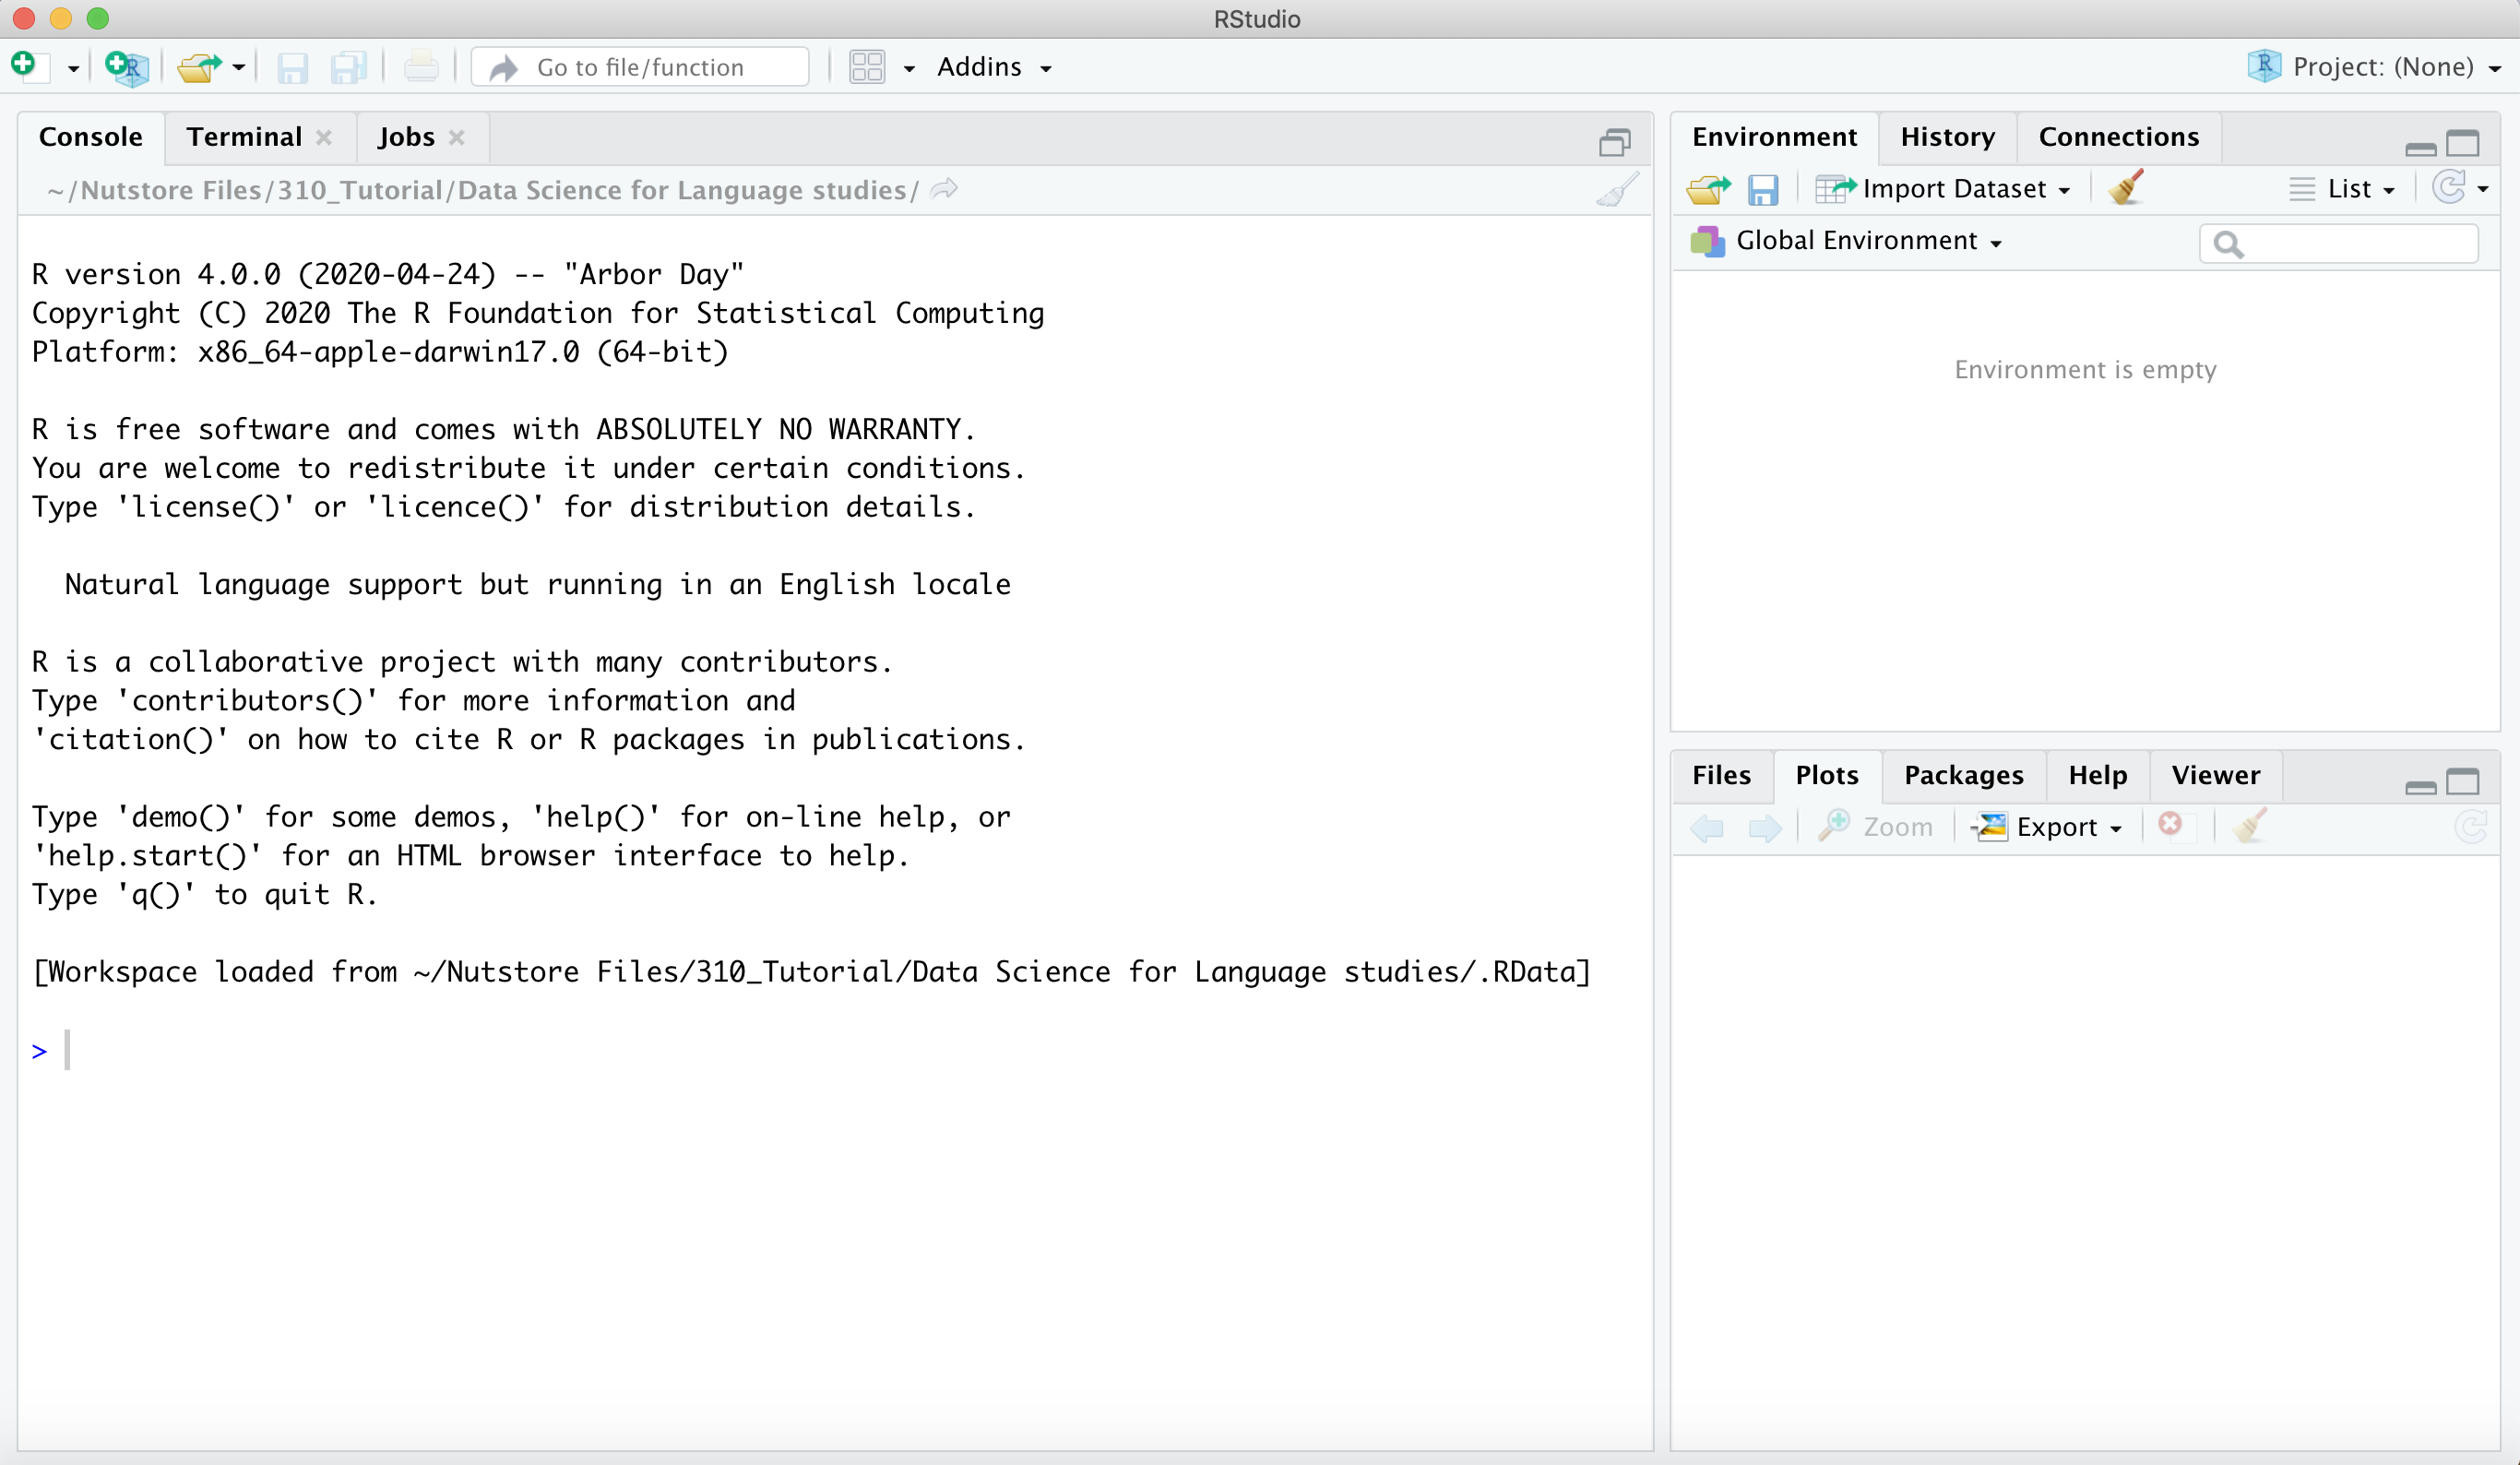
\includegraphics{images/2.1.png}
\caption{图2.1 R-studio初始化}
\end{figure}

首先,初始界面有3个区域。在图中左侧区域是输入和运行代码区域,右侧上部的区域目前选中的是environment也就是环境变量的显示窗口。当前并没有输入任何代码,所以环境变量的窗口是空白。在右侧下部,对窗口有5个不同的按键:文件(File),制图(Plots),程序包(Packages),帮助(Help),视图(Viewer)。目前选中的是作图窗口。
在代码运行窗口,我们可以输入命令,然后按回车键即可运行命令。如果我们想要将命令写成脚本,方便重复使用,修改,那需要新建一个脚本文件。

我们推荐两种方式书写脚本,一种是把脚本文件格式,另外一种是Rmarkdown文件格式。
脚本文件格式

\begin{figure}
\centering
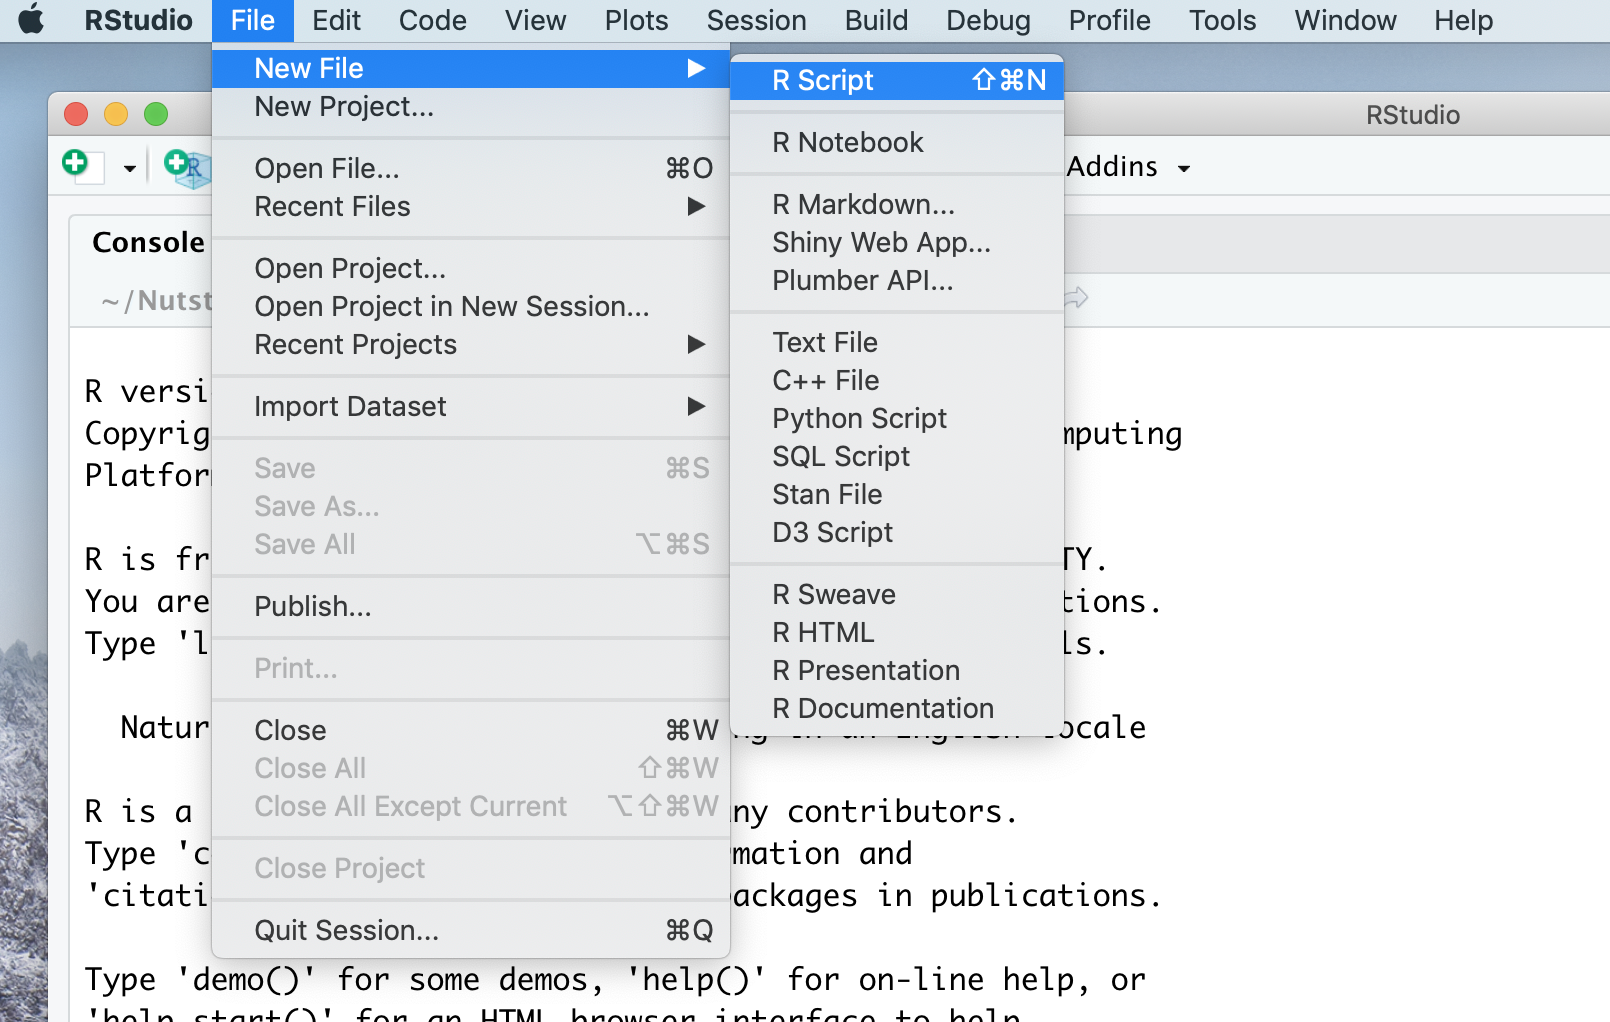
\includegraphics{images/2.2.png}
\caption{图2.2 新建脚本}
\end{figure}

当我们新建了一个脚本文件,就会出现一个窗口。原先的代码运行窗口,变换到了左边的下部,而在左边上部出现了一个新的窗口。这就是脚本书写窗口。在这里书写的脚本,我们可以通过选中来运行。
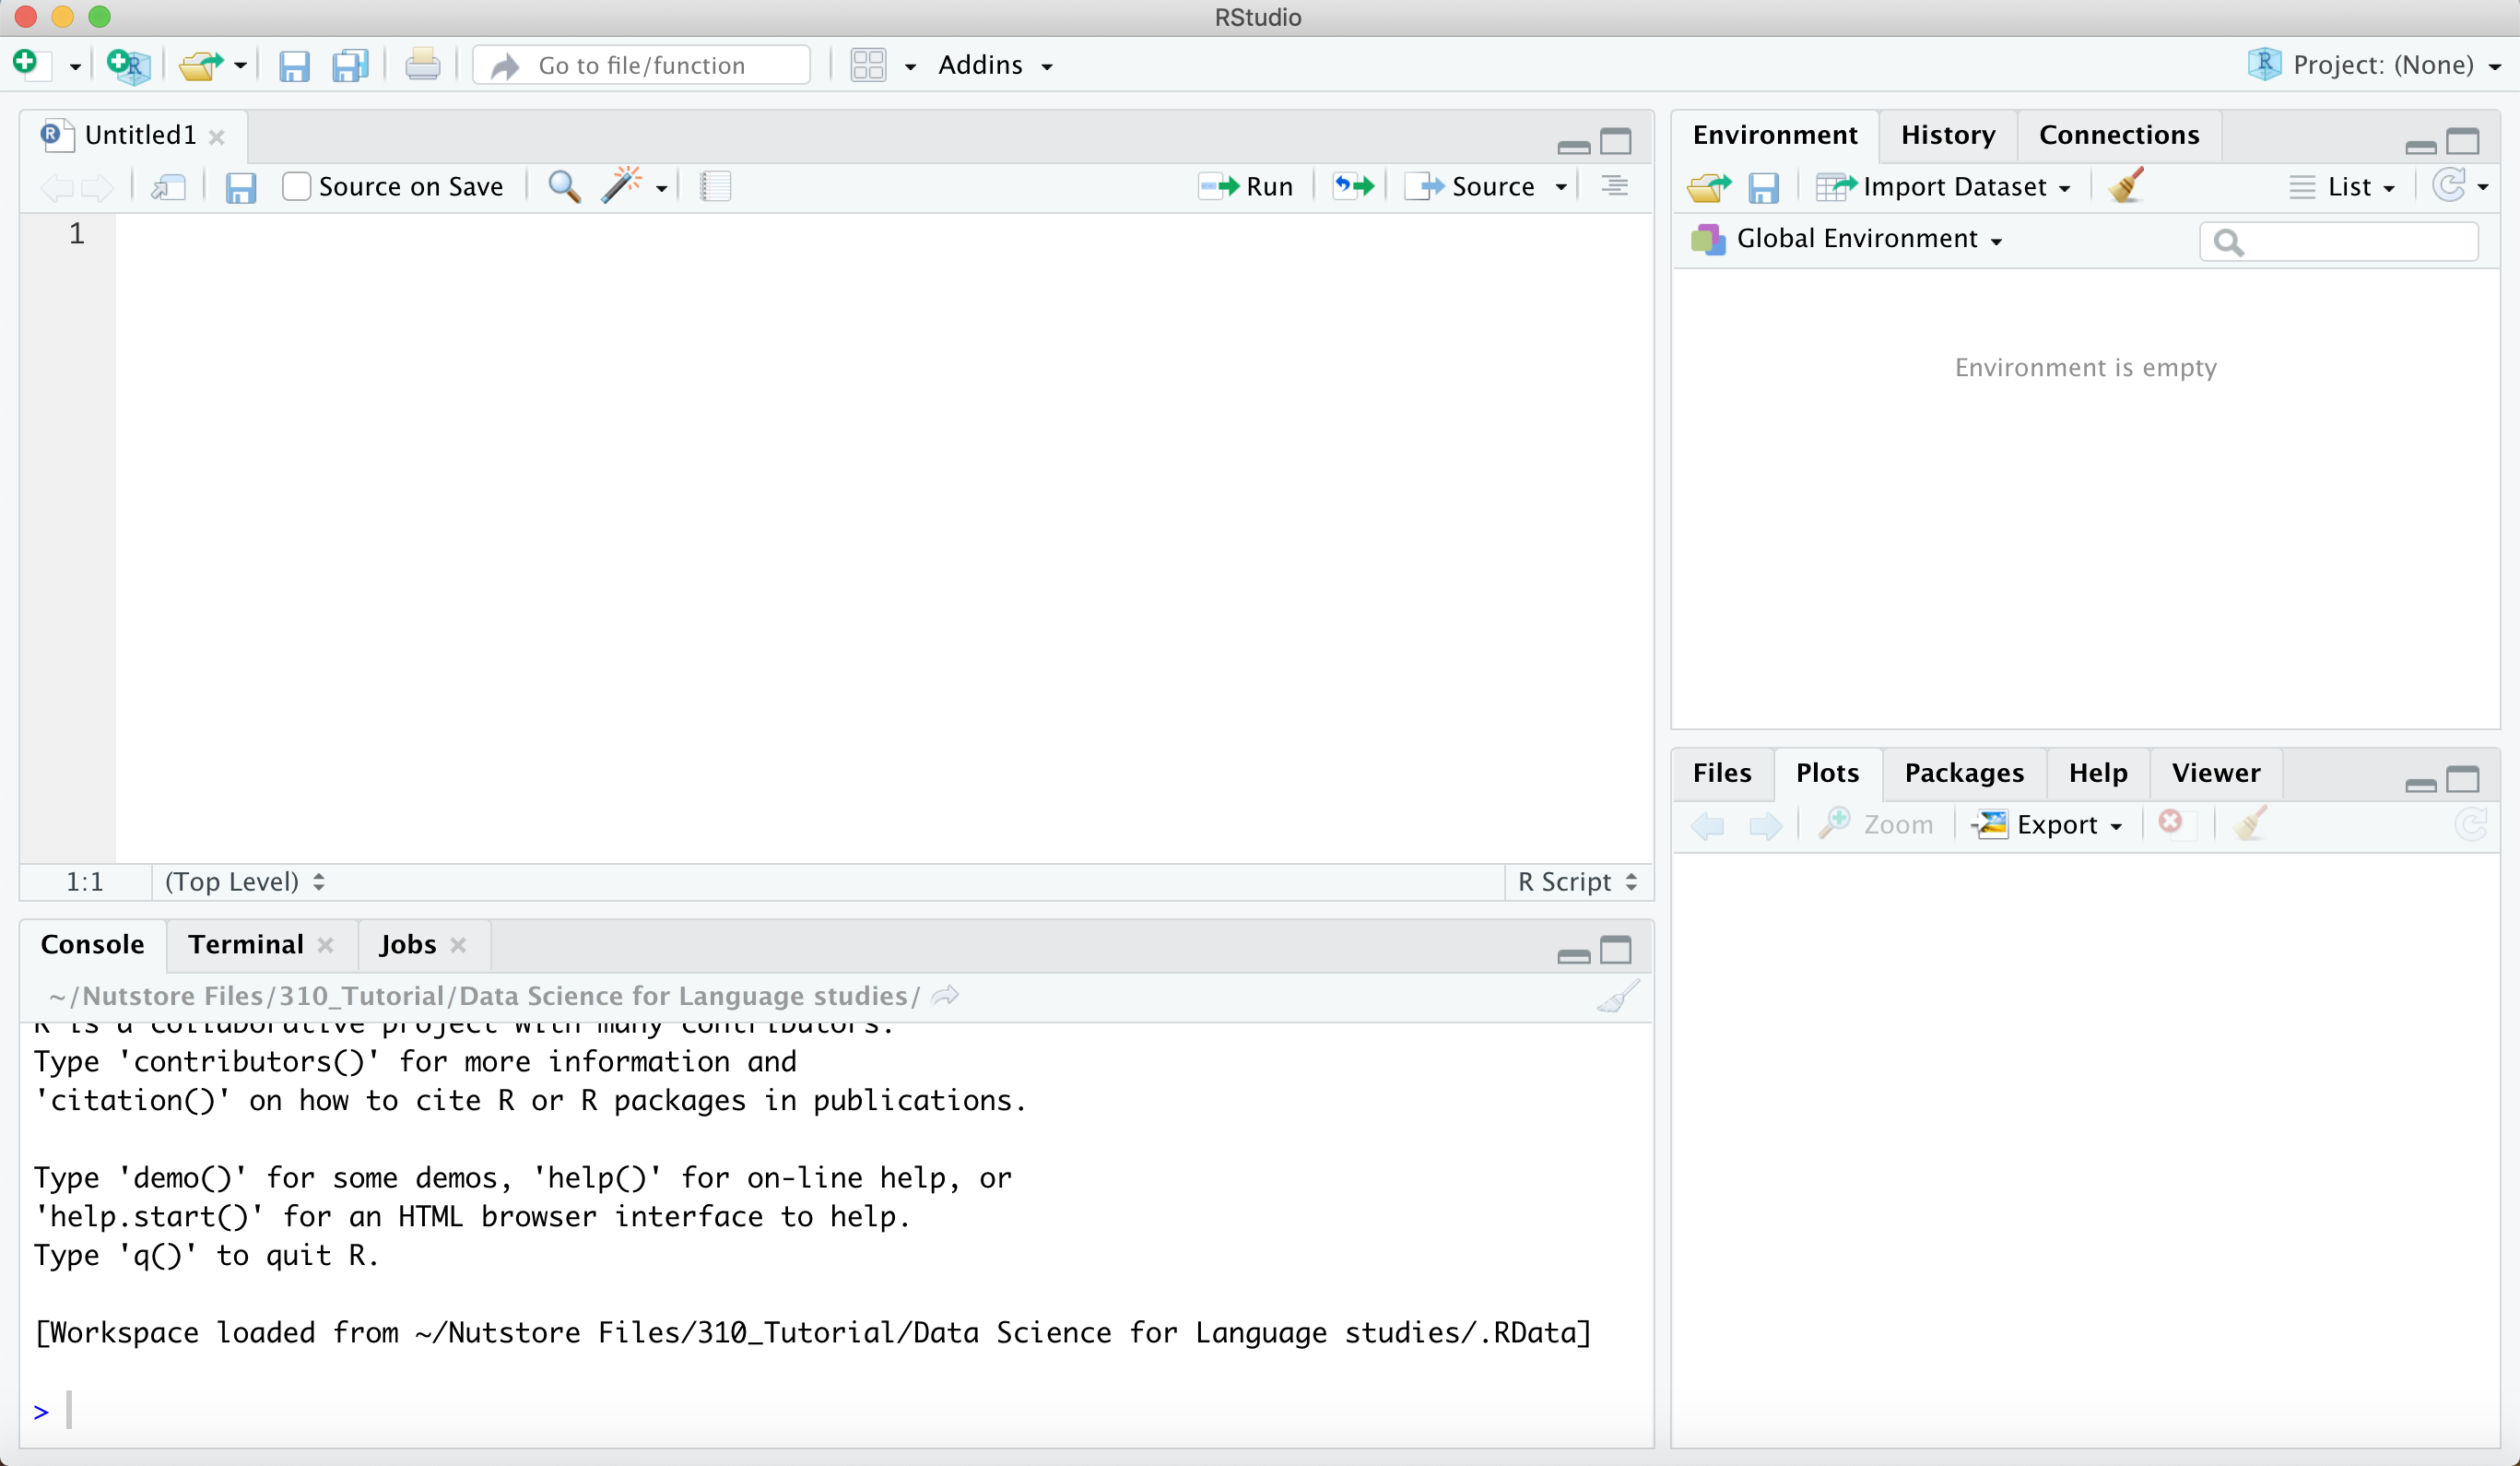
\includegraphics{images/2.3.png}

R-Markdown文件

r-markdown是一种可复制性更好的数据分析记录报告文件格式,符合可读性统计编程(literate statistical programming)的理念。它可以将数据分析的代码,统计建模的细节和解释说明的文字以及可视化的图片统一集成在一个文件当中。这个文件可以输出网页格式、PDF或者文档。
可读性统计编程(literate statistical programming)是基于可读性编程(Literate programming)创造的新的一个概念。可读性统计编程将统计分析过程的代码和相关描述融合在一个文件当中。这样读者既可以了解到分析过程,同时也可以通过作者的数据,运行代码得到相同的结果。这样最大程度的保证研究数据分析的可再生性(reproducibility)。
从学科发展的角度,研究可再生性可以提高研究的科学性。一个研究能否成为人类知识的一个部分,取决于他人是否能够复制验证这个研究的结论。当然,不同学科的可复制性本身有差异。比如,复制一个化学实验比复制一个心理学实验要容易的多,因为化学实验的对象是物质,物质本身的特性是稳定,化学反应的条件是可控的。而心理学实验的对象是人的心理,人本身是存在变异性的,心理活动产生的条件控制难度远远大于化学实验。但是,对于一项心理学研究而言,至少可以实现同行使用此项研究的数据,按照研究者的方法可以得到相同的结论,即可再生性。可复制性最低的门槛就是可再生性。
其次,提高研究的可再生性,公开研究分析过程和代码,可以减少重复研究的浪费。研究者可以利用别人现有的研究过程和代码,在此基础上进一步进行研究。而不需要从头开发。此外,研究的过程不是线性的,一蹴而就的。合作者、期刊编辑、外审专家都会对研究数据处理过程提出一些意见。难免要进行反复修改,模型调试,数据增减,需要不断重复某些数据分析过程。通过编程高效重复数据处理过程,会使研究者将精力放在研究问题上,而不是重复机械劳动上。同时也保证研究结果准确。
对于个人来说,研究者如果有很强的可读性统计编程和可再生性意识,并且准备在研究中实践。这种观念本身就会影响研究数据的管理和组织。使得研究工作更为高效。其次,研究者通常会长期从事某一领域的研究,其研究具有一定的继承性。通过可读性统计编程和脚本管理,研究者可以轻松利用自己过去某个研究的分析过程,实现复利迭代。
对于研究团队而言,可再生研究可以提高团队协作的效率。如果数据分析过程非常透明易懂,那么合作者更加容易融入团队,分工协作。
可再生的研究通常能够让别人更加相信。同行会使用你的数据分析中某些步骤或者代码,并且引用你的论文可以增加你的研究影响力。

首先,点击新建文件,然后选择R-markdown。
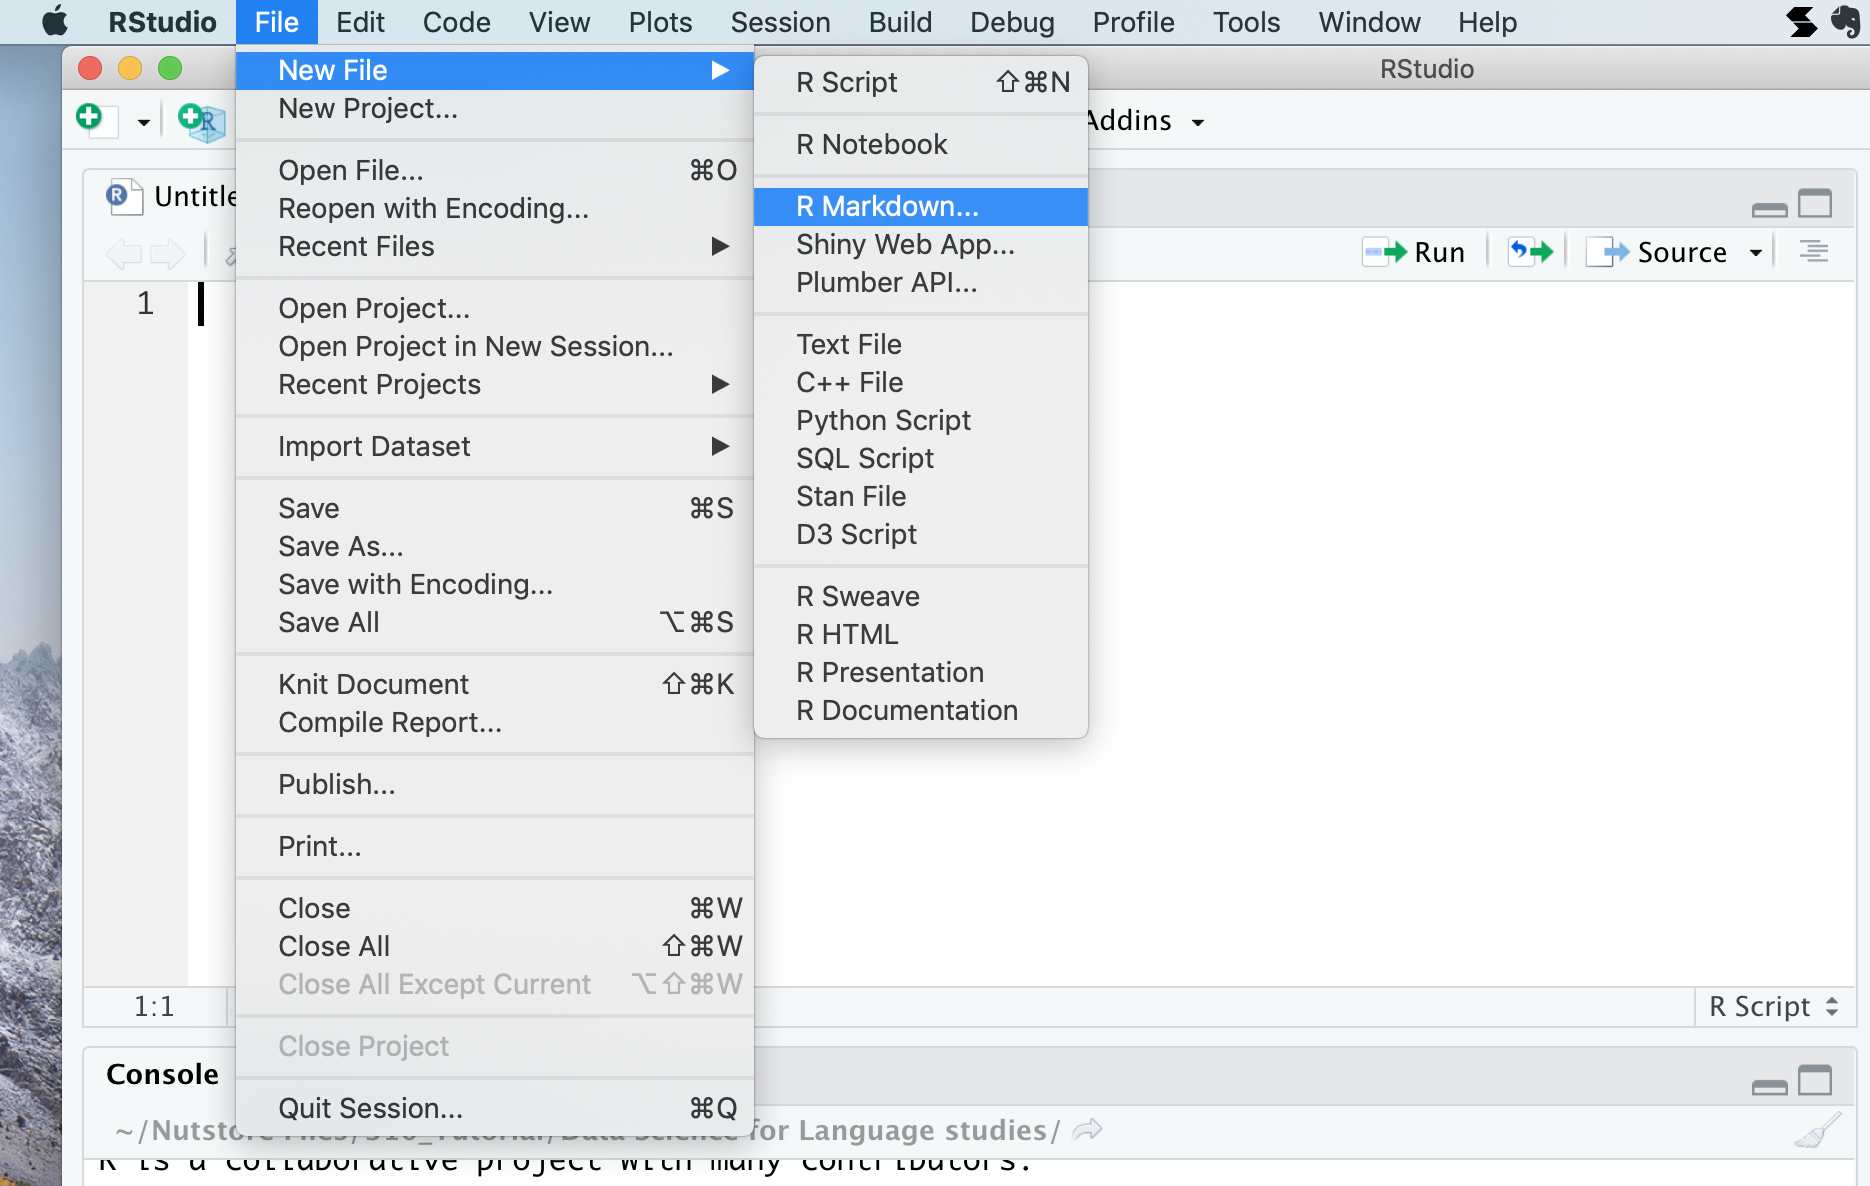
\includegraphics{images/2.4.png}

在弹出的对话框中,你需要选择文件输出的类型,比如这里我们选择网页格式。同时你可以填写相应的文件标题和文件作者名称。完成以后点击OK就可以了。
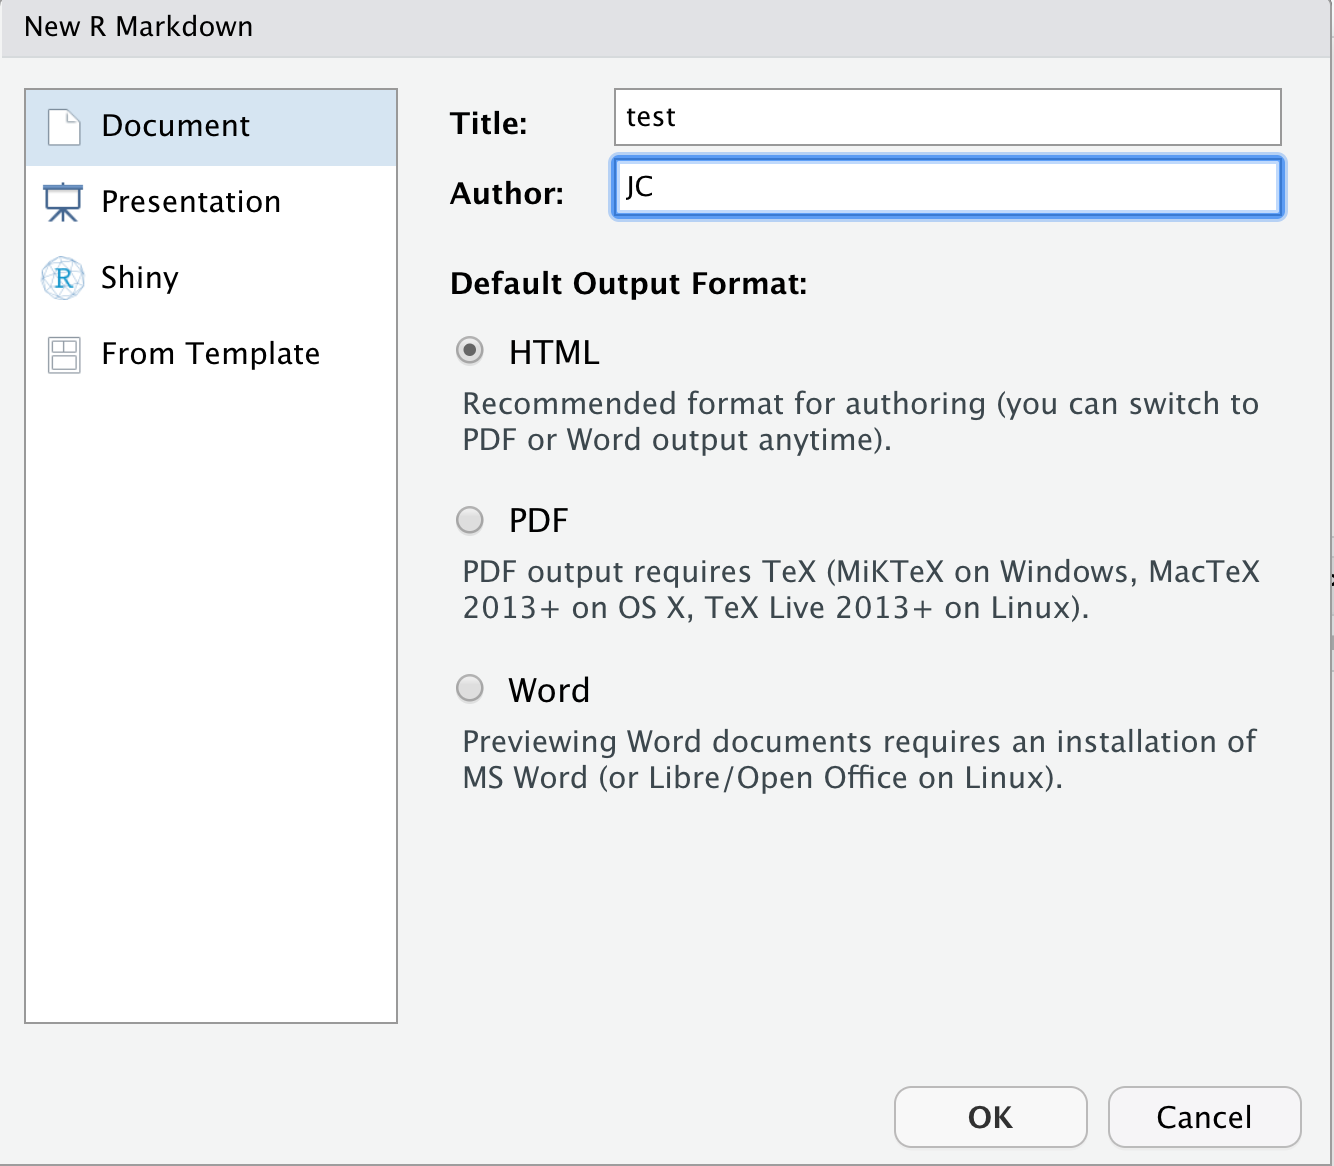
\includegraphics{images/2.5.png}

\begin{figure}
\centering
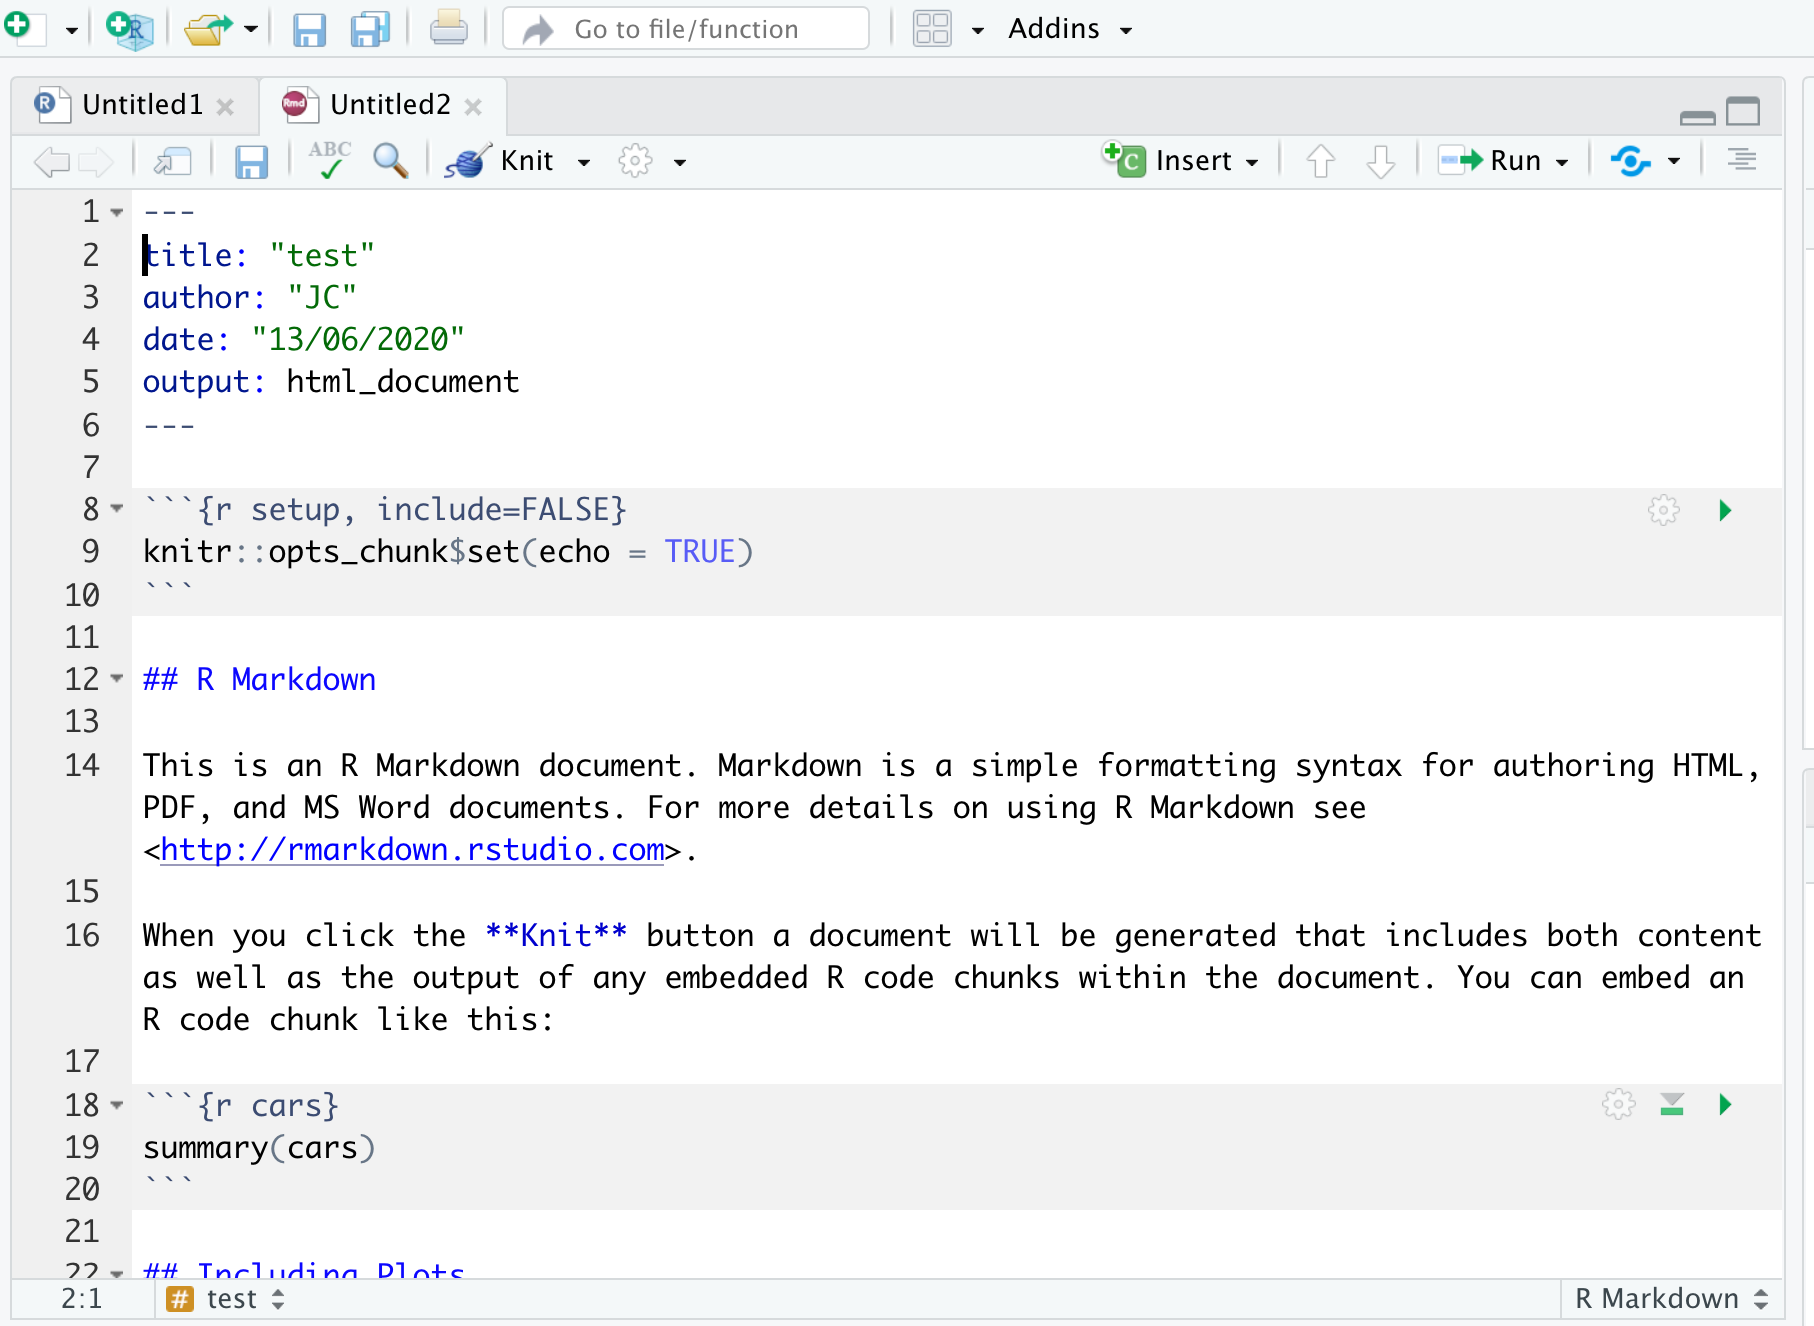
\includegraphics{images/2.6.png}
\caption{图2.6 R-Markdown初始参数设置}
\end{figure}

编辑完成以后,需要将R-markdown文件先命名并且保存。然后,我们可以点击文件上面有一个knit按钮(配有一个织毛衣图示),R-studio就会将文件转换成之前设置的格式。
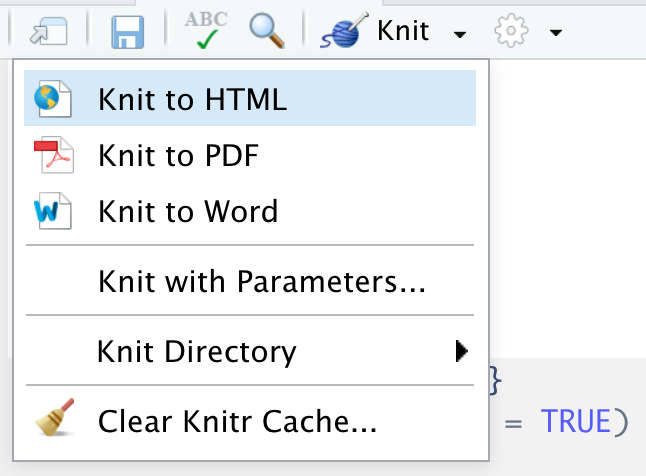
\includegraphics{images/2.7.png}

这里我们将文件输出为网页格式。

\begin{figure}
\centering
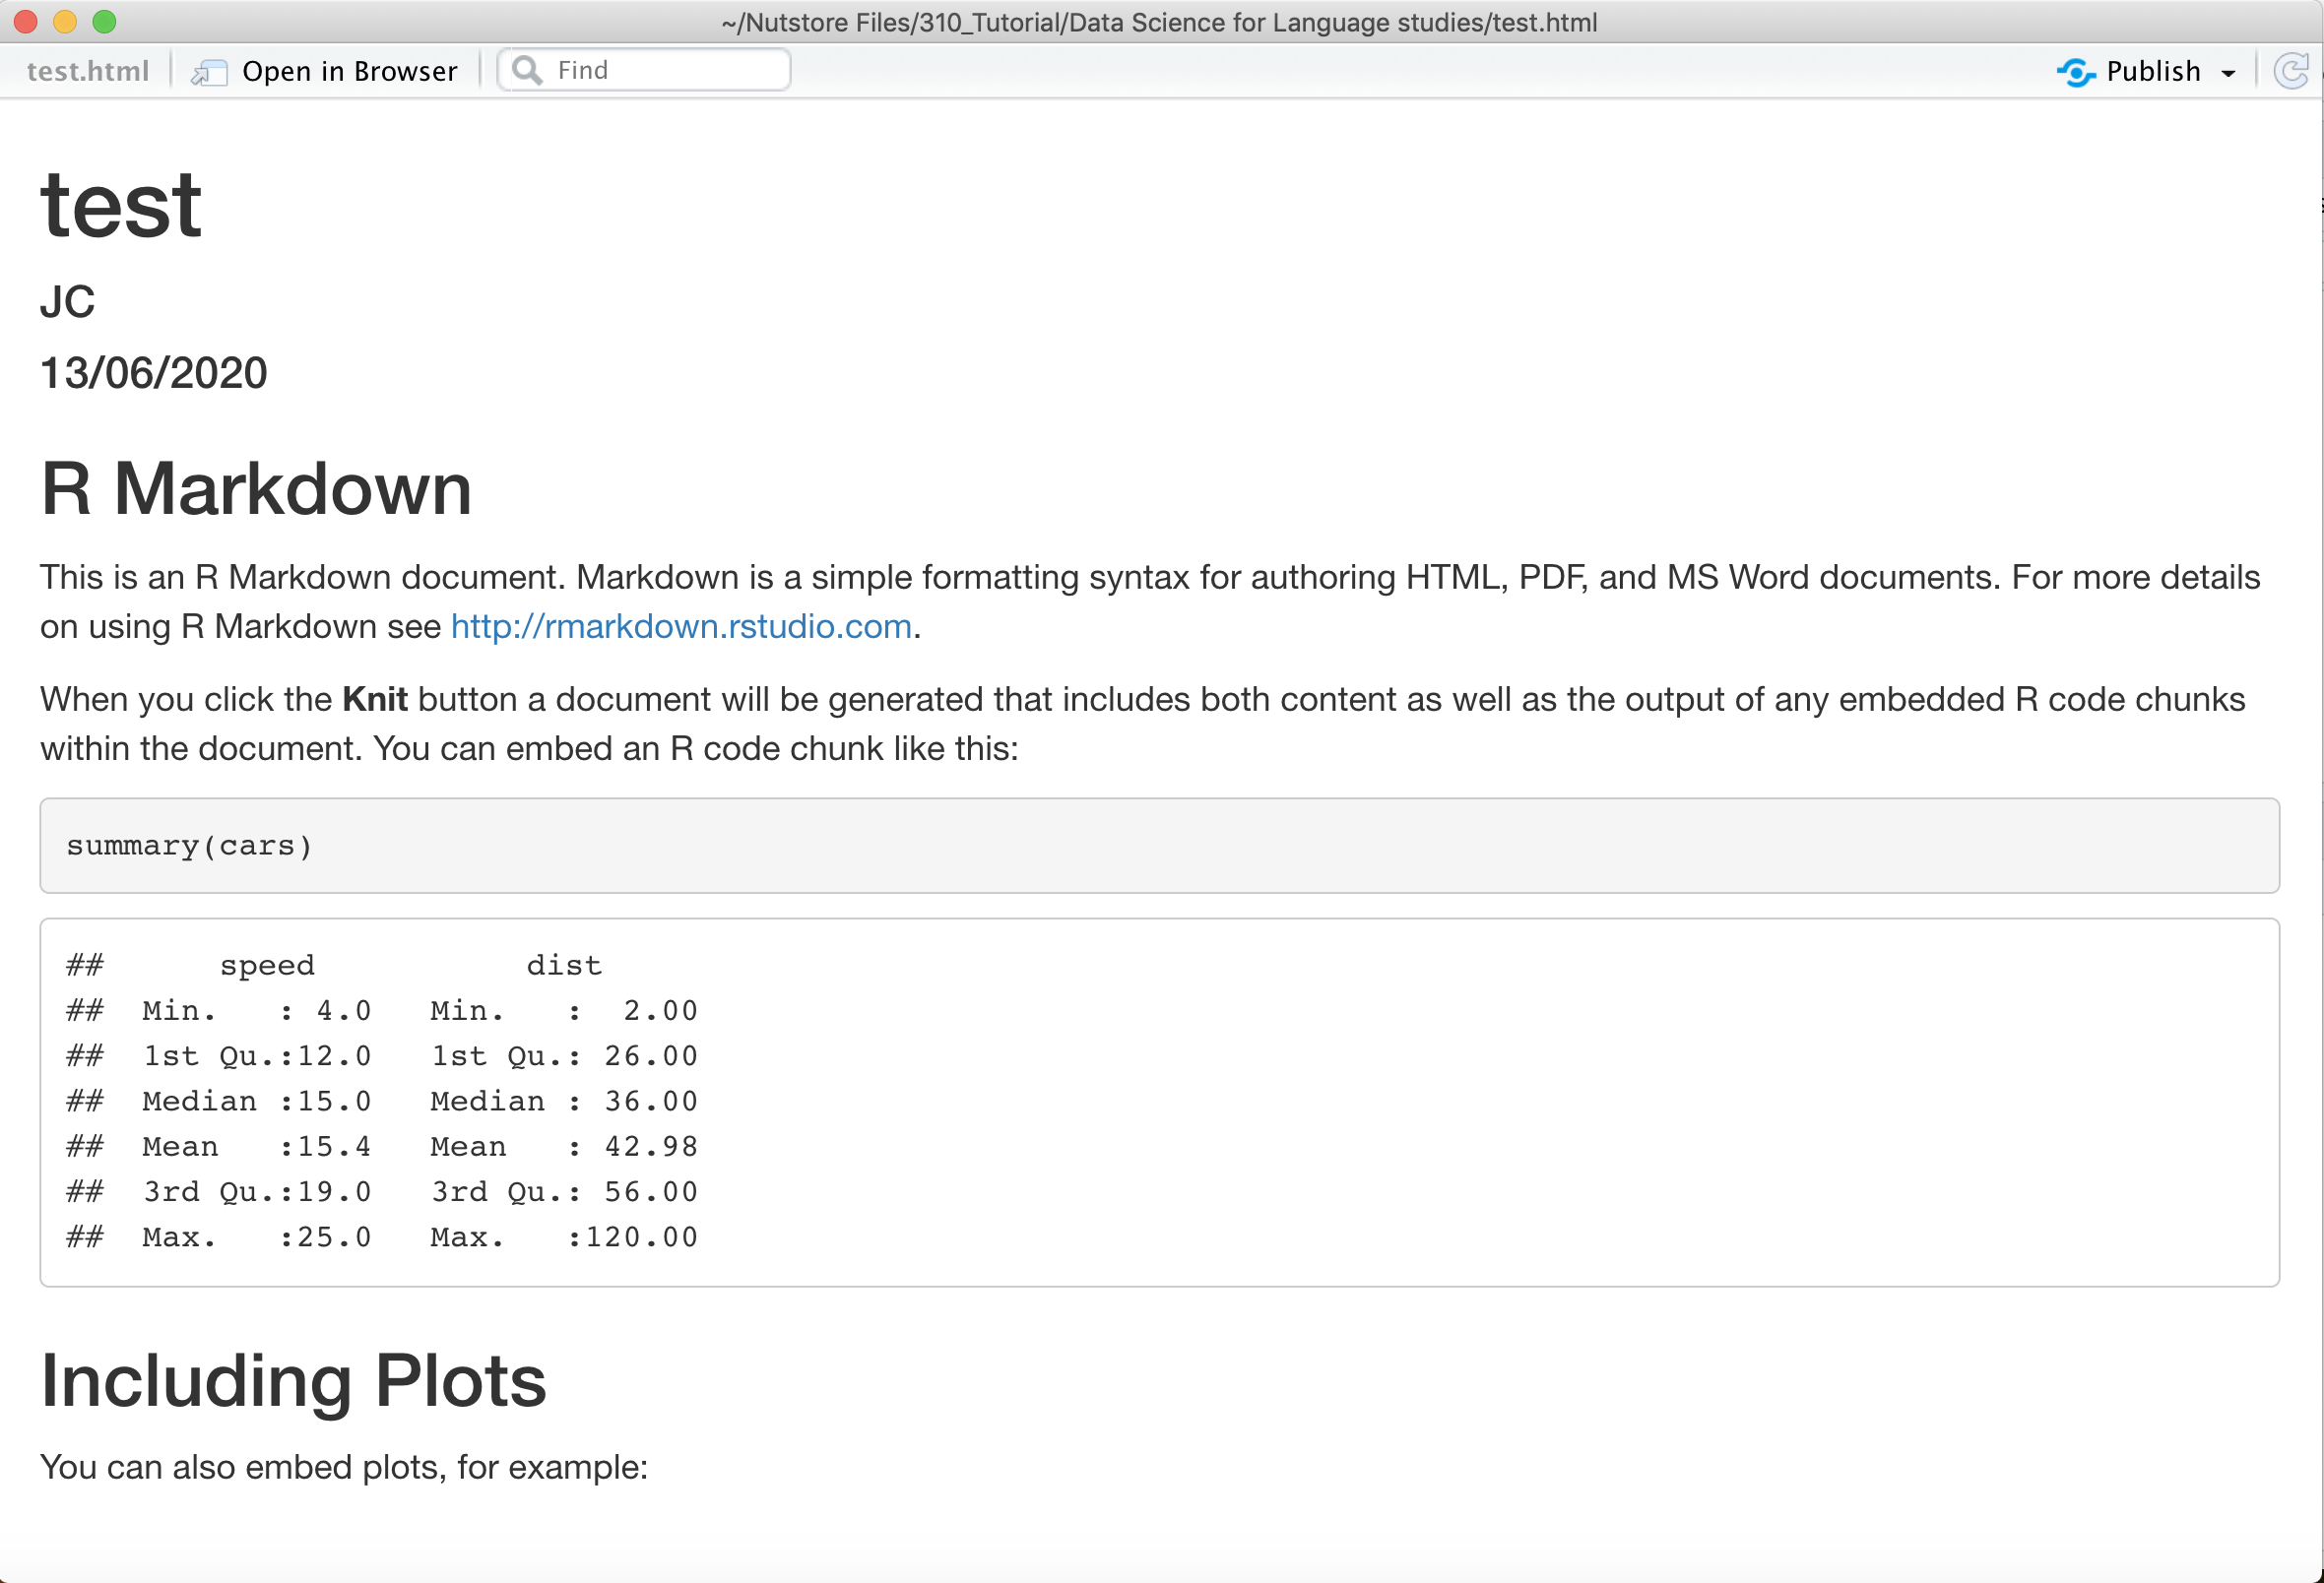
\includegraphics{images/2.8.png}
\caption{图2.8 网页文件示意图}
\end{figure}

建立R-project
在数据处理中,我们通常会将输入和输出的数据放在一个文件夹里,每次导入数据的时候,我们需要输入绝对或者相对的路径。但是当你的合作者在另外一台电脑上打开你的文件夹时,这个绝对或者相对的路径就会发生错乱。因此,为了保持编程环境的相对稳定,我们可以为自己的数据处理项目建立一个project文件夹。当我们有一个project文件夹以后,R-studio里面就只需要输入相对路径。特别值得注意的是,无论是在云端同步,还是通过移动硬盘U盘等复制,这个文件夹是一个独立的编程环境。

首先我们点击文件新建项目。
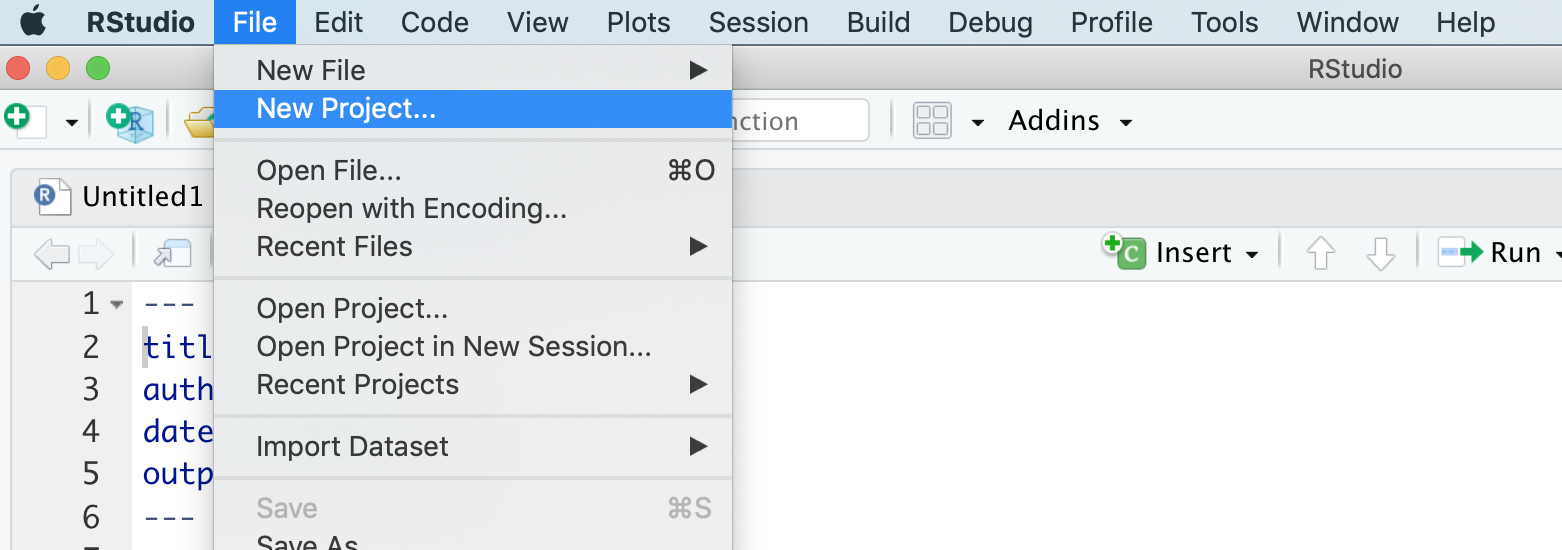
\includegraphics{images/2.9.png}
然后我们可以选择新建项目或者使用已有的文件夹。
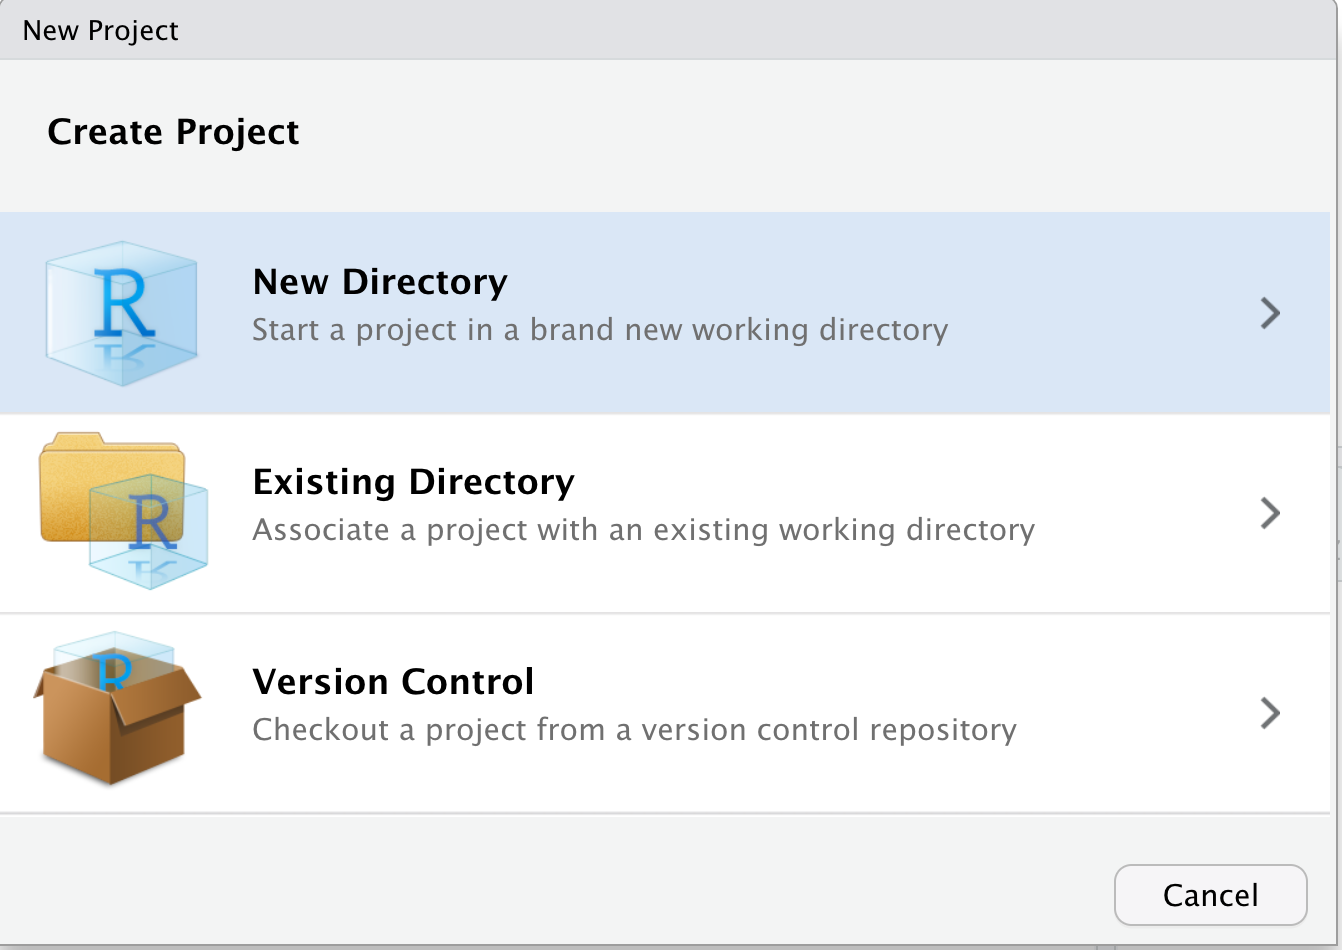
\includegraphics{images/2.10.png}
如果选择新建项目,那么需要给项目文件夹一个名称,并设置文件夹的位置。
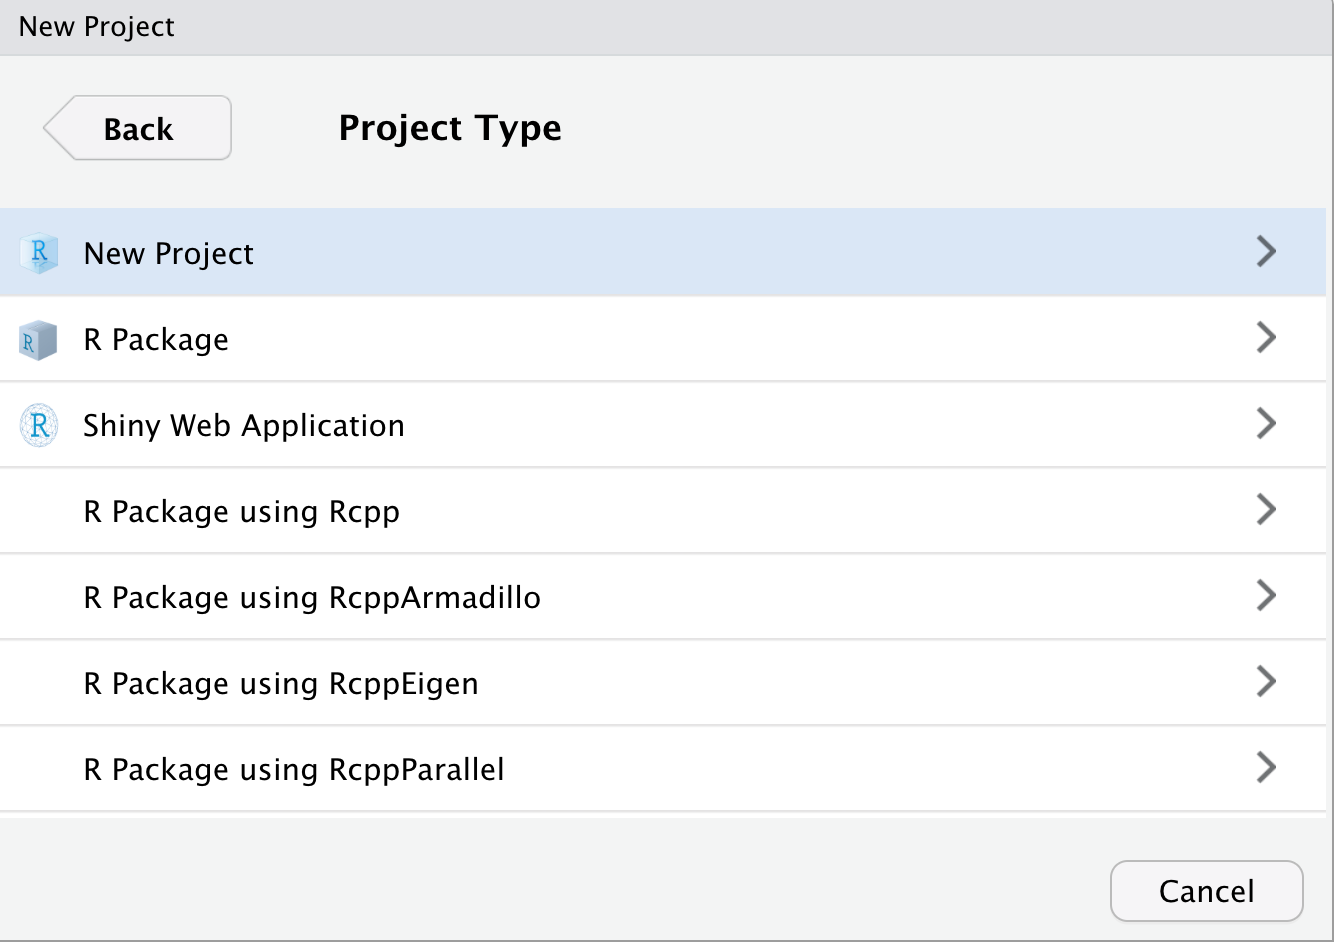
\includegraphics{images/2.11.png}
新建项目以后,在所指定的路径,就会发现一个新的文件夹。
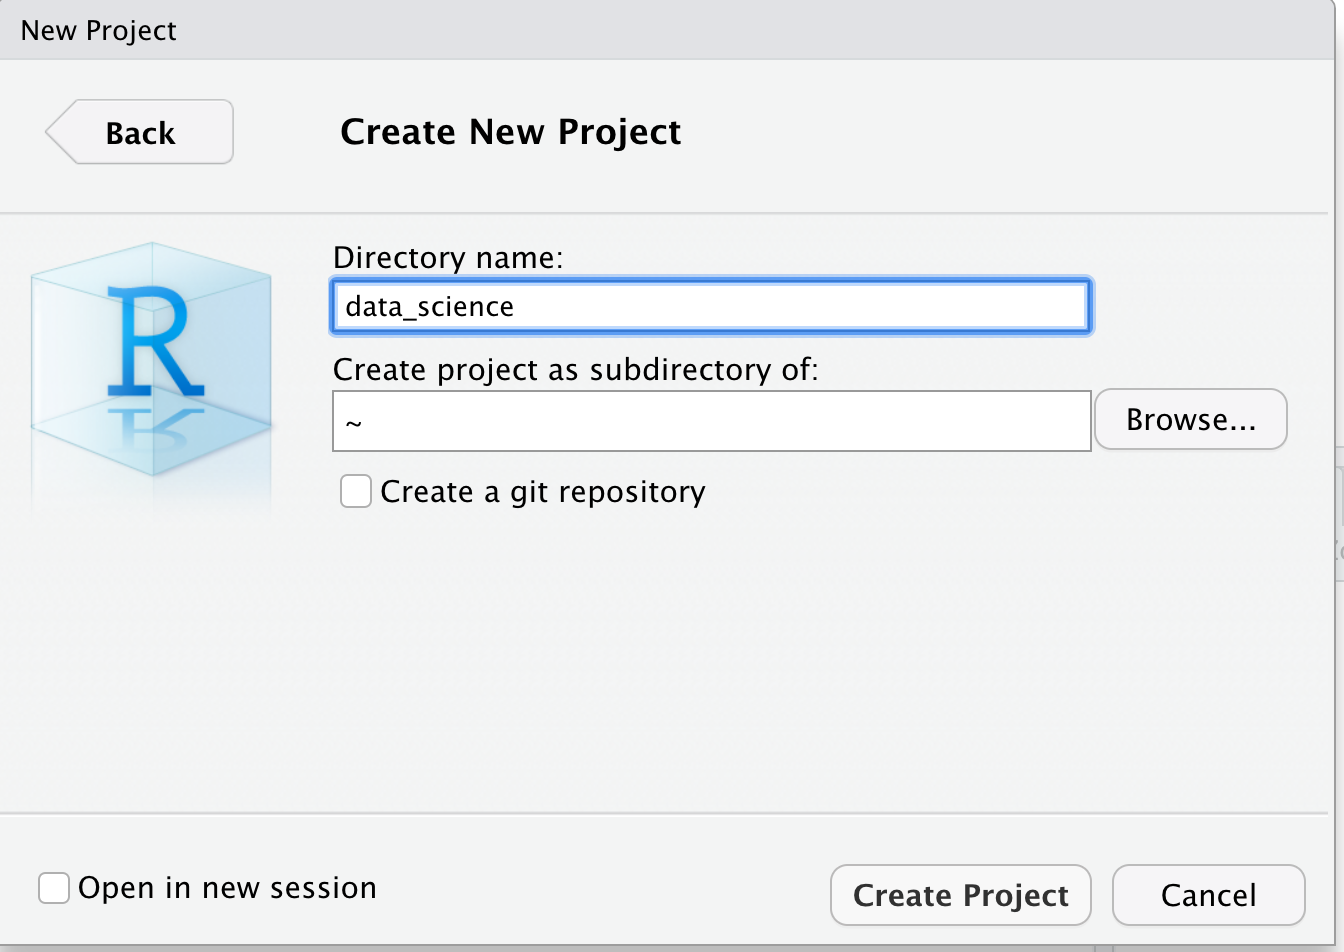
\includegraphics{images/2.12.png}
在该文件夹内部,会有一个R-project文件。以后每次开始项目时,双击这个文件就会自动打开一个项目编程环境,里面所有路径都可以是相对路径。

R-Studio支持多种操作系统,包括Windows、Mac和Linux。它具有快速和高效的数据处理能力,可以处理大型数据集并提供交互式可视化。此外,R-Studio还允许用户通过插件和扩展来自定义其功能,以满足不同的需求。R-Studio还提供了一些方便的功能,如代码自动补全和语法高亮等,使得编程变得更加轻松和流畅。通过R-Studio,用户可以快速编写和测试代码,并进行数据可视化和统计分析。
此外,R-Studio还提供了丰富的教程和文档,可以帮助用户快速上手并解决问题。它还有一个活跃的社区,用户可以在这里交流经验和技巧,获取支持和建议。

总之,R-Studio是一款功能强大、易于使用、高度可定制、跨平台的数据科学工具,可以帮助用户轻松地掌握R语言并进行高效的数据处理和分析,为用户提供了全面的数据分析解决方案。无论是进行统计分析、数据可视化还是机器学习,R-Studio都能够帮助用户实现他们的目标。

\hypertarget{r-packageux7b80ux4ecb}{%
\section{R package简介}\label{r-packageux7b80ux4ecb}}

R package是一种用于R语言的扩展工具,它可以包含数据、代码、文档等,用于实现特定的数据分析、可视化或模型建立任务。R语言允许用户自由地创建、发布和分享自己的package。这种开放性不仅促进了R语言的发展,也为用户提供了更多的选择和灵活性。在R社区中,有很多的R package可以供用户使用,这些package不仅可以提高数据分析的效率,还可以促进不同用户之间的知识交流和共享。
此外,R package还有助于提高代码的可重复性和可维护性,通过将代码和数据封装在一个统一的包中,用户可以更好地管理和维护自己的代码库,使得数据分析的过程更加规范化和标准化。无论是在学术研究、商业应用还是社会活动中,R package都是一个非常有用的工具。

\hypertarget{rux8bedux8a00ux6700ux5e38ux7528ux7684ux6570ux636eux79d1ux5b66ux7a0bux5e8fux5305}{%
\subsection{R语言最常用的数据科学程序包}\label{rux8bedux8a00ux6700ux5e38ux7528ux7684ux6570ux636eux79d1ux5b66ux7a0bux5e8fux5305}}

由Hadley Wickham和他的团队开发的tidyverse包可以说是R语言数据科学工具中的瑞士军刀。数据处理流程的各个部分均可以由其中不同的工具完成。更重要的是这些工具包的设计和风格都十分一致,能够很好地协同工作。

\begin{figure}
\centering
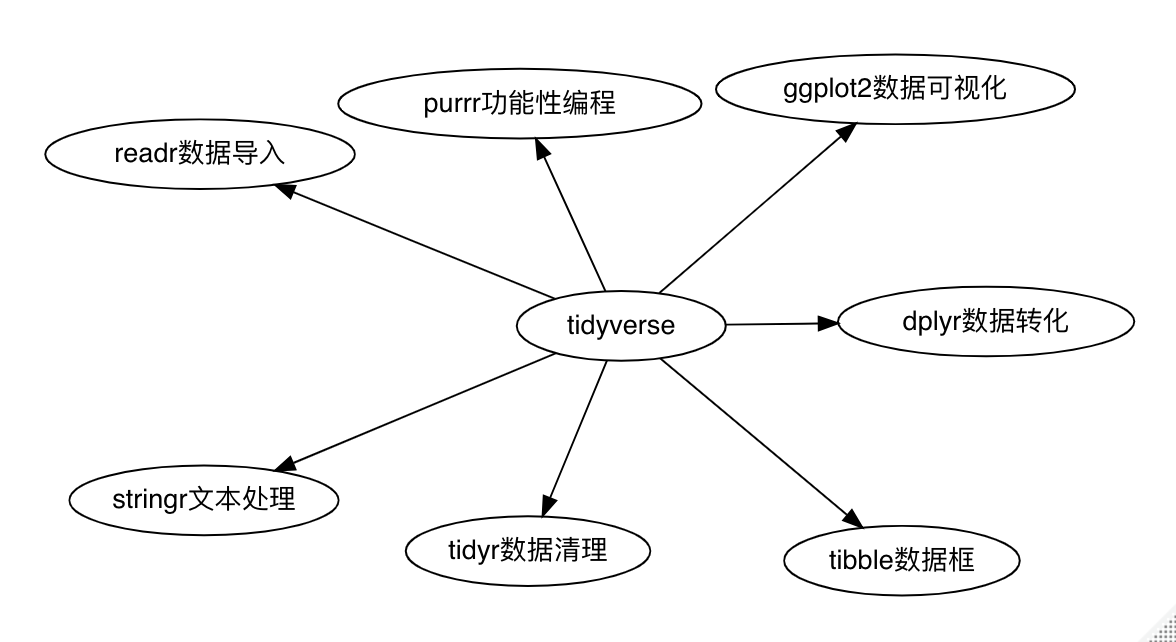
\includegraphics{images/fig3.1.png}
\caption{图1.1 Tidyverse系列工具包}
\end{figure}

首先,数据导入由readr完成。readr是一个用于读取数据的程序包,它能够快速有效地读取CSV、TSV和其他类型的文本文件。你可以使用read\_csv函数读取CSV文件(类似于使用R基础包中的read.csv函数)。
随后的数据整理(data wrangling)由dplyr和tidyr完成。其中dplyr侧重数据操纵,它提供了一系列函数,用于对数据集进行筛选、排序、修改和汇总等操作。tidyr侧重将数据转换成整洁数据(tidy data)的形式。
所谓``整洁数据''是指每个变量(variable)形成一列,每个观察(observation)形成一行,每个观测单元形成一张表)的形式组织数据。例如,你可以将宽格式的数据转换为长格式,或者将长格式的数据转换为宽格式。
对于字符串数据,stringr包,它提供了一系列简单易用的函数,用于处理字符串。例如,你可以使用str\_detect函数检测字符串中是否含有某个子串,或者用str\_replace函数替换字符串中的内容。

数据可视化由ggplot2包完成。ggplot2是一个基于图形语法(Grammar of Graphics)的设计理念而开发的强大且灵活的可视化工具。你可以使用ggplot2创建各种复杂的图形,如散点图、箱线图、直方图等,以展示数据分布、关系或比较差异等。

此外,purrr用于函数式编程的包,它提供了一系列高级工具,用于处理列表和函数。而tibble用于创建和操作tibble的包,tibble是一种现代化的数据框(data frame),比基础R的数据框更为优化。

这些包都被设计成能够很好地协同工作,并且它们的函数和语法都十分一致。这使得你可以将它们串联起来,形成一个数据科学工作流,包括数据的导入、整理、变换、可视化和模型拟合等步骤。tidyverse中所有这些包通过管道操作符(\%\textgreater{}\%)链接起来,使得数据分析的工作流程更加清晰和一致。例如,你可能先使用readr读取数据,然后用dplyr和tidyr进行数据清洗和转换,接着使用ggplot2进行可视化,最后使用purrr进行结果处理。此外,tidyverse生态系统还在不断扩展和改进,包括不断添加新的包和功能,以适应数据科学的新需求和挑战。

\hypertarget{ux7b2cux4e09ux7ae0-ux6570ux636eux79d1ux5b66ux57faux672cux6982ux5ff5}{%
\chapter{第三章 数据科学基本概念}\label{ux7b2cux4e09ux7ae0-ux6570ux636eux79d1ux5b66ux57faux672cux6982ux5ff5}}

\hypertarget{ux6570ux636eux7c7bux578b}{%
\section{数据类型}\label{ux6570ux636eux7c7bux578b}}

\hypertarget{ux7ed3ux6784ux578bux6570ux636eux548cux975eux7ed3ux6784ux578bux6570ux636e}{%
\subsection{结构型数据和非结构型数据}\label{ux7ed3ux6784ux578bux6570ux636eux548cux975eux7ed3ux6784ux578bux6570ux636e}}

根据数据的组织方式,数据科学中将数据分为结构型数据(Structured Data)和非结构型数据(Unstructured Data)。

结构型数据是指以明确定义的数据结构和数据模式组织的数据,其数据元素之间存在预定义的关系和属性,以便于存储、检索和分析。结构型数据具有固定的格式和字段,通常以表格、数据库、CSV(逗号分隔值)文件等形式存储。每个数据项都有预定义的类型,例如整数、浮点数、日期、文本等,且数据之间可以通过键值或主键进行关联。

非结构型数据是指没有固定格式和明确定义的数据,数据元素之间缺乏预定义的关系和属性,不易于直接存储和分析的数据形式。常见的非结构型数据有文本、图像、音频、视频等内容,其结构和含义需要进一步的处理和解析。这些数据通常存储在文档、图像文件、日志、社交媒体帖子等中。
示例:

\begin{itemize}
\tightlist
\item
  文本数据:社交媒体帖子、新闻文章、电子邮件等。
\item
  图像数据:照片、绘画、图表等。
\item
  音频数据:录音、音乐等。
\end{itemize}

在语言研究中,语言本体数据包括文本数据(含口语转录的文本)和语音数据。语言使用者的社会人口学数据也是语言研究的重要组成部分。在实验语言学或心理语言学研究中,数据还包括语言使用者加工语言的行为数据和神经活动数据。语言研究涉及的数据类型十分丰富,同时也为数据处理提出了巨大的挑战。

语言研究中,实验数据通常是结构性的。语音数据及标注,还有相应的声学指标,如时长,元音的共振峰,响音部分的基频等一般也是以结构性数据形式存在。结构化数据是较为容易存储,处理的。

文本数据比如博客,文章,小说等是非结构化的,不能直接用数据科学中的数据探索分析方法或者数据建模和数据可视化。文本数据可以通过分词,词频统计,特征提取等方法转化为结构性数据。只有当转化为结构性数据之后,进一步加入元数据,我们才能够来讨论变量之间的关系。在语言研究中,语料库数据通常是非结构性的,对语料库进行量化分析需要我们提取相应信息并转化成为结构性的数据。

\hypertarget{ux8d28ux6027ux6570ux636eux548cux91cfux5316ux6570ux636e}{%
\subsection{质性数据和量化数据}\label{ux8d28ux6027ux6570ux636eux548cux91cfux5316ux6570ux636e}}

根据数据的统计学特性,数据可以分为质性数据和量化数据。质性数据是指不能够用数字来表示,也不能够进行简单的数学计算,而仅仅用来描述某个事物的范畴属性。比如,语音学中一个音是元音,还是辅音。一个词的词性,名词,动词。一句话所具有的语用功能。
量化数据是可以用数字来描述并且可以进行简单的数学运算。进一步可以分为离散数据(Discrete)和连续数据( Continuous)。离散数据只能用某一些数值代表,比如参与实验的人数,实验中刺激的个数。连续数据( Continuous)可以有无限的数据数值代表,比如实验任务的反应时。

在科学研究中,为了探究一些问题,我们通过实验、调查、观察或其他数据收集方法获得的数据。数据通常用于描述和分析研究中的变量,并用于回答研究问题或测试假设。数据是对变量的测量或观察结果。

\hypertarget{ux6570ux636eux53d8ux91cf}{%
\section{数据变量}\label{ux6570ux636eux53d8ux91cf}}

变量是指任何可以被测量或计数的特征,用于描述不同个体或实物的特征,比如年龄、性别、企业收入和支出、出生国家、班级成绩、眼睛颜色和车辆类型都是常见的变量。变量之所以称为变量,是因为在一个总体(population)或数据集中,其值可能会在不同的个体之间有所变化,或者随着时间的推移可能会发生变化。例如,一个人的身高可以随着时间的推移而增长,一个企业的收入和支出可以随着季度或年份的变化而变化。

变量根据其描述性统计特性分为四种不同层次,分别为定类(nominal)、定序(ordinal)、定距及定比变量。定类和定序变量为类别变量(categorical),定距和定比变量为数值变量(numberic)。

\hypertarget{ux7c7bux522bux53d8ux91cf}{%
\subsubsection{类别变量}\label{ux7c7bux522bux53d8ux91cf}}

定性变量描述事物的``特征''、``类型''或``范畴'',通常使用非数字值表示。分类变量通常是排他的性,即一个个体属于同一变量中的一个类别。分类变量应该是详尽的,包括所有可能的类别。

类别变量可以进一步分为定类和定序两种。定类变量描述一个类别,无法按逻辑顺序进行组织。常见的该类变量包括性别、企业类型、眼睛颜色、宗教和品牌。我们可以描述其频数(率),或者一组数据中的众数 (出现频数最高的)。定序数据描述一个有顺序类别。比如,调查问卷中,喜欢、一般、厌恶,这3个选项就构成了有顺序数据。定序数据可以按数据顺序排列,因此除了众数之外,我们还可以描述其中位数,也就是将一组数据按一定顺序排列,其中处于中间位置的数据。定序变量的类别相互比较高低大小,但不一定能建立各个类别之间的数字差异。换句话说,变量水平之间的间隔是未知的。

在一些情况下,我们可以为有序变量的不同水平分配数字,实现定序变量转化为数值变量,但我们需要注意这些变量不是数值型的。例如,``非常同意''和``中立''不能平均为``同意'',即使我们将``非常同意''分配为5,将``中立''分配为3。

\hypertarget{ux6570ux503cux578bux53d8ux91cf}{%
\subsubsection{数值型变量}\label{ux6570ux503cux578bux53d8ux91cf}}

数值型变量描述了一个可测量的数量,其中数字之间的间隔是相等的。比如,1千克和2千克之间的间隔与3千克和4千克之间的间隔相等。
定距数据是一种数值性变量,一种具有等距间隔的变量,其中相邻数值之间的差异是相等的。比如气温。定距数据可以进行加减。定比数据和定距数据的区别在于,定比数据有一个零点。比如,年龄、体重、身高都属于定比数据,不存在负值。定比数据除了可以加减运算以外,还可以乘除运算。我们可以说一个人的年龄是另外一个人的两倍。

数值型变量可以进一步分为连续(continuous)变量和离散(discrete)变量两个子类。

离散变量由整数值组成,不能取介于两个值之间的值。常见的离散变量有:车辆数量、家庭子女数量。它们都以整数单位衡量。

连续变量可以取一定集合范围内任意一个值。连续变量的观测值可以包括仪器测量允许的最小值。连续变量的例子包括身高、时间、年龄和温度。

变量类型将决定(1)统计分析的方法;(2)我们如何使用统计数据和图表总结数据。

\begin{longtable}[]{@{}lllll@{}}
\toprule
数据层级 & 趋中性描述 & 变异性描述 & 数学运算 & 举例\tabularnewline
\midrule
\endhead
定类 & 众数 & 不能 & 是否相等,集合关系 & 实验反应选项、词性、语音类别\tabularnewline
定序 & 众数、中位数 & 不能 & 排序、比较 & 李克特量表问题数据\tabularnewline
定距 & 众数、中位数、算数平均值 & 极差、方差、标准差 & 加减 & 温度\tabularnewline
定比 & 众数、中位数、几何平均值 & 极差、方差、标准差 & 乘除 & 年龄、体重、身高\tabularnewline
\bottomrule
\end{longtable}

不同的变量需要以不同的数据类型存储在R中。名义变量和定序变量可以存储为字符类型(character)或因子(factors,具有级别)。数值型数据存储为数字,可以是整数(integer)、实数(real)、小数(decimal)。

一个数据集(dataset)可以包含一个或者多个变量,这些变量可能有一种或者多种不同的类型如果您只有一个变量,可以将其存储在向量中。然而,更常见的情况是您有一组需要存储或导入为矩阵或数据框的变量。

\hypertarget{ux6570ux636eux7ed3ux6784}{%
\section{数据结构}\label{ux6570ux636eux7ed3ux6784}}

在R中,基本的数据结构有向量(vector),数组(array),列表(list),数据框(data frame)和因子(factor)。

\hypertarget{ux5411ux91cfvector}{%
\subsection{向量(vector)}\label{ux5411ux91cfvector}}

向量是一种最基本的一维数据结构,可以包含相同类型的元素(data element)。可以通过使用c()函数创建向量,并且可以使用一系列基本函数索引、访问和修改向量中的元素。

\begin{Shaded}
\begin{Highlighting}[]
\CommentTok{#创建一个包含整数的向量}
\NormalTok{vector <-}\StringTok{ }\KeywordTok{c}\NormalTok{(}\DecValTok{1}\NormalTok{, }\DecValTok{2}\NormalTok{, }\DecValTok{3}\NormalTok{, }\DecValTok{4}\NormalTok{, }\DecValTok{5}\NormalTok{)}

\CommentTok{# 创建不同类型的向量}
\CommentTok{# 数值型}
\NormalTok{a =}\StringTok{ }\DecValTok{8}\OperatorTok{:}\DecValTok{17}

\NormalTok{b <-}\StringTok{ }\KeywordTok{c}\NormalTok{(}\DecValTok{9}\NormalTok{, }\DecValTok{10}\NormalTok{, }\DecValTok{100}\NormalTok{, }\DecValTok{38}\NormalTok{)}

\CommentTok{# 布尔型}
\NormalTok{c =}\StringTok{ }\KeywordTok{c}\NormalTok{ (}\OtherTok{TRUE}\NormalTok{, }\OtherTok{FALSE}\NormalTok{, }\OtherTok{TRUE}\NormalTok{, }\OtherTok{FALSE}\NormalTok{)}

\NormalTok{c =}\StringTok{ }\KeywordTok{c}\NormalTok{ (T, F, T, F)}

\CommentTok{# 字符型}
\NormalTok{d =}\StringTok{ }\KeywordTok{c}\NormalTok{ (}\StringTok{"TRUE"}\NormalTok{, }\StringTok{"FALSE"}\NormalTok{, }\StringTok{"FALSE"}\NormalTok{)}

\CommentTok{# 改变向量的类型}

\KeywordTok{as.vector}\NormalTok{(b, }\DataTypeTok{mode =} \StringTok{"character"}\NormalTok{)}
\end{Highlighting}
\end{Shaded}

值得注意的是,如果不同类型的数据被放入同一个向量,数据类型会发生改变。数值型数据会强制改变为字符型数据或布尔型数据。

\begin{Shaded}
\begin{Highlighting}[]
\NormalTok{e =}\StringTok{ }\KeywordTok{c}\NormalTok{(}\DecValTok{9}\NormalTok{,}\DecValTok{10}\NormalTok{, }\StringTok{"ab"}\NormalTok{, }\StringTok{"cd"}\NormalTok{)}

\NormalTok{f =}\StringTok{ }\KeywordTok{c}\NormalTok{(}\DecValTok{10}\NormalTok{, }\DecValTok{11}\NormalTok{, T, F)}
\end{Highlighting}
\end{Shaded}

除了单个输入之外,我们可以借助R语言的一些函数,批量生成向量中的元素。

\begin{Shaded}
\begin{Highlighting}[]
\NormalTok{A =}\StringTok{ }\DecValTok{9}\OperatorTok{:}\DecValTok{20} \OperatorTok{+}\StringTok{ }\DecValTok{1} \CommentTok{# A 是一个从9到20的向量,并且每个元素都加上了1。}

\NormalTok{B =}\StringTok{ }\KeywordTok{seq}\NormalTok{(}\DecValTok{1}\NormalTok{, }\DecValTok{10}\NormalTok{)}\CommentTok{# B 是一个从1到10的向量,其中的数字是连续的。}

\NormalTok{C =}\StringTok{ }\KeywordTok{seq}\NormalTok{(}\DecValTok{1}\NormalTok{, }\DecValTok{20}\NormalTok{, }\DataTypeTok{by =} \DecValTok{2}\NormalTok{)}\CommentTok{#C 是一个从1到20的向量,步长为2,也就是只包含奇数。}

\NormalTok{D =}\StringTok{ }\KeywordTok{rep}\NormalTok{(}\DecValTok{5}\NormalTok{, }\DecValTok{4}\NormalTok{)}\CommentTok{# D 是一个包含了4个5的向量。}

\NormalTok{E =}\StringTok{ }\KeywordTok{rep}\NormalTok{(}\KeywordTok{c}\NormalTok{(}\DecValTok{1}\NormalTok{, }\DecValTok{2}\NormalTok{, }\DecValTok{3}\NormalTok{), }\DecValTok{4}\NormalTok{)}\CommentTok{# E 是一个重复了4次的向量,其中包含了1、2、3这三个元素。}

\NormalTok{G =}\StringTok{ }\KeywordTok{rep}\NormalTok{(}\KeywordTok{c}\NormalTok{(}\DecValTok{1}\NormalTok{, }\DecValTok{2}\NormalTok{, }\DecValTok{3}\NormalTok{), }\DataTypeTok{each =} \DecValTok{4}\NormalTok{)}\CommentTok{# G 是一个重复了4次的向量,其中每个元素都重复了4次,即先重复1四次,然后重复2四次,最后重复3四次。}
\end{Highlighting}
\end{Shaded}

R语言中的一些基本函数,可以对包含不同类型数据的向量进行操作。

\begin{Shaded}
\begin{Highlighting}[]
\CommentTok{#length(): 返回向量的长度。}
\NormalTok{vector <-}\StringTok{ }\KeywordTok{c}\NormalTok{(}\DecValTok{1}\NormalTok{, }\DecValTok{2}\NormalTok{, }\DecValTok{3}\NormalTok{, }\DecValTok{4}\NormalTok{, }\DecValTok{5}\NormalTok{)}
\KeywordTok{length}\NormalTok{(vector)}

\CommentTok{# is.na(): 检查向量中是否存在缺失值(NA)。}
\NormalTok{vector<-}\StringTok{ }\KeywordTok{c}\NormalTok{(}\DecValTok{1}\NormalTok{, }\OtherTok{NA}\NormalTok{, }\DecValTok{3}\NormalTok{, }\OtherTok{NA}\NormalTok{, }\DecValTok{5}\NormalTok{)}
\KeywordTok{is.na}\NormalTok{(vector)}

\CommentTok{# which(): 返回满足条件的元素在向量中的索引。}
\NormalTok{vector<-}\StringTok{ }\KeywordTok{c}\NormalTok{(}\DecValTok{1}\NormalTok{, }\DecValTok{2}\NormalTok{, }\DecValTok{6}\NormalTok{, }\DecValTok{7}\NormalTok{, }\DecValTok{8}\NormalTok{)}
\KeywordTok{which}\NormalTok{(vector }\OperatorTok{>}\StringTok{ }\DecValTok{3}\NormalTok{)}

\CommentTok{# sample(): 随机从向量中抽取元素。可以用于实验随机抽样。}
\NormalTok{vector <-}\StringTok{ }\KeywordTok{c}\NormalTok{(}\DecValTok{1}\OperatorTok{:}\DecValTok{100}\NormalTok{)}
\KeywordTok{sample}\NormalTok{(vector, }\DataTypeTok{size =} \DecValTok{3}\NormalTok{)}
\end{Highlighting}
\end{Shaded}

针对数值型变量的向量

\begin{Shaded}
\begin{Highlighting}[]
\CommentTok{# sum(): 计算向量中所有元素的和。}
\NormalTok{vector <-}\StringTok{ }\KeywordTok{c}\NormalTok{(}\DecValTok{1}\OperatorTok{:}\DecValTok{50}\NormalTok{)}
\KeywordTok{sum}\NormalTok{(vector)}

\CommentTok{# mean(): 计算向量的平均值。}

\KeywordTok{mean}\NormalTok{(vector)}

\CommentTok{# median(): 计算向量的中位数。}

\KeywordTok{median}\NormalTok{(vector)}

\CommentTok{# min(): 返回向量中的最小值。}

\KeywordTok{min}\NormalTok{(vector)}

\CommentTok{# max(): 返回向量中的最大值。}

\KeywordTok{max}\NormalTok{(vector)}

\CommentTok{# sort(): 将向量中的元素按升序排序。}

\KeywordTok{sort}\NormalTok{(vector)}

\CommentTok{# rev(): 反转向量中元素的顺序。}

\KeywordTok{rev}\NormalTok{(vector)}

\CommentTok{# unique(): 返回向量中唯一的元素。}
\NormalTok{vector =}\StringTok{ }\KeywordTok{c}\NormalTok{(}\DecValTok{1}\NormalTok{,}\DecValTok{2}\NormalTok{,}\DecValTok{33}\NormalTok{,}\DecValTok{4}\NormalTok{,}\DecValTok{4}\NormalTok{,}\DecValTok{4}\NormalTok{,}\DecValTok{5}\NormalTok{,}\DecValTok{6}\NormalTok{,}\DecValTok{345}\NormalTok{)}
\KeywordTok{unique}\NormalTok{(vector)}

\CommentTok{# range(): 返回向量的取值范围(最小值和最大值)。}
\KeywordTok{range}\NormalTok{(vector )}

\KeywordTok{quantile}\NormalTok{(vector)}

\KeywordTok{round}\NormalTok{(}\KeywordTok{sd}\NormalTok{(vector), }\DecValTok{2}\NormalTok{)}
\end{Highlighting}
\end{Shaded}

针对字符串型变量

\begin{Shaded}
\begin{Highlighting}[]
\CommentTok{# paste(): 将向量中的元素连接为一个字符串。}
\NormalTok{vector <-}\StringTok{ }\KeywordTok{c}\NormalTok{(}\StringTok{"我"}\NormalTok{, }\StringTok{"爱"}\NormalTok{, }\StringTok{"XXX!"}\NormalTok{)}
\KeywordTok{paste}\NormalTok{(vector, }\DataTypeTok{collapse =} \StringTok{" "}\NormalTok{)}

\CommentTok{# tolower(): 转换向量中的字符为小写。}
\NormalTok{vector <-}\StringTok{ }\KeywordTok{c}\NormalTok{(}\StringTok{"HELLO"}\NormalTok{, }\StringTok{"WORLD"}\NormalTok{, }\StringTok{"!"}\NormalTok{)}
\KeywordTok{tolower}\NormalTok{(vector)}

\CommentTok{# toupper(): 转换向量中的字符为大写。}
\NormalTok{vector <-}\StringTok{ }\KeywordTok{c}\NormalTok{(}\StringTok{"hello"}\NormalTok{, }\StringTok{"world"}\NormalTok{, }\StringTok{"!"}\NormalTok{)}
\KeywordTok{toupper}\NormalTok{(vector)}

\CommentTok{# grep(): 在向量中搜索满足条件的模式,并返回其索引。}
\NormalTok{vector <-}\StringTok{ }\KeywordTok{c}\NormalTok{(}\StringTok{"苹果"}\NormalTok{, }\StringTok{"香蕉"}\NormalTok{, }\StringTok{"胡萝卜"}\NormalTok{, }\StringTok{"橙子"}\NormalTok{)}
\KeywordTok{grep}\NormalTok{(}\StringTok{"果"}\NormalTok{, vector)}
\end{Highlighting}
\end{Shaded}

\hypertarget{ux5217ux8868list}{%
\subsection{列表(list)}\label{ux5217ux8868list}}

列表是一种可以包含不同类型的元素的数据结构。列表可以使用list()函数创建,可以使用索引或元素名称来访问和修改列表中的元素。

\begin{Shaded}
\begin{Highlighting}[]
\CommentTok{# 创建一个包含整数、字符和向量的列表:}
\NormalTok{my_list <-}\StringTok{ }\KeywordTok{list}\NormalTok{(}\DecValTok{1}\NormalTok{, }\StringTok{"a"}\NormalTok{, }\KeywordTok{c}\NormalTok{(}\DecValTok{2}\NormalTok{, }\DecValTok{3}\NormalTok{, }\DecValTok{4}\NormalTok{))}

\NormalTok{my_list}
\end{Highlighting}
\end{Shaded}

列表的简单操作

\begin{Shaded}
\begin{Highlighting}[]
\CommentTok{# unlist() 函数:将list转换为向量。}
\NormalTok{my_list <-}\StringTok{ }\KeywordTok{list}\NormalTok{(}\StringTok{"apple"}\NormalTok{, }\StringTok{"banana"}\NormalTok{, }\StringTok{"orange"}\NormalTok{)}

\KeywordTok{unlist}\NormalTok{(my_list) }

\CommentTok{# lapply():对list中的每个元素应用一个函数。}
\NormalTok{my_list <-}\StringTok{ }\KeywordTok{list}\NormalTok{(}\DecValTok{1}\OperatorTok{:}\DecValTok{3}\NormalTok{, }\DecValTok{4}\OperatorTok{:}\DecValTok{6}\NormalTok{, }\DecValTok{7}\OperatorTok{:}\DecValTok{9}\NormalTok{)}

\KeywordTok{lapply}\NormalTok{(my_list, mean)}

\CommentTok{# sapply():对list中的每个元素应用一个函数,并将结果简化为向量。}
\NormalTok{my_list <-}\StringTok{ }\KeywordTok{list}\NormalTok{(}\DecValTok{1}\OperatorTok{:}\DecValTok{3}\NormalTok{, }\DecValTok{4}\OperatorTok{:}\DecValTok{6}\NormalTok{, }\DecValTok{7}\OperatorTok{:}\DecValTok{9}\NormalTok{)}
\KeywordTok{sapply}\NormalTok{(my_list, mean)}
\end{Highlighting}
\end{Shaded}

\hypertarget{ux77e9ux9635matrix}{%
\subsection{矩阵(matrix)}\label{ux77e9ux9635matrix}}

矩阵是一个二维数组,其中的所有元素都具有相同的模式(数字、字符或逻辑)。你可以通过matrix()函数来创建矩阵。

\begin{Shaded}
\begin{Highlighting}[]
\CommentTok{# 创建一个3行2列的矩阵:}

\NormalTok{data <-}\StringTok{ }\DecValTok{1}\OperatorTok{:}\DecValTok{6}
\NormalTok{matrix1 <-}\StringTok{ }\KeywordTok{matrix}\NormalTok{(data, }\DataTypeTok{nrow =} \DecValTok{3}\NormalTok{, }\DataTypeTok{ncol =} \DecValTok{2}\NormalTok{)}
\KeywordTok{print}\NormalTok{(matrix1)}
\end{Highlighting}
\end{Shaded}

在这个示例中,我们首先创建了一个从1到6的向量 data,然后我们创建了一个3行2列的矩阵 matrix1,并将这个向量的数据按列存入矩阵。输出的结果会是一个3行2列的矩阵,元素值按列从1到6。

在数据预处理阶段,我们可能需要将数据框转换为矩阵格式,以便于进行某些特定的数据处理或分析。例如,我们可以将数据框转换为矩阵,并进行归一化处理。很多机器学习算法(例如SVM、KNN等)在训练时,需要数据以矩阵的形式提供。其中的每一行对应一个观测值,每一列对应一个特征。

在文本分析中,我们经常会用到一个被称为``词频-文档矩阵''(Term Frequency - Document Matrix,简称TF-IDM)的结构,用来统计各个文档(例如文章、书籍等)中各个词语出现的频率。这个矩阵的每一行对应一个文档,每一列对应一个词语,矩阵中的每个元素表示对应词语在对应文档中出现的次数或频率。

首先,我们需要一个文档集。这里,我们将创建一个简单的文档集,包含3个文档:

\begin{Shaded}
\begin{Highlighting}[]
\NormalTok{documents <-}\StringTok{ }\KeywordTok{c}\NormalTok{(}\StringTok{"我 爱 数据 分析 。"}\NormalTok{,}
               \StringTok{"我 爱 编程 , 和 数据 分析"}\NormalTok{,}
               \StringTok{"我 是 数据 分析师"}\NormalTok{)}
\end{Highlighting}
\end{Shaded}

\begin{Shaded}
\begin{Highlighting}[]
\CommentTok{# install.packages("tm")}
\CommentTok{# library(tm)}
\CommentTok{# # 然后,我们创建一个文本文档向量,并对其进行预处理:}
\CommentTok{# }
\CommentTok{# docs <- Corpus(VectorSource(documents))}
\CommentTok{# docs <- tm_map(docs, content_transformer(tolower))}
\CommentTok{# docs <- tm_map(docs, removePunctuation)}
\CommentTok{# docs <- tm_map(docs, removeNumbers)}
\CommentTok{# docs <- tm_map(docs, removeWords, stopwords("english"))}
\CommentTok{# docs <- tm_map(docs, stripWhitespace)}
\end{Highlighting}
\end{Shaded}

在这里,我们首先用Corpus()和VectorSource()函数来创建一个文档库。然后,我们用tm\_map()函数和各种预处理函数来对文档进行预处理,包括转换为小写、移除标点符号、移除数字、移除停用词和移除多余的空白字符。

最后,我们可以用DocumentTermMatrix()函数来创建一个词频-文档矩阵:

\begin{Shaded}
\begin{Highlighting}[]
\CommentTok{# dtm <- DocumentTermMatrix(docs)}
\CommentTok{# print(dtm)}
\end{Highlighting}
\end{Shaded}

这样,我们就创建了一个词频-文档矩阵,其中的每一行对应一个文档,每一列对应一个词语,矩阵中的每个元素表示对应词语在对应文档中出现的次数。后面可以用这个词频-文档矩阵来进行后续的文本分析,例如主题模型、文档分类、文档相似度计算等。

\hypertarget{ux6570ux636eux6846data-frame}{%
\subsection{数据框(data frame)}\label{ux6570ux636eux6846data-frame}}

数据框是一种表格形式的数据结构,类似于数据库的表格。数据框可以包含不同类型的列,并且每列的长度必须相同。数据框可以使用data.frame()函数创建,并可以使用列名称或索引来访问和修改数据框中的数据。

例如,创建一个包含姓名和年龄的数据框:

\begin{Shaded}
\begin{Highlighting}[]
\CommentTok{# 创建一个数据框}
\NormalTok{df <-}\StringTok{ }\KeywordTok{data.frame}\NormalTok{(}
  \DataTypeTok{name =} \KeywordTok{c}\NormalTok{(}\StringTok{"John"}\NormalTok{, }\StringTok{"Mary"}\NormalTok{, }\StringTok{"Peter"}\NormalTok{),}
  \DataTypeTok{age =} \KeywordTok{c}\NormalTok{(}\DecValTok{25}\NormalTok{, }\DecValTok{32}\NormalTok{, }\DecValTok{45}\NormalTok{),}
  \DataTypeTok{gender =} \KeywordTok{c}\NormalTok{(}\StringTok{"Male"}\NormalTok{, }\StringTok{"Female"}\NormalTok{, }\StringTok{"Male"}\NormalTok{)}
\NormalTok{)}
\end{Highlighting}
\end{Shaded}

\begin{Shaded}
\begin{Highlighting}[]
\CommentTok{# summary():用于查看数据框的统计信息。}
\KeywordTok{summary}\NormalTok{(df) }\CommentTok{#(输出df的基本统计信息,包括均值、中位数、最大值、最小值等。)}
\end{Highlighting}
\end{Shaded}

对于字符类型(如 name 和 gender),summary() 函数会显示变量长度。

对于数值类型(如 age),summary() 函数会显示最小值(Min.)、第一四分位数(1st Qu.)、中位数(Median)、平均值(Mean)、第三四分位数(3rd Qu.)和最大值(Max.)。

\begin{Shaded}
\begin{Highlighting}[]
\CommentTok{# 查看数据框的结构}
\KeywordTok{str}\NormalTok{(df)}
\end{Highlighting}
\end{Shaded}

\begin{verbatim}
## 'data.frame':    3 obs. of  3 variables:
##  $ name  : chr  "John" "Mary" "Peter"
##  $ age   : num  25 32 45
##  $ gender: chr  "Male" "Female" "Male"
\end{verbatim}

在输出结果中,以下是每一部分的含义:

\begin{itemize}
\item
  `data.frame':这是 df 的数据类型,即数据框(data frame)。
\item
  3 obs. of 3 variables:这表示 df 有3个观察值(即行)和3个变量(即列)。
\end{itemize}

接下来的部分列出了数据框的每一个变量(列):

\begin{itemize}
\item
  name : chr ``John'' ``Mary'' ``Peter'': name 表示 df 的一个变量是 name,: chr 表示 name 变量的数据类型是字符型 (character),接着的 ``John'' ``Mary'' ``Peter'' 是 name 变量的前几个观察值。
\item
  age : num 25 32 45:age 表示 df 的另一个变量是 age,: num 表示 age 变量的数据类型是数值型 (numeric),接着的 25 32 45 是 age 变量的前几个观察值。
\item
  gender: chr ``Male'' ``Female'' ``Male'':gender 表示 df 的另一个变量是 gender,: chr 表示 gender 变量的数据类型是字符型 (character),接着的 ``Male'' ``Female'' ``Male'' 是 gender 变量的前几个观察值。
\end{itemize}

\begin{Shaded}
\begin{Highlighting}[]
\CommentTok{# nrow():用于计算数据框的行数。}
\KeywordTok{nrow}\NormalTok{(df) }\CommentTok{#(输出df的行数。)}

\CommentTok{# ncol():用于计算数据框的列数。}
\KeywordTok{ncol}\NormalTok{(df) }\CommentTok{#(输出df的列数。)}

\CommentTok{# head():用于查看数据框的前几行数据。}
\KeywordTok{head}\NormalTok{(df, }\DataTypeTok{n =} \DecValTok{2}\NormalTok{) }\CommentTok{#(输出df的前10行数据。)}

\CommentTok{# tail():用于查看数据框的后几行数据。}
\KeywordTok{tail}\NormalTok{(df, }\DataTypeTok{n =} \DecValTok{2}\NormalTok{) }\CommentTok{#(输出df的后5行数据。)}

\CommentTok{# unique():用于去重并输出数据框中唯一的值。}
\KeywordTok{unique}\NormalTok{(df}\OperatorTok{$}\NormalTok{gender) }\CommentTok{#(输出df中gender列的唯一值。)}
\end{Highlighting}
\end{Shaded}

在词频-文档矩阵(TF-IDM)的例子中,我们不能使用数据框(data frame)作为数据结构,原因主要有两个:

\begin{itemize}
\item
  稀疏性:在文本分析中,词频-文档矩阵通常非常稀疏,也就是说,矩阵中的大部分元素都是零(因为每个文档只包含词汇表中的一小部分词语)。而在R中,数据框不支持稀疏数据,如果我们尝试将一个大的稀疏矩阵存储为数据框,那么它将占用大量的内存。相反,词频-文档矩阵通常以稀疏矩阵的形式存储,这种格式只存储非零元素,从而大大节省了内存。
\item
  矩阵运算:在文本分析中,我们经常需要对词频-文档矩阵进行各种矩阵运算,例如矩阵乘法、转置等。在R中,数据框不支持这些矩阵运算,如果我们尝试对数据框执行这些操作,那么我们需要先将其转换为矩阵。而如果我们直接使用矩阵来存储数据,那么我们可以直接执行这些操作,无需进行类型转换。
\end{itemize}

综上,尽管数据框是R中最常用的数据结构,但在处理文本数据时,使用词频-文档矩阵(以及更一般的稀疏矩阵)通常更为方便和高效。

\hypertarget{ux6570ux7ec4array}{%
\subsection{数组(array)}\label{ux6570ux7ec4array}}

数组是一个可以存储具有相同数据类型元素的多维数据结构。可以使用array()函数创建数组。

\begin{Shaded}
\begin{Highlighting}[]
\CommentTok{# 创建一个一维数组:}
\NormalTok{data <-}\StringTok{ }\DecValTok{1}\OperatorTok{:}\DecValTok{10}
\NormalTok{array1 <-}\StringTok{ }\KeywordTok{array}\NormalTok{(data, }\DataTypeTok{dim =} \KeywordTok{c}\NormalTok{(}\DecValTok{10}\NormalTok{))}
\KeywordTok{print}\NormalTok{(array1)}
\CommentTok{# 在这个示例中,我们首先创建了一个从1到10的向量 data,然后我们创建了一个一维数组 array1,并将这个向量的数据存入数组。输出的结果会是1到10的一维数组。}

\CommentTok{# 创建一个二维数组:}
\NormalTok{data <-}\StringTok{ }\DecValTok{1}\OperatorTok{:}\DecValTok{12}
\NormalTok{array2 <-}\StringTok{ }\KeywordTok{array}\NormalTok{(data, }\DataTypeTok{dim =} \KeywordTok{c}\NormalTok{(}\DecValTok{3}\NormalTok{, }\DecValTok{4}\NormalTok{))}
\KeywordTok{print}\NormalTok{(array2)}
\CommentTok{# 在这个示例中,我们创建了一个二维数组 array2,它有3行4列。输出的结果会是一个3行4列的二维数组,元素值从1到12。}

\CommentTok{# 创建一个三维数组:}
\NormalTok{data <-}\StringTok{ }\DecValTok{1}\OperatorTok{:}\DecValTok{24}
\NormalTok{array3 <-}\StringTok{ }\KeywordTok{array}\NormalTok{(data, }\DataTypeTok{dim =} \KeywordTok{c}\NormalTok{(}\DecValTok{2}\NormalTok{, }\DecValTok{3}\NormalTok{, }\DecValTok{4}\NormalTok{))}
\KeywordTok{print}\NormalTok{(array3)}
\CommentTok{# 在这个示例中,我们创建了一个三维数组 array3,它有2个2行3列的面。输出的结果会是一个2行3列,共有2个面的三维数组,元素值从1到24。}
\end{Highlighting}
\end{Shaded}

在数据科学实践中,尽管数组可能不如数据框或列表那么常用,但它们在某些特定的情况下是非常有用的。例如,当数据自然地以多维形式出现时,数组可以是理想的数据结构。例如,如果在不同时间、不同地点收集到了大气温度数据,你可以将这些数据存储在一个三维数组中,其中一个维度代表时间,另一个维度代表经度,第三个维度代表纬度。在这种情况下,使用数组可以使数据的处理和分析更加直观和方便。

\begin{longtable}[]{@{}lll@{}}
\toprule
Dimensions & Homogenous & Heterogeneous\tabularnewline
\midrule
\endhead
1D & Vector & List\tabularnewline
2D & Matrix & Data frame\tabularnewline
nD & Array &\tabularnewline
\bottomrule
\end{longtable}

在R语言中,有五种主要的数据结构:向量(vector)、矩阵(matrix)、数组(array)、列表(list)和数据框(data frame)。这些数据结构是R编程中非常常用的,可以帮助我们有效地组织和处理数据。每种数据结构都有其特定的用途,适用于处理不同类型和维度的数据。

向量是最基础的数据结构,它是一维的,只包含同类元素,即所有元素的数据类型必须相同。在数据科学中,向量通常用于存储数值、字符或逻辑数据。

矩阵是二维的数据结构,其中的所有元素必须具有相同的数据类型。它适用于需要在两个维度上组织数据的情况,例如在文本分析中创建一个词频矩阵。

数组可以是多维的,其中的所有元素必须具有相同的数据类型。当需要在三个或更多的维度上组织数据时,可以使用数组。例如,在图像处理中,可以用一个三维数组来表示一张彩色图像,其中的每个元素表示一个像素的红、绿或蓝色分量。

列表是一种异质的数据结构,它可以包含不同类型的元素,包括向量、矩阵、数组、列表等。当需要在一个对象中存储异质的数据时,可以使用列表。典型例子:在建立回归模型后,可以将结果存储在一个列表中。

\begin{Shaded}
\begin{Highlighting}[]
\CommentTok{# 这行代码使用R中的lm()函数(线性模型)来拟合一个线性回归模型。模型的目标(因变量)是mpg(每加仑英里数),预测变量(自变量)是hp(马力)。数据源是R自带的mtcars数据集。}
\NormalTok{model <-}\StringTok{ }\KeywordTok{lm}\NormalTok{(mpg }\OperatorTok{~}\StringTok{ }\NormalTok{hp, }\DataTypeTok{data =}\NormalTok{ mtcars)}
\CommentTok{# 这行代码创建一个列表,其中包含了线性模型的系数(coefficients)、残差(residuals)和拟合值(fitted.values)。}
\NormalTok{model_summary <-}\StringTok{ }\KeywordTok{list}\NormalTok{(}\DataTypeTok{coefficients =}\NormalTok{ model}\OperatorTok{$}\NormalTok{coefficients, }
                      \DataTypeTok{residuals =}\NormalTok{ model}\OperatorTok{$}\NormalTok{residuals, }
                      \DataTypeTok{fitted.values =}\NormalTok{ model}\OperatorTok{$}\NormalTok{fitted.values)}
\CommentTok{#这行代码返回并打印model_summary列表的内容。}
\NormalTok{model_summary}
\end{Highlighting}
\end{Shaded}

数据框是二维的数据结构,每一列是一个向量,可以是不同的数据类型,但每一行必须具有相同的长度。在数据科学中,数据框通常用于存储数据表。

\hypertarget{ux7b2cux56dbux7ae0-ux6570ux636eux52a0ux5de5}{%
\chapter{第四章 数据加工}\label{ux7b2cux56dbux7ae0-ux6570ux636eux52a0ux5de5}}

\hypertarget{ux6570ux636eux9884ux5904ux7406}{%
\section{数据预处理}\label{ux6570ux636eux9884ux5904ux7406}}

数据预处理主要是指在进行数据分析和建模之前,对原始数据进行一系列的处理步骤,以确保数据的质量和准确性,消除数据中的噪声和错误,以及为后续的分析和建模做好准备。数据预处理的步骤包括数据清理(Data Cleaning)、数据转换(Data Transformation)、数据集成(Data Integration)和数据规约(Data Reduction)等。

\hypertarget{ux6570ux636eux6e05ux7406}{%
\subsection{数据清理}\label{ux6570ux636eux6e05ux7406}}

数据清理(Data Cleaning)是数据科学和数据分析中的重要步骤,指的是对原始数据进行检查、修正和转换,以确保数据质量和准确性,使数据更适合后续的分析和建模工作。数据清理是数据预处理过程中的关键环节,它的目标是处理数据中的错误、缺失、异常和重复值等问题,从而得到干净、可靠的数据集。
解决数据类型问题:确保数据类型正确,例如将数值型数据转换为数字类型,将日期数据转换为日期类型等。
数据合并:如果数据来自不同的源头,可能需要将多个数据集合并成一个整体数据集,进行数据整合和关联分析。

\begin{Shaded}
\begin{Highlighting}[]
\KeywordTok{library}\NormalTok{(tidyverse)}
\CommentTok{# 创建含有错误值的数据}
\KeywordTok{set.seed}\NormalTok{(}\DecValTok{123}\NormalTok{)  }\CommentTok{# 设置随机种子以确保可重复性}
\NormalTok{df_errors <-}\StringTok{ }\KeywordTok{data.frame}\NormalTok{(}\DataTypeTok{Student_ID =} \DecValTok{1}\OperatorTok{:}\DecValTok{100}\NormalTok{,}
                    \DataTypeTok{Listening_Score =} \KeywordTok{sample}\NormalTok{(}\OperatorTok{-}\DecValTok{5}\OperatorTok{:}\DecValTok{100}\NormalTok{, }\DecValTok{100}\NormalTok{, }\DataTypeTok{replace =} \OtherTok{TRUE}\NormalTok{),}
                    \DataTypeTok{Speaking_Score =} \KeywordTok{sample}\NormalTok{(}\DecValTok{0}\OperatorTok{:}\DecValTok{999}\NormalTok{, }\DecValTok{100}\NormalTok{, }\DataTypeTok{replace =} \OtherTok{TRUE}\NormalTok{),}
                    \DataTypeTok{Reading_Score =} \KeywordTok{sample}\NormalTok{(}\DecValTok{0}\OperatorTok{:}\DecValTok{105}\NormalTok{, }\DecValTok{100}\NormalTok{, }\DataTypeTok{replace =} \OtherTok{TRUE}\NormalTok{),}
                    \DataTypeTok{Writing_Score =} \KeywordTok{sample}\NormalTok{(}\DecValTok{0}\OperatorTok{:}\DecValTok{100}\NormalTok{, }\DecValTok{100}\NormalTok{, }\DataTypeTok{replace =} \OtherTok{TRUE}\NormalTok{),}
                    \DataTypeTok{Age =} \KeywordTok{sample}\NormalTok{(}\DecValTok{18}\OperatorTok{:}\DecValTok{250}\NormalTok{, }\DecValTok{100}\NormalTok{, }\DataTypeTok{replace =} \OtherTok{TRUE}\NormalTok{),}
                    \DataTypeTok{Gender =} \KeywordTok{sample}\NormalTok{(}\KeywordTok{c}\NormalTok{(}\StringTok{"Male"}\NormalTok{, }\StringTok{"Female"}\NormalTok{), }\DecValTok{100}\NormalTok{, }\DataTypeTok{replace =} \OtherTok{TRUE}\NormalTok{))}
\end{Highlighting}
\end{Shaded}

\begin{infobox}task
任务1
- 对数据进行初步观察,了解数据的结构、特点和问题。
- 查看数据的前几行、数据类型、统计摘要等。

\end{infobox}

\begin{infobox}task
任务2 处理异常值
异常值是指与其他观测值明显不同的异常点,可能是数据录入错误或者异常情况。可以选择删除异常值或者采用合适的方法进行处理。
-学生听力分数为-5分,这是一个错误值。
-学生阅读分数超过满分100分,这是一个错误值。

\end{infobox}

\begin{Shaded}
\begin{Highlighting}[]
\CommentTok{# 使用if_else函数将错误值替换为NA}
\NormalTok{df_errors }\OperatorTok\StringTok{ }
\StringTok{  }\KeywordTok{filter}\NormalTok{(Listening_Score }\OperatorTok{<}\StringTok{ }\DecValTok{0} \OperatorTok{|}\StringTok{ }\NormalTok{Reading_Score }\OperatorTok{>}\StringTok{ }\DecValTok{100}\NormalTok{)}
\end{Highlighting}
\end{Shaded}

\begin{verbatim}
##   Student_ID Listening_Score Speaking_Score Reading_Score Writing_Score Age Gender
## 1         51              87            788           104            93  70 Female
## 2         59              85             38           105            92  87 Female
## 3         80              -2            309            34            41 185 Female
## 4        100              90            596           104            18 184   Male
\end{verbatim}

\begin{infobox}task
任务3 处理缺失值
处理缺失值是数据清理的重要一环。可以选择删除包含缺失值的样本、进行插补,或者使用特定方法填补缺失值。

\end{infobox}

\begin{Shaded}
\begin{Highlighting}[]
\CommentTok{# 创建含有缺失值的数据}
\KeywordTok{set.seed}\NormalTok{(}\DecValTok{123}\NormalTok{)  }\CommentTok{# 设置随机种子以确保可重复性}
\NormalTok{df_missing <-}\StringTok{ }\KeywordTok{tibble}\NormalTok{(}\DataTypeTok{Student_ID =} \DecValTok{1}\OperatorTok{:}\DecValTok{100}\NormalTok{,}
                     \DataTypeTok{Listening_Score =} \KeywordTok{sample}\NormalTok{(}\DecValTok{0}\OperatorTok{:}\DecValTok{999}\NormalTok{, }\DecValTok{100}\NormalTok{, }\DataTypeTok{replace =} \OtherTok{TRUE}\NormalTok{),}
                     \DataTypeTok{Speaking_Score =} \KeywordTok{sample}\NormalTok{(}\DecValTok{0}\OperatorTok{:}\DecValTok{100}\NormalTok{, }\DecValTok{100}\NormalTok{, }\DataTypeTok{replace =} \OtherTok{TRUE}\NormalTok{),}
                     \DataTypeTok{Reading_Score =} \KeywordTok{sample}\NormalTok{(}\DecValTok{0}\OperatorTok{:}\DecValTok{100}\NormalTok{, }\DecValTok{100}\NormalTok{, }\DataTypeTok{replace =} \OtherTok{TRUE}\NormalTok{),}
                     \DataTypeTok{Writing_Score =} \KeywordTok{sample}\NormalTok{(}\DecValTok{0}\OperatorTok{:}\DecValTok{100}\NormalTok{, }\DecValTok{100}\NormalTok{, }\DataTypeTok{replace =} \OtherTok{TRUE}\NormalTok{),}
                     \DataTypeTok{Age =} \KeywordTok{sample}\NormalTok{(}\KeywordTok{c}\NormalTok{(}\DecValTok{18}\OperatorTok{:}\DecValTok{40}\NormalTok{, }\OtherTok{NA}\NormalTok{), }\DecValTok{100}\NormalTok{, }\DataTypeTok{replace =} \OtherTok{TRUE}\NormalTok{),}
                     \DataTypeTok{Gender =} \KeywordTok{sample}\NormalTok{(}\KeywordTok{c}\NormalTok{(}\StringTok{"Male"}\NormalTok{, }\StringTok{"Female"}\NormalTok{), }\DecValTok{100}\NormalTok{, }\DataTypeTok{replace =} \OtherTok{TRUE}\NormalTok{))}

\CommentTok{# 使用complete函数删除包含缺失值的样本}
\NormalTok{df_missing2 <-}\StringTok{ }\NormalTok{df_missing }\OperatorTok\StringTok{ }
\StringTok{  }\KeywordTok{na.omit}\NormalTok{()}
\end{Highlighting}
\end{Shaded}

\begin{infobox}task
任务4 处理重复值:重复值是指在数据集中出现多次的相同观测值。需要检查并删除重复值,确保每个观测只出现一次。
-学生听力分数和口语分数中有重复的记录。
-学生年龄和性别中有重复的记录。

\end{infobox}

\begin{Shaded}
\begin{Highlighting}[]
\CommentTok{# 创建含有重复值的数据}
\KeywordTok{set.seed}\NormalTok{(}\DecValTok{123}\NormalTok{)  }\CommentTok{# 设置随机种子以确保可重复性}
\NormalTok{df_duplicates <-}\StringTok{ }\KeywordTok{tibble}\NormalTok{(}\DataTypeTok{Student_ID =} \KeywordTok{rep}\NormalTok{(}\DecValTok{1}\OperatorTok{:}\DecValTok{50}\NormalTok{, }\DataTypeTok{each =} \DecValTok{2}\NormalTok{),}
                        \DataTypeTok{Listening_Score =} \KeywordTok{sample}\NormalTok{(}\DecValTok{0}\OperatorTok{:}\DecValTok{100}\NormalTok{, }\DecValTok{100}\NormalTok{, }\DataTypeTok{replace =} \OtherTok{TRUE}\NormalTok{),}
                        \DataTypeTok{Speaking_Score =} \KeywordTok{sample}\NormalTok{(}\DecValTok{0}\OperatorTok{:}\DecValTok{100}\NormalTok{, }\DecValTok{100}\NormalTok{, }\DataTypeTok{replace =} \OtherTok{TRUE}\NormalTok{),}
                        \DataTypeTok{Reading_Score =} \KeywordTok{sample}\NormalTok{(}\DecValTok{0}\OperatorTok{:}\DecValTok{100}\NormalTok{, }\DecValTok{100}\NormalTok{, }\DataTypeTok{replace =} \OtherTok{TRUE}\NormalTok{),}
                        \DataTypeTok{Writing_Score =} \KeywordTok{sample}\NormalTok{(}\DecValTok{0}\OperatorTok{:}\DecValTok{100}\NormalTok{, }\DecValTok{100}\NormalTok{, }\DataTypeTok{replace =} \OtherTok{TRUE}\NormalTok{),}
                        \DataTypeTok{Age =} \KeywordTok{sample}\NormalTok{(}\KeywordTok{c}\NormalTok{(}\DecValTok{18}\OperatorTok{:}\DecValTok{25}\NormalTok{), }\DecValTok{100}\NormalTok{, }\DataTypeTok{replace =} \OtherTok{TRUE}\NormalTok{),}
                        \DataTypeTok{Gender =} \KeywordTok{sample}\NormalTok{(}\KeywordTok{c}\NormalTok{(}\StringTok{"Male"}\NormalTok{, }\StringTok{"Female"}\NormalTok{), }\DecValTok{100}\NormalTok{, }\DataTypeTok{replace =} \OtherTok{TRUE}\NormalTok{))}

\CommentTok{# 使用duplicated函数删除重复值}
\NormalTok{df_duplicates <-}\StringTok{ }\NormalTok{df_duplicates }\OperatorTok\StringTok{ }
\StringTok{  }\KeywordTok{filter}\NormalTok{(}\OperatorTok{!}\KeywordTok{duplicated}\NormalTok{(Student_ID))}
\end{Highlighting}
\end{Shaded}

\begin{infobox}task
任务5

\end{infobox}

\hypertarget{ux6570ux636eux8f6cux6362}{%
\subsection{数据转换}\label{ux6570ux636eux8f6cux6362}}

数据转换(Data Transformation)是数据处理中的一个重要环节,指的是对原始数据进行变换、重构或调整,以使数据更适合分析和建模。数据转换的目的是为了改变数据的结构和特征,以满足数据分析的需求和假设。

数据转换可以包括特征工程(Feature Engineering)、数据标准化(Data Standardization)、数据归一化(Data Normalization)、对数化(Logarithm)、聚合(Aggregation)等操作。

特征构造(Feature Construction):基于已有的特征构造新的特征,以提供更有用的信息。

\begin{itemize}
\item
  数据标准化(Data Standardization):将不同特征的数据缩放到相同的尺度,消除特征之间的量纲差异。
\item
  数据归一化(Data Normalization):将数据缩放到{[}0, 1{]}范围内,使得不同特征的权重相同。
\item
  对数化(Logarithm):将数据进行对数变换,使得数据更加符合线性关系或满足某些假设。
\end{itemize}

数据聚合(Aggregation):将数据进行聚合操作,例如求和、求平均等。

数据拆分(Data Splitting):将数据按照一定的规则拆分成多个子数据集,用于特定的分析需求。

数据清理和数据转换是数据预处理的两个重要环节,它们之间有一些区别:

\begin{itemize}
\item
  目的不同:数据清理的目的是处理数据中的错误、缺失、异常和重复值等问题,保证数据的质量和准确性;而数据转换的目的是改变数据的结构和特征,以满足数据分析和建模的需求。
\item
  内容不同:数据清理主要关注数据本身的质量问题,包括缺失值(Missing Values)、异常值(Outliers)等;而数据转换主要关注如何更好地表达数据、提取特征、消除量纲差异等。
\item
  操作不同:数据清理的操作主要包括删除(Deletion)、填补(Imputation)、修正(Correction)等;而数据转换的操作主要包括缩放(Scaling)、标准化(Standardization)、对数化(Logarithm)、聚合(Aggregation)等。
\end{itemize}

\begin{infobox}task
任务5

我们创建一个包含200个真实汉语词汇的数据集,包含词频、抽象度、意象度、词汇起始习得年龄、词汇难度、词汇情感评分等变量。

\end{infobox}

\begin{Shaded}
\begin{Highlighting}[]
\CommentTok{# 创建含有真实汉语词汇的数据集}
\KeywordTok{set.seed}\NormalTok{(}\DecValTok{123}\NormalTok{)  }\CommentTok{# 设置随机种子以确保可重复性}
\NormalTok{df_vocabulary <-}\StringTok{ }\KeywordTok{data.frame}\NormalTok{(}\DataTypeTok{Word =} \KeywordTok{c}\NormalTok{(}\StringTok{"苹果"}\NormalTok{, }\StringTok{"梨子"}\NormalTok{, }\StringTok{"香蕉"}\NormalTok{, }\StringTok{"草莓"}\NormalTok{, }\StringTok{"桃子"}\NormalTok{, }\StringTok{"西瓜"}\NormalTok{, }\StringTok{"橙子"}\NormalTok{, }\StringTok{"柚子"}\NormalTok{, }\StringTok{"葡萄"}\NormalTok{, }\StringTok{"芒果"}\NormalTok{,}
                                 \StringTok{"书"}\NormalTok{, }\StringTok{"笔"}\NormalTok{, }\StringTok{"课本"}\NormalTok{, }\StringTok{"教室"}\NormalTok{, }\StringTok{"黑板"}\NormalTok{, }\StringTok{"学生"}\NormalTok{, }\StringTok{"老师"}\NormalTok{, }\StringTok{"考试"}\NormalTok{, }\StringTok{"作业"}\NormalTok{, }\StringTok{"校园"}\NormalTok{,}
                                 \StringTok{"美食"}\NormalTok{, }\StringTok{"旅游"}\NormalTok{, }\StringTok{"音乐"}\NormalTok{, }\StringTok{"电影"}\NormalTok{, }\StringTok{"运动"}\NormalTok{, }\StringTok{"阅读"}\NormalTok{, }\StringTok{"绘画"}\NormalTok{, }\StringTok{"写作"}\NormalTok{, }\StringTok{"摄影"}\NormalTok{, }\StringTok{"游戏"}\NormalTok{,}
                                 \StringTok{"猫"}\NormalTok{, }\StringTok{"狗"}\NormalTok{, }\StringTok{"兔子"}\NormalTok{, }\StringTok{"鱼"}\NormalTok{, }\StringTok{"鸟"}\NormalTok{, }\StringTok{"大象"}\NormalTok{, }\StringTok{"狮子"}\NormalTok{, }\StringTok{"熊猫"}\NormalTok{, }\StringTok{"猴子"}\NormalTok{, }\StringTok{"蛇"}\NormalTok{,}
                                 \StringTok{"早晨"}\NormalTok{, }\StringTok{"中午"}\NormalTok{, }\StringTok{"下午"}\NormalTok{, }\StringTok{"晚上"}\NormalTok{, }\StringTok{"春天"}\NormalTok{, }\StringTok{"夏天"}\NormalTok{, }\StringTok{"秋天"}\NormalTok{, }\StringTok{"冬天"}\NormalTok{, }\StringTok{"天气"}\NormalTok{, }\StringTok{"季节"}\NormalTok{,}
                                 \StringTok{"篮球"}\NormalTok{, }\StringTok{"足球"}\NormalTok{, }\StringTok{"乒乓球"}\NormalTok{, }\StringTok{"网球"}\NormalTok{, }\StringTok{"羽毛球"}\NormalTok{, }\StringTok{"游泳"}\NormalTok{, }\StringTok{"滑雪"}\NormalTok{, }\StringTok{"跑步"}\NormalTok{, }\StringTok{"健身"}\NormalTok{, }\StringTok{"瑜伽"}\NormalTok{),}
                        \DataTypeTok{Frequency =} \KeywordTok{sample}\NormalTok{(}\DecValTok{1}\OperatorTok{:}\DecValTok{1000}\NormalTok{, }\DecValTok{60}\NormalTok{, }\DataTypeTok{replace =} \OtherTok{TRUE}\NormalTok{),}
                        \DataTypeTok{Abstractness =} \KeywordTok{sample}\NormalTok{(}\DecValTok{1}\OperatorTok{:}\DecValTok{5}\NormalTok{, }\DecValTok{60}\NormalTok{, }\DataTypeTok{replace =} \OtherTok{TRUE}\NormalTok{),}
                        \DataTypeTok{Imagery =} \KeywordTok{sample}\NormalTok{(}\DecValTok{1}\OperatorTok{:}\DecValTok{5}\NormalTok{, }\DecValTok{60}\NormalTok{, }\DataTypeTok{replace =} \OtherTok{TRUE}\NormalTok{),}
                        \DataTypeTok{Age_of_Acquisition =} \KeywordTok{sample}\NormalTok{(}\DecValTok{3}\OperatorTok{:}\DecValTok{12}\NormalTok{, }\DecValTok{60}\NormalTok{, }\DataTypeTok{replace =} \OtherTok{TRUE}\NormalTok{),}
                        \DataTypeTok{Difficulty =} \KeywordTok{sample}\NormalTok{(}\DecValTok{1}\OperatorTok{:}\DecValTok{5}\NormalTok{, }\DecValTok{60}\NormalTok{, }\DataTypeTok{replace =} \OtherTok{TRUE}\NormalTok{),}
                        \DataTypeTok{Emotion_Score =} \KeywordTok{sample}\NormalTok{(}\DecValTok{1}\OperatorTok{:}\DecValTok{5}\NormalTok{, }\DecValTok{60}\NormalTok{, }\DataTypeTok{replace =} \OtherTok{TRUE}\NormalTok{))}
\end{Highlighting}
\end{Shaded}

接下来,我们将继续进行特征工程、数据标准化、数据归一化和对数化的处理。

\begin{infobox}task
任务6 特征工程(Feature Engineering):
示例一:计算每个词汇的情感得分与抽象度的乘积作为新特征Emotion\_Abstractness\_Product。
示例二:计算每个词汇的词频与意象度的差作为新特征Frequency\_Imagery\_Difference。

\end{infobox}

\begin{Shaded}
\begin{Highlighting}[]
\CommentTok{# 使用mutate函数创建新特征}
\NormalTok{df_vocabulary }\OperatorTok\StringTok{ }
\StringTok{  }\KeywordTok{mutate}\NormalTok{(}\DataTypeTok{Emotion_Abstractness_Product =}\NormalTok{ Emotion_Score }\OperatorTok{*}\StringTok{ }\NormalTok{Abstractness,}
         \DataTypeTok{Frequency_Imagery_Difference =}\NormalTok{ Frequency }\OperatorTok{-}\StringTok{ }\NormalTok{Imagery)}
\end{Highlighting}
\end{Shaded}

\begin{verbatim}
##      Word Frequency Abstractness Imagery Age_of_Acquisition Difficulty Emotion_Score
## 1    苹果       415            4       1                 11          2             2
## 2    梨子       463            5       2                  6          5             2
## 3    香蕉       179            2       1                 12          1             2
## 4    草莓       526            1       2                  9          1             5
## 5    桃子       195            1       5                 11          2             4
## 6    西瓜       938            3       3                  9          1             4
## 7    橙子       818            1       4                 12          2             5
## 8    柚子       118            5       4                  6          5             4
## 9    葡萄       299            1       1                 10          1             1
## 10   芒果       229            2       4                 11          3             2
## 11     书       244            4       1                 11          2             1
## 12     笔        14            4       3                 11          2             2
## 13   课本       374            3       4                  7          5             3
## 14   教室       665            1       3                  9          4             2
## 15   黑板       602            2       5                  8          1             3
## 16   学生       603            1       4                  3          5             1
## 17   老师       768            2       4                 12          2             4
## 18   考试       709            4       4                 12          5             2
## 19   作业        91            5       1                  3          2             3
## 20   校园       953            5       2                 12          2             5
## 21   美食       348            3       3                  3          4             5
## 22   旅游       649            1       4                 12          3             3
## 23   音乐       989            4       3                  7          4             2
## 24   电影       355            1       1                  9          3             5
## 25   运动       840            1       5                  7          3             4
## 26   阅读        26            3       5                 12          3             2
## 27   绘画       519            4       2                 11          5             1
## 28   写作       426            1       3                  6          3             4
## 29   摄影       649            3       5                  8          2             1
## 30   游戏       766            5       1                  4          3             4
## 31     猫       211            3       4                  3          1             5
## 32     狗       932            2       2                  7          5             4
## 33   兔子       590            5       4                 11          1             2
## 34     鱼       593            5       5                  6          4             2
## 35     鸟       555            3       5                  5          2             4
## 36   大象       871            2       5                 11          2             3
## 37   狮子       373            2       5                  3          4             5
## 38   熊猫       844            2       1                  4          1             2
## 39   猴子       143            4       2                  6          4             3
## 40     蛇       544            2       1                 12          5             3
## 41   早晨       490            2       2                  3          5             3
## 42   中午       621            4       5                  7          3             1
## 43   下午       775            4       5                  7          5             1
## 44   晚上       905            1       1                 11          5             3
## 45   春天       937            3       2                 10          3             4
## 46   夏天       842            3       5                  9          1             4
## 47   秋天        23            1       4                 11          3             5
## 48   冬天       923            3       2                  7          4             2
## 49   天气       956            5       2                  4          2             2
## 50   季节       309            2       3                 12          5             4
## 51   篮球       135            3       1                  8          1             2
## 52   足球       821            2       1                  9          4             1
## 53 乒乓球       923            5       5                 11          3             4
## 54   网球       224            5       5                  3          1             3
## 55 羽毛球       166            3       3                  7          2             1
## 56   游泳       217            4       2                  7          3             5
## 57   滑雪       290            4       5                 10          3             3
## 58   跑步       989            4       5                  7          1             4
## 59   健身       581            5       3                  9          2             2
## 60   瑜伽        72            3       3                  6          1             5
##    Emotion_Abstractness_Product Frequency_Imagery_Difference
## 1                             8                          414
## 2                            10                          461
## 3                             4                          178
## 4                             5                          524
## 5                             4                          190
## 6                            12                          935
## 7                             5                          814
## 8                            20                          114
## 9                             1                          298
## 10                            4                          225
## 11                            4                          243
## 12                            8                           11
## 13                            9                          370
## 14                            2                          662
## 15                            6                          597
## 16                            1                          599
## 17                            8                          764
## 18                            8                          705
## 19                           15                           90
## 20                           25                          951
## 21                           15                          345
## 22                            3                          645
## 23                            8                          986
## 24                            5                          354
## 25                            4                          835
## 26                            6                           21
## 27                            4                          517
## 28                            4                          423
## 29                            3                          644
## 30                           20                          765
## 31                           15                          207
## 32                            8                          930
## 33                           10                          586
## 34                           10                          588
## 35                           12                          550
## 36                            6                          866
## 37                           10                          368
## 38                            4                          843
## 39                           12                          141
## 40                            6                          543
## 41                            6                          488
## 42                            4                          616
## 43                            4                          770
## 44                            3                          904
## 45                           12                          935
## 46                           12                          837
## 47                            5                           19
## 48                            6                          921
## 49                           10                          954
## 50                            8                          306
## 51                            6                          134
## 52                            2                          820
## 53                           20                          918
## 54                           15                          219
## 55                            3                          163
## 56                           20                          215
## 57                           12                          285
## 58                           16                          984
## 59                           10                          578
## 60                           15                           69
\end{verbatim}

\begin{infobox}task
任务6
数据标准化(Data Standardization):
示例一:对词频特征进行Z-score标准化,并创建新特征Frequency\_Zscore。
示例二:对词汇情感评分进行Z-score标准化,并创建新特征Emotion\_Score\_Zscore。

\end{infobox}

\begin{Shaded}
\begin{Highlighting}[]
\CommentTok{# 使用mutate函数进行Z-score标准化}
\NormalTok{df_vocabulary <-}\StringTok{ }\NormalTok{df_vocabulary }\OperatorTok\StringTok{ }
\StringTok{  }\KeywordTok{mutate}\NormalTok{(}\DataTypeTok{Frequency_Zscore =} \KeywordTok{scale}\NormalTok{(Frequency),}
         \DataTypeTok{Emotion_Score_Zscore =} \KeywordTok{scale}\NormalTok{(Emotion_Score))}
\end{Highlighting}
\end{Shaded}

\begin{infobox}task
任务7
数据归一化(Data Normalization):
示例一:对词汇抽象度进行Min-Max归一化,并创建新特征Abstractness\_Normalized。
示例二:对词汇难度进行Min-Max归一化,并创建新特征Difficulty\_Normalized。

\end{infobox}

\begin{Shaded}
\begin{Highlighting}[]
\CommentTok{# 使用mutate函数进行Min-Max归一化}
\NormalTok{ df_vocabulary }\OperatorTok\StringTok{ }
\StringTok{  }\KeywordTok{mutate}\NormalTok{(}\DataTypeTok{Abstractness_Normalized =}\NormalTok{ (Abstractness }\OperatorTok{-}\StringTok{ }\KeywordTok{min}\NormalTok{(Abstractness)) }\OperatorTok{/}\StringTok{ }\NormalTok{(}\KeywordTok{max}\NormalTok{(Abstractness) }\OperatorTok{-}\StringTok{ }\KeywordTok{min}\NormalTok{(Abstractness)),}
         \DataTypeTok{Difficulty_Normalized =}\NormalTok{ (Difficulty }\OperatorTok{-}\StringTok{ }\KeywordTok{min}\NormalTok{(Difficulty)) }\OperatorTok{/}\StringTok{ }\NormalTok{(}\KeywordTok{max}\NormalTok{(Difficulty) }\OperatorTok{-}\StringTok{ }\KeywordTok{min}\NormalTok{(Difficulty)))}
\end{Highlighting}
\end{Shaded}

\begin{verbatim}
##      Word Frequency Abstractness Imagery Age_of_Acquisition Difficulty Emotion_Score
## 1    苹果       415            4       1                 11          2             2
## 2    梨子       463            5       2                  6          5             2
## 3    香蕉       179            2       1                 12          1             2
## 4    草莓       526            1       2                  9          1             5
## 5    桃子       195            1       5                 11          2             4
## 6    西瓜       938            3       3                  9          1             4
## 7    橙子       818            1       4                 12          2             5
## 8    柚子       118            5       4                  6          5             4
## 9    葡萄       299            1       1                 10          1             1
## 10   芒果       229            2       4                 11          3             2
## 11     书       244            4       1                 11          2             1
## 12     笔        14            4       3                 11          2             2
## 13   课本       374            3       4                  7          5             3
## 14   教室       665            1       3                  9          4             2
## 15   黑板       602            2       5                  8          1             3
## 16   学生       603            1       4                  3          5             1
## 17   老师       768            2       4                 12          2             4
## 18   考试       709            4       4                 12          5             2
## 19   作业        91            5       1                  3          2             3
## 20   校园       953            5       2                 12          2             5
## 21   美食       348            3       3                  3          4             5
## 22   旅游       649            1       4                 12          3             3
## 23   音乐       989            4       3                  7          4             2
## 24   电影       355            1       1                  9          3             5
## 25   运动       840            1       5                  7          3             4
## 26   阅读        26            3       5                 12          3             2
## 27   绘画       519            4       2                 11          5             1
## 28   写作       426            1       3                  6          3             4
## 29   摄影       649            3       5                  8          2             1
## 30   游戏       766            5       1                  4          3             4
## 31     猫       211            3       4                  3          1             5
## 32     狗       932            2       2                  7          5             4
## 33   兔子       590            5       4                 11          1             2
## 34     鱼       593            5       5                  6          4             2
## 35     鸟       555            3       5                  5          2             4
## 36   大象       871            2       5                 11          2             3
## 37   狮子       373            2       5                  3          4             5
## 38   熊猫       844            2       1                  4          1             2
## 39   猴子       143            4       2                  6          4             3
## 40     蛇       544            2       1                 12          5             3
## 41   早晨       490            2       2                  3          5             3
## 42   中午       621            4       5                  7          3             1
## 43   下午       775            4       5                  7          5             1
## 44   晚上       905            1       1                 11          5             3
## 45   春天       937            3       2                 10          3             4
## 46   夏天       842            3       5                  9          1             4
## 47   秋天        23            1       4                 11          3             5
## 48   冬天       923            3       2                  7          4             2
## 49   天气       956            5       2                  4          2             2
## 50   季节       309            2       3                 12          5             4
## 51   篮球       135            3       1                  8          1             2
## 52   足球       821            2       1                  9          4             1
## 53 乒乓球       923            5       5                 11          3             4
## 54   网球       224            5       5                  3          1             3
## 55 羽毛球       166            3       3                  7          2             1
## 56   游泳       217            4       2                  7          3             5
## 57   滑雪       290            4       5                 10          3             3
## 58   跑步       989            4       5                  7          1             4
## 59   健身       581            5       3                  9          2             2
## 60   瑜伽        72            3       3                  6          1             5
##    Frequency_Zscore Emotion_Score_Zscore Abstractness_Normalized Difficulty_Normalized
## 1      -0.371413868           -0.7460588                    0.75                  0.25
## 2      -0.212354843           -0.7460588                    1.00                  1.00
## 3      -1.153454071           -0.7460588                    0.25                  0.00
## 4      -0.003589874            1.4921177                    0.00                  0.00
## 5      -1.100434396            0.7460588                    0.00                  0.25
## 6       1.361666752            0.7460588                    0.50                  0.00
## 7       0.964019191            1.4921177                    0.00                  0.25
## 8      -1.355591581            0.7460588                    1.00                  1.00
## 9      -0.755806510           -1.4921177                    0.00                  0.00
## 10     -0.987767587           -0.7460588                    0.25                  0.50
## 11     -0.938061642           -1.4921177                    0.75                  0.25
## 12     -1.700219467           -0.7460588                    0.75                  0.25
## 13     -0.507276784            0.0000000                    0.50                  1.00
## 14      0.457018551           -0.7460588                    0.00                  0.75
## 15      0.248253581            0.0000000                    0.25                  0.00
## 16      0.251567311           -1.4921177                    0.00                  1.00
## 17      0.798332708            0.7460588                    0.25                  0.25
## 18      0.602822657           -0.7460588                    0.75                  1.00
## 19     -1.445062282            0.0000000                    1.00                  0.25
## 20      1.411372697            1.4921177                    1.00                  0.25
## 21     -0.593433756            1.4921177                    0.50                  0.75
## 22      0.403998876            0.0000000                    0.00                  0.50
## 23      1.530666966           -0.7460588                    0.75                  0.75
## 24     -0.570237648            1.4921177                    0.00                  0.50
## 25      1.036921244            0.7460588                    0.00                  0.50
## 26     -1.660454711           -0.7460588                    0.50                  0.50
## 27     -0.026785982           -1.4921177                    0.75                  1.00
## 28     -0.334962841            0.7460588                    0.00                  0.50
## 29      0.403998876           -1.4921177                    0.50                  0.25
## 30      0.791705248            0.7460588                    1.00                  0.50
## 31     -1.047414721            1.4921177                    0.50                  0.00
## 32      1.341784374            0.7460588                    0.25                  1.00
## 33      0.208488825           -0.7460588                    1.00                  0.00
## 34      0.218430014           -0.7460588                    1.00                  0.75
## 35      0.092508287            0.7460588                    0.50                  0.25
## 36      1.139646864            0.0000000                    0.25                  0.25
## 37     -0.510590514            1.4921177                    0.25                  0.75
## 38      1.050176163           -0.7460588                    0.25                  0.00
## 39     -1.272748339            0.0000000                    0.75                  0.75
## 40      0.056057260            0.0000000                    0.25                  1.00
## 41     -0.122884142            0.0000000                    0.25                  1.00
## 42      0.311214445           -1.4921177                    0.75                  0.50
## 43      0.821528815           -1.4921177                    0.75                  1.00
## 44      1.252313673            0.0000000                    0.00                  1.00
## 45      1.358353023            0.7460588                    0.50                  0.50
## 46      1.043548704            0.7460588                    0.50                  0.00
## 47     -1.670395900            1.4921177                    0.00                  0.50
## 48      1.311960807           -0.7460588                    0.50                  0.75
## 49      1.421313886           -0.7460588                    1.00                  0.25
## 50     -0.722669213            0.7460588                    0.25                  1.00
## 51     -1.299258177           -0.7460588                    0.50                  0.00
## 52      0.973960380           -1.4921177                    0.25                  0.75
## 53      1.311960807            0.7460588                    1.00                  0.50
## 54     -1.004336236            0.0000000                    1.00                  0.00
## 55     -1.196532557           -1.4921177                    0.50                  0.25
## 56     -1.027532343            1.4921177                    0.75                  0.50
## 57     -0.785630077            0.0000000                    0.75                  0.50
## 58      1.530666966            0.7460588                    0.75                  0.00
## 59      0.178665258           -0.7460588                    1.00                  0.25
## 60     -1.508023146            1.4921177                    0.50                  0.00
\end{verbatim}

\begin{infobox}task
任务8
对数化(Logarithm):
示例一:对词频特征进行对数化,并创建新特征Frequency\_Log。
示例二:对词汇起始习得年龄进行对数化,并创建新特征Age\_of\_Acquisition\_Log。

\end{infobox}

\begin{Shaded}
\begin{Highlighting}[]
\CommentTok{# 使用mutate函数进行对数化}
\NormalTok{df_vocabulary <-}\StringTok{ }\NormalTok{df_vocabulary }\OperatorTok\StringTok{ }
\StringTok{  }\KeywordTok{mutate}\NormalTok{(}\DataTypeTok{Frequency_Log =} \KeywordTok{log}\NormalTok{(Frequency),}
         \DataTypeTok{Age_of_Acquisition_Log =} \KeywordTok{log}\NormalTok{(Age_of_Acquisition))}
\end{Highlighting}
\end{Shaded}

现在,数据集df\_vocabulary中的每个变量都经过了特征工程、数据标准化、数据归一化和对数化的处理。可以在后续的数据分析和建模中使用这些处理后的特征。

\hypertarget{ux6570ux636eux96c6ux6210data-integration}{%
\subsection{数据集成(Data Integration)}\label{ux6570ux636eux96c6ux6210data-integration}}

数据集成(Data Integration)是数据预处理中的一个步骤,指的是将来自不同数据源的数据合并成一个整体的数据集,以便于后续的分析和建模。在数据集成过程中,可能会面临数据格式的不同、数据命名的不一致、数据粒度的不同等问题,需要进行数据转换和匹配,确保数据的一致性和完整性。

举例:假设我们进行了一项市场调查,数据收集涉及了在线问卷调查、电话访问和社交媒体数据等多种渠道。最后,我们需要将这些数据整合在一起,形成一个完整的调查数据集。在数据集成过程中,我们需要处理不同渠道的数据格式差异、字段名称不同的问题,将各个渠道的数据按照统一的标准进行整合,得到一个包含所有调查数据的整体数据集。
为了生成4个彼此关联的应用语言学相关的数据集,我们可以模拟以下几个数据集:

学生信息数据集(Student\_Info):包含学生ID、性别、年龄等学生信息。
语言测试数据集(Language\_Test):包含学生ID、听说读写分数等语言测试结果。
学习习惯数据集(Learning\_Habits):包含学生ID、学习时长、学习频率等学习习惯信息。
教学评估数据集(Teaching\_Evaluation):包含学生ID、教师评分、课程满意度等教学评估信息。
接下来,我们将介绍数据集成的概念,并提供使用R语言的tidyverse中的函数实现的示例。

数据集成(Data Integration)是指将来自不同数据源的数据合并到一个统一的数据集中,以便进行综合分析和建模。在这里,我们将把不同数据集中的学生ID作为主键进行合并。

\begin{infobox}task
任务7
合并学生信息数据集和语言测试数据集,创建一个包含学生信息和语言测试结果的数据集。
合并学习习惯数据集和教学评估数据集,创建一个包含学习习惯和教学评估信息的数据集。

\end{infobox}

\begin{Shaded}
\begin{Highlighting}[]
\CommentTok{# 创建学生信息数据集}
\NormalTok{student_info <-}\StringTok{ }\KeywordTok{data.frame}\NormalTok{(}\DataTypeTok{Student_ID =} \DecValTok{1}\OperatorTok{:}\DecValTok{100}\NormalTok{,}
                       \DataTypeTok{Gender =} \KeywordTok{sample}\NormalTok{(}\KeywordTok{c}\NormalTok{(}\StringTok{"Male"}\NormalTok{, }\StringTok{"Female"}\NormalTok{), }\DecValTok{100}\NormalTok{, }\DataTypeTok{replace =} \OtherTok{TRUE}\NormalTok{),}
                       \DataTypeTok{Age =} \KeywordTok{sample}\NormalTok{(}\DecValTok{18}\OperatorTok{:}\DecValTok{25}\NormalTok{, }\DecValTok{100}\NormalTok{, }\DataTypeTok{replace =} \OtherTok{TRUE}\NormalTok{))}

\CommentTok{# 创建语言测试数据集}
\NormalTok{language_test <-}\StringTok{ }\KeywordTok{data.frame}\NormalTok{(}\DataTypeTok{Student_ID =} \DecValTok{1}\OperatorTok{:}\DecValTok{100}\NormalTok{,}
                        \DataTypeTok{Listening_Score =} \KeywordTok{sample}\NormalTok{(}\DecValTok{0}\OperatorTok{:}\DecValTok{100}\NormalTok{, }\DecValTok{100}\NormalTok{, }\DataTypeTok{replace =} \OtherTok{TRUE}\NormalTok{),}
                        \DataTypeTok{Speaking_Score =} \KeywordTok{sample}\NormalTok{(}\DecValTok{0}\OperatorTok{:}\DecValTok{100}\NormalTok{, }\DecValTok{100}\NormalTok{, }\DataTypeTok{replace =} \OtherTok{TRUE}\NormalTok{),}
                        \DataTypeTok{Reading_Score =} \KeywordTok{sample}\NormalTok{(}\DecValTok{0}\OperatorTok{:}\DecValTok{100}\NormalTok{, }\DecValTok{100}\NormalTok{, }\DataTypeTok{replace =} \OtherTok{TRUE}\NormalTok{),}
                        \DataTypeTok{Writing_Score =} \KeywordTok{sample}\NormalTok{(}\DecValTok{0}\OperatorTok{:}\DecValTok{100}\NormalTok{, }\DecValTok{100}\NormalTok{, }\DataTypeTok{replace =} \OtherTok{TRUE}\NormalTok{))}

\CommentTok{# 使用inner_join函数将学生信息数据集和语言测试数据集合并}
\NormalTok{merged_data <-}\StringTok{ }\KeywordTok{inner_join}\NormalTok{(student_info, language_test, }\DataTypeTok{by =} \StringTok{"Student_ID"}\NormalTok{)}


\CommentTok{# 创建学习习惯数据集}
\NormalTok{learning_habits <-}\StringTok{ }\KeywordTok{data.frame}\NormalTok{(}\DataTypeTok{Student_ID =} \DecValTok{1}\OperatorTok{:}\DecValTok{100}\NormalTok{,}
                          \DataTypeTok{Study_Hours =} \KeywordTok{sample}\NormalTok{(}\DecValTok{1}\OperatorTok{:}\DecValTok{10}\NormalTok{, }\DecValTok{100}\NormalTok{, }\DataTypeTok{replace =} \OtherTok{TRUE}\NormalTok{),}
                          \DataTypeTok{Study_Frequency =} \KeywordTok{sample}\NormalTok{(}\DecValTok{1}\OperatorTok{:}\DecValTok{7}\NormalTok{, }\DecValTok{100}\NormalTok{, }\DataTypeTok{replace =} \OtherTok{TRUE}\NormalTok{))}

\CommentTok{# 创建教学评估数据集}
\NormalTok{teaching_evaluation <-}\StringTok{ }\KeywordTok{data.frame}\NormalTok{(}\DataTypeTok{Student_ID =} \DecValTok{1}\OperatorTok{:}\DecValTok{100}\NormalTok{,}
                              \DataTypeTok{Teacher_Rating =} \KeywordTok{sample}\NormalTok{(}\DecValTok{1}\OperatorTok{:}\DecValTok{5}\NormalTok{, }\DecValTok{100}\NormalTok{, }\DataTypeTok{replace =} \OtherTok{TRUE}\NormalTok{),}
                              \DataTypeTok{Course_Satisfaction =} \KeywordTok{sample}\NormalTok{(}\DecValTok{1}\OperatorTok{:}\DecValTok{5}\NormalTok{, }\DecValTok{100}\NormalTok{, }\DataTypeTok{replace =} \OtherTok{TRUE}\NormalTok{))}

\CommentTok{# 使用inner_join函数将学习习惯数据集和教学评估数据集合并}
\NormalTok{merged_data <-}\StringTok{ }\KeywordTok{inner_join}\NormalTok{(learning_habits, teaching_evaluation, }\DataTypeTok{by =} \StringTok{"Student_ID"}\NormalTok{)}
\end{Highlighting}
\end{Shaded}

现在,我们已经成功将不同的应用语言学相关的数据集整合到了一个统一的数据集中,以便进行进一步的数据分析和建模。

\hypertarget{ux6570ux636eux89c4ux7ea6data-reduction}{%
\subsubsection{数据规约(Data Reduction)}\label{ux6570ux636eux89c4ux7ea6data-reduction}}

数据规约(Data Reduction)是另一个数据预处理的步骤,指的是对原始数据进行降维或者压缩,以减少数据的复杂性和存储空间,同时保留数据的关键信息。数据规约可以通过采样、特征选择、特征提取等方法来实现。

举例:假设我们有一个包含大量特征的数据集,每个特征都代表某种属性或测量指标。在进行数据分析和建模之前,我们可能希望减少特征的数量,以便于更高效地处理数据和加快计算速度。在数据规约过程中,我们可以采用特征选择方法,选择那些与目标变量相关性较高的特征,保留数据中最重要的信息,并且丢弃那些对分析没有帮助的特征。这样就可以在保持数据的重要信息的同时,减少了数据的复杂性和存储空间的占用。

\begin{infobox}task
任务9
虚构的关于二语习得的数据集。它包含200名学习者,每位学习者都有以下信息:

learner\_id:这是每个学习者的唯一标识符,范围从1到200。

age:学习者的年龄,范围从18岁到60岁。

gender:学习者的性别,可能是``Male''(男性)或``Female''(女性)。

occupation:学习者的职业,可能是``Student''(学生)、``Teacher''(教师)、``Engineer''(工程师)、``Doctor''(医生)或``Lawyer''(律师)。

country:学习者的居住国家,可能是``China''(中国)、``USA''(美国)、``Spain''(西班牙)、``France''(法国)或``Germany''(德国)。

native\_language:学习者的母语,可能是``Chinese''(中文)、``English''(英语)、``Spanish''(西班牙语)、``French''(法语)或``German''(德语)。

second\_language:学习者正在学习的第二语言,可能是``English''(英语)、``Chinese''(中文)、``Spanish''(西班牙语)、``French''(法语)或``German''(德语)。

learning\_duration:学习者学习第二语言的时长,以月为单位,范围从1到60个月。

second\_language\_level:学习者的第二语言水平,按照欧洲共同语言参考框架(CEFR)进行等级划分,可能是``A1''、``A2''、``B1''、``B2''、``C1''或``C2''。

这个数据集可以用于研究多种问题,例如:二语习得与年龄、性别、职业、居住国家和母语的关系;二语习得的时长与二语水平的关系;不同国家、不同职业人群的二语学习情况等。此外,这个数据集还可以用于展示和练习R语言的各种数据处理和分析技巧。

\end{infobox}

\begin{Shaded}
\begin{Highlighting}[]
\NormalTok{expanded_language_learning_data <-}\StringTok{ }\KeywordTok{tibble}\NormalTok{(}
  \DataTypeTok{learner_id =} \DecValTok{1}\OperatorTok{:}\DecValTok{200}\NormalTok{,  }\CommentTok{# 学习者ID}
  \DataTypeTok{age =} \KeywordTok{sample}\NormalTok{(}\DecValTok{18}\OperatorTok{:}\DecValTok{60}\NormalTok{, }\DecValTok{200}\NormalTok{, }\DataTypeTok{replace =} \OtherTok{TRUE}\NormalTok{),  }\CommentTok{# 年龄}
  \DataTypeTok{gender =} \KeywordTok{sample}\NormalTok{(}\KeywordTok{c}\NormalTok{(}\StringTok{"Male"}\NormalTok{, }\StringTok{"Female"}\NormalTok{), }\DecValTok{200}\NormalTok{, }\DataTypeTok{replace =} \OtherTok{TRUE}\NormalTok{),  }\CommentTok{# 性别}
  \DataTypeTok{occupation =} \KeywordTok{sample}\NormalTok{(}\KeywordTok{c}\NormalTok{(}\StringTok{"Student"}\NormalTok{, }\StringTok{"Teacher"}\NormalTok{, }\StringTok{"Engineer"}\NormalTok{, }\StringTok{"Doctor"}\NormalTok{, }\StringTok{"Lawyer"}\NormalTok{), }\DecValTok{200}\NormalTok{, }\DataTypeTok{replace =} \OtherTok{TRUE}\NormalTok{),  }\CommentTok{# 职业}
  \DataTypeTok{country =} \KeywordTok{sample}\NormalTok{(}\KeywordTok{c}\NormalTok{(}\StringTok{"China"}\NormalTok{, }\StringTok{"USA"}\NormalTok{, }\StringTok{"Spain"}\NormalTok{, }\StringTok{"France"}\NormalTok{, }\StringTok{"Germany"}\NormalTok{), }\DecValTok{200}\NormalTok{, }\DataTypeTok{replace =} \OtherTok{TRUE}\NormalTok{),  }\CommentTok{# 居住国家}
  \DataTypeTok{native_language =} \KeywordTok{sample}\NormalTok{(}\KeywordTok{c}\NormalTok{(}\StringTok{"Chinese"}\NormalTok{, }\StringTok{"English"}\NormalTok{, }\StringTok{"Spanish"}\NormalTok{, }\StringTok{"French"}\NormalTok{, }\StringTok{"German"}\NormalTok{), }\DecValTok{200}\NormalTok{, }\DataTypeTok{replace =} \OtherTok{TRUE}\NormalTok{),  }\CommentTok{# 母语}
  \DataTypeTok{second_language =} \KeywordTok{sample}\NormalTok{(}\KeywordTok{c}\NormalTok{(}\StringTok{"English"}\NormalTok{, }\StringTok{"Chinese"}\NormalTok{, }\StringTok{"Spanish"}\NormalTok{, }\StringTok{"French"}\NormalTok{, }\StringTok{"German"}\NormalTok{), }\DecValTok{200}\NormalTok{, }\DataTypeTok{replace =} \OtherTok{TRUE}\NormalTok{),  }\CommentTok{# 二语}
  \DataTypeTok{learning_duration =} \KeywordTok{sample}\NormalTok{(}\DecValTok{1}\OperatorTok{:}\DecValTok{60}\NormalTok{, }\DecValTok{200}\NormalTok{, }\DataTypeTok{replace =} \OtherTok{TRUE}\NormalTok{),  }\CommentTok{# 学习时长(月)}
  \DataTypeTok{second_language_level =} \KeywordTok{sample}\NormalTok{(}\KeywordTok{c}\NormalTok{(}\StringTok{"A1"}\NormalTok{, }\StringTok{"A2"}\NormalTok{, }\StringTok{"B1"}\NormalTok{, }\StringTok{"B2"}\NormalTok{, }\StringTok{"C1"}\NormalTok{, }\StringTok{"C2"}\NormalTok{), }\DecValTok{200}\NormalTok{, }\DataTypeTok{replace =} \OtherTok{TRUE}\NormalTok{)  }\CommentTok{# 二语水平}
\NormalTok{)}
\end{Highlighting}
\end{Shaded}

\begin{infobox}task
任务
select()函数
1. 选择``learner\_id'',``gender'',``occupation'',``second\_language''和``second\_language\_level''五列.
2. 选择除了``learner\_id''之外的所有列
3. 筛选出年龄在25到40岁之间,学习英语的学习者

\end{infobox}

\begin{Shaded}
\begin{Highlighting}[]
\CommentTok{# 选择"learner_id","gender","occupation","second_language"和"second_language_level"五列}
\NormalTok{selected_data_}\DecValTok{1}\NormalTok{ <-}\StringTok{ }\KeywordTok{select}\NormalTok{(expanded_language_learning_data, learner_id, gender, occupation, second_language, second_language_level)}
\KeywordTok{print}\NormalTok{(selected_data_}\DecValTok{1}\NormalTok{)}
\end{Highlighting}
\end{Shaded}

\begin{verbatim}
## # A tibble: 200 x 5
##    learner_id gender occupation second_language second_language_level
##         <int> <chr>  <chr>      <chr>           <chr>
##  1          1 Male   Doctor     English         B1
##  2          2 Female Doctor     French          A2
##  3          3 Male   Teacher    French          C2
##  4          4 Male   Lawyer     French          B2
##  5          5 Male   Lawyer     French          C2
##  6          6 Female Student    Spanish         A1
##  7          7 Male   Student    Chinese         C2
##  8          8 Male   Lawyer     Chinese         A2
##  9          9 Male   Engineer   Spanish         B2
## 10         10 Male   Student    Spanish         B2
## # ... with 190 more rows
\end{verbatim}

\begin{Shaded}
\begin{Highlighting}[]
\CommentTok{# 选择除了"learner_id"之外的所有列}
\NormalTok{selected_data_}\DecValTok{2}\NormalTok{ <-}\StringTok{ }\KeywordTok{select}\NormalTok{(expanded_language_learning_data, }\OperatorTok{-}\NormalTok{learner_id)}
\KeywordTok{print}\NormalTok{(selected_data_}\DecValTok{2}\NormalTok{)}
\end{Highlighting}
\end{Shaded}

\begin{verbatim}
## # A tibble: 200 x 8
##      age gender occupation country native_language second_language learning_duration
##    <int> <chr>  <chr>      <chr>   <chr>           <chr>                       <int>
##  1    31 Male   Doctor     Germany Chinese         English                        30
##  2    44 Female Doctor     Spain   German          French                         12
##  3    28 Male   Teacher    Spain   Spanish         French                         26
##  4    46 Male   Lawyer     Germany Spanish         French                         58
##  5    55 Male   Lawyer     Germany English         French                         41
##  6    36 Female Student    China   German          Spanish                        41
##  7    38 Male   Student    China   German          Chinese                        59
##  8    23 Male   Lawyer     Germany French          Chinese                        44
##  9    22 Male   Engineer   France  Chinese         Spanish                        51
## 10    41 Male   Student    USA     Spanish         Spanish                         2
## # ... with 190 more rows, and 1 more variable: second_language_level <chr>
\end{verbatim}

\begin{infobox}task
任务
1. 筛选出年龄在25到40岁之间,学习英语的学习者
2. 筛选出在中国居住,职业为工程师,二语水平为``C1''或``C2''的学习者

\end{infobox}

\begin{Shaded}
\begin{Highlighting}[]
\CommentTok{# 筛选出年龄在25到40岁之间,学习英语的学习者}
\NormalTok{filtered_data_}\DecValTok{1}\NormalTok{ <-}\StringTok{ }\KeywordTok{filter}\NormalTok{(expanded_language_learning_data, age }\OperatorTok{>=}\StringTok{ }\DecValTok{25} \OperatorTok{&}\StringTok{ }\NormalTok{age }\OperatorTok{<=}\StringTok{ }\DecValTok{40} \OperatorTok{&}\StringTok{ }\NormalTok{second_language }\OperatorTok{==}\StringTok{ "English"}\NormalTok{)}
\KeywordTok{print}\NormalTok{(filtered_data_}\DecValTok{1}\NormalTok{)}
\end{Highlighting}
\end{Shaded}

\begin{verbatim}
## # A tibble: 12 x 9
##    learner_id   age gender occupation country native_language second_language learning_duration
##         <int> <int> <chr>  <chr>      <chr>   <chr>           <chr>                       <int>
##  1          1    31 Male   Doctor     Germany Chinese         English                        30
##  2         12    26 Female Engineer   USA     Spanish         English                        60
##  3         51    34 Male   Doctor     Germany German          English                        56
##  4         89    35 Male   Doctor     Germany English         English                        43
##  5        105    28 Male   Student    Germany Chinese         English                        24
##  6        109    34 Female Student    Spain   French          English                        30
##  7        123    25 Male   Student    Germany French          English                        37
##  8        128    30 Male   Student    France  Chinese         English                        20
##  9        143    28 Male   Student    China   German          English                        45
## 10        145    31 Female Engineer   China   French          English                        42
## 11        163    35 Female Student    Spain   English         English                        10
## 12        184    28 Male   Engineer   China   English         English                         5
## # ... with 1 more variable: second_language_level <chr>
\end{verbatim}

\begin{Shaded}
\begin{Highlighting}[]
\CommentTok{# 筛选出在中国居住,职业为工程师,二语水平为"C1"或"C2"的学习者}
\NormalTok{filtered_data_}\DecValTok{2}\NormalTok{ <-}\StringTok{ }\KeywordTok{filter}\NormalTok{(expanded_language_learning_data, country }\OperatorTok{==}\StringTok{ "China"} \OperatorTok{&}\StringTok{ }\NormalTok{occupation }\OperatorTok{==}\StringTok{ "Engineer"} \OperatorTok{&}\StringTok{ }\NormalTok{second_language_level }\OperatorTok\StringTok{ }\KeywordTok{c}\NormalTok{(}\StringTok{"C1"}\NormalTok{, }\StringTok{"C2"}\NormalTok{))}
\KeywordTok{print}\NormalTok{(filtered_data_}\DecValTok{2}\NormalTok{)}
\end{Highlighting}
\end{Shaded}

\begin{verbatim}
## # A tibble: 3 x 9
##   learner_id   age gender occupation country native_language second_language learning_duration
##        <int> <int> <chr>  <chr>      <chr>   <chr>           <chr>                       <int>
## 1        100    43 Male   Engineer   China   German          Chinese                         6
## 2        121    44 Male   Engineer   China   Spanish         English                        22
## 3        184    28 Male   Engineer   China   English         English                         5
## # ... with 1 more variable: second_language_level <chr>
\end{verbatim}

汉语词汇数据集(Chinese\_Vocabulary):包含100个真实汉语词汇,每个词汇有100维的特征。

数据规约(Data Reduction)是指通过压缩数据的维度或数量来减少数据的存储空间和计算负担,同时保留对数据的主要信息。在这里,我们将使用主成分分析(PCA)对100维的汉语词汇特征数据进行降维。

\begin{infobox}task
任务
使用PCA将100维特征数据降至10维

\end{infobox}

。

\begin{Shaded}
\begin{Highlighting}[]
\CommentTok{# 加载prcomp函数所在的stats包}

\KeywordTok{library}\NormalTok{(stats)}

\CommentTok{# 创建汉语词汇特征数据集}
\KeywordTok{set.seed}\NormalTok{(}\DecValTok{123}\NormalTok{)  }\CommentTok{# 设置随机种子以确保可重复性}
\NormalTok{df_vocabulary_features <-}\StringTok{ }\KeywordTok{as.data.frame}\NormalTok{(}\KeywordTok{matrix}\NormalTok{(}\KeywordTok{rnorm}\NormalTok{(}\DecValTok{100}\OperatorTok{*}\DecValTok{100}\NormalTok{, }\DataTypeTok{mean =} \DecValTok{50}\NormalTok{, }\DataTypeTok{sd =} \DecValTok{10}\NormalTok{), }\DataTypeTok{ncol =} \DecValTok{100}\NormalTok{))}

\CommentTok{# 使用prcomp函数进行PCA降维}
\NormalTok{pca_result <-}\StringTok{ }\KeywordTok{prcomp}\NormalTok{(df_vocabulary_features)}
\NormalTok{df_vocabulary_features_reduced <-}\StringTok{ }\KeywordTok{as.data.frame}\NormalTok{(pca_result}\OperatorTok{$}\NormalTok{x[, }\DecValTok{1}\OperatorTok{:}\DecValTok{10}\NormalTok{])}
\end{Highlighting}
\end{Shaded}

现在,我们已经成功将100维的汉语词汇特征数据通过PCA降维为10维,从而实现了数据规约。降维后的数据集df\_vocabulary\_features\_reduced可以用于后续的数据分析和建模,同时减少了存储空间和计算负担。

\hypertarget{ux6570ux636eux6574ux7406}{%
\section{数据整理}\label{ux6570ux636eux6574ux7406}}

数据整理(data wrangling)是数据处理流程中比较前期的部分,其质量和效率对整个数据处理过程有极大影响,包括数据重塑(Data Reshaping)、数据格式化(Data Formatting)、数据合并(Data Merging)和数据转换(Data Transformation)等步骤,旨在对原始数据进行整合和重新组织,以便于后续的数据分析和建模工作。

数据预处理(Data Preprocessing)和数据整理(Data Wrangling)是数据处理中两个不同的概念。
虽然它们的目标都是处理原始数据以便后续的分析和建模,但是它们在处理的内容和方法上有一些不同。数据预处理主要关注数据的质量和准确性,着重于数据的清理和转换,以保证数据的可靠性;而数据整理主要关注数据的结构和格式,着重于数据的整合和组织,以提高数据的可用性和可分析性。两者都是数据处理过程中必不可少的步骤,它们共同为数据科学家提供了高质量、高效率的数据基础,支持数据分析和建模的顺利进行。

在R语言中,有很多R包可以用于数据整理,由于数据框为最常见的数据结构,以下以数据框为例介绍常见的R包和函数。

\begin{quote}
Dplyr:Dplyr是一个功能强大的R包,提供了一套简洁的用于数据整理的函数。它包括了几个常用的函数,如filter(筛选数据)、arrange(排序数据)、select(选择列)、mutate(添加或修改变量)、summarize(汇总数据)等。例如,使用Dplyr可以很容易地筛选出数据集中满足特定条件的观察值,并对它们进行排序、选择特定列或者添加新的变量。
\end{quote}

\begin{quote}
dplyr的设计理念是``每个函数做一件事''。主要有五个核心函数,分别对应数据操纵的五个主要动作:选取(select)、过滤(filter)、排序(arrange)、生成(mutate)、汇总(summarise)。每个函数都做一件特定的事情,对应一个特定的动作。这使得dplyr的语法非常简洁和直观。
\end{quote}

\begin{quote}
管道操作符(\%\textgreater{}\%)是dplyr的一个重要特点,它允许你将多个操作链接在一起,形成一个数据处理流水线。通过管道操作符,你可以将一个对象的输出直接作为下一个函数的输入。这使得你的代码更易读,也使得编写复杂的数据操纵代码变得更简单。
\end{quote}

\begin{quote}
dplyr的另一个特点是优化性能。在处理大数据集时,dplyr的速度通常要比基础R函数和plyr包更快。这是因为dplyr的底层代码是用C++编写的,这使得它在处理大数据集时更加高效。
\end{quote}

\begin{quote}
dplyr对缺失值的处理也非常灵活。例如,filter函数会自动排除包含NA的行,而如果你希望保留这些行,你可以使用特殊的is.na函数。类似地,summarise函数会自动删除包含NA的值,而如果你希望保留这些值,你可以使用特殊的na.rm参数。
\end{quote}

\hypertarget{ux6570ux636eux91cdux5851data-reshaping}{%
\subsection{数据重塑(Data Reshaping)}\label{ux6570ux636eux91cdux5851data-reshaping}}

定义:数据重塑是指将原始数据在行和列之间进行转换,从而改变数据的排列方式,以便于进行特定的数据分析或建模。
解释:数据重塑可以使用各种函数(如pivo来将数据从宽格式转换为长格式,或从长格式转换为宽格式,以满足不同的分析需求。

tidyr是一个常用的数据整理包,主要用于处理数据的宽格式和长格式之间的转换。它提供了几个函数,如gather(将宽格式数据转换为长格式)、spread(将长格式数据转换为宽格式)、separate(将一个变量拆分成多个变量)等。例如,使用tidyr可以很容易地将含有多个列的宽格式数据转换为只有一列的长格式数据。

Tidy data(整洁数据)是Hadley Wickham在2014年提出的一种数据组织原则,其目标是使数据集易于分析、可读性强,并且方便进行数据操作和可视化。在整洁数据中,每个变量都是一个列,每个观察值都是一个行,每个数据集都是一个表格。整洁数据遵循三个基本规则:

\begin{itemize}
\item
  每个变量占据一列:每个不同的变量都在数据集的列中表示,而不是在列名中包含多个变量。
\item
  每个观察值占据一行:每个不同的观察值都在数据集的行中表示,而不是在同一行中包含多个观察值。
\item
  每个观察单元构成一个表格:每个观察单元(即每个独立的实体、事件或样本)都构成一个单独的表格,其中包含相关变量和观察值。
\end{itemize}

简而言之,整洁数据的结构是简单而规范的,易于理解和使用,有利于数据分析和处理。

下面是一些整洁数据的例子:

例子一:学生考试成绩数据集

\begin{longtable}[]{@{}lll@{}}
\toprule
Student & Subject & Score\tabularnewline
\midrule
\endhead
Alice & Math & 85\tabularnewline
Alice & English & 78\tabularnewline
Bob & Math & 92\tabularnewline
Bob & English & 88\tabularnewline
\bottomrule
\end{longtable}

例子三:患者健康数据集

\begin{longtable}[]{@{}lllll@{}}
\toprule
Patient\_ID & Age & Gender & Weight & Height\tabularnewline
\midrule
\endhead
001 & 30 & Male & 70 & 175\tabularnewline
002 & 45 & Female & 65 & 160\tabularnewline
003 & 28 & Male & 80 & 180\tabularnewline
004 & 50 & Female & 55 & 165\tabularnewline
\bottomrule
\end{longtable}

在上面的例子中,每个变量都在数据集的一列中表示(例如,学生、科目、分数在学生考试成绩数据集中是列名),每个观察值在数据集的一行中表示(例如,每个学生的考试成绩是一行)。整洁数据的结构使得我们可以轻松地进行数据分析和可视化,例如计算平均成绩、比较不同患者的体重和身高等。

长数据(Long data)和宽数据(Wide data)是数据表达的两种不同形式,分别用于表示不同的数据结构。

长数据(Long data):
定义:长数据是一种数据表达形式,其中每一行代表一个观察单元,而每个观察单元的不同属性或测量结果被放置在不同的列中。
解释:在长数据中,每个变量通常有一列,而每个观察单元的相关信息被放置在同一行中,使得数据集变得更加``长''而不是``宽''。
例子:

\begin{longtable}[]{@{}lll@{}}
\toprule
学生姓名 & 科目 & 成绩\tabularnewline
\midrule
\endhead
Alice & 数学 & 85\tabularnewline
Alice & 英语 & 78\tabularnewline
Bob & 数学 & 92\tabularnewline
Bob & 英语 & 88\tabularnewline
\bottomrule
\end{longtable}

在上面的例子中,每个学生的不同科目成绩被放置在不同行中,使得数据集变得更加``长''。

宽数据(Wide data):
定义:宽数据是一种数据表达形式,其中每一行代表一个观察单元,而每个观察单元的不同属性或测量结果被放置在同一行的不同列中。
解释:在宽数据中,每个观察单元的相关信息被放置在同一行中,使得数据集变得更加``宽''而不是``长''。
例子:

\begin{longtable}[]{@{}lll@{}}
\toprule
学生姓名 & 数学成绩 & 英语成绩\tabularnewline
\midrule
\endhead
Alice & 85 & 78\tabularnewline
Bob & 92 & 88\tabularnewline
\bottomrule
\end{longtable}

在上面的例子中,每个学生的不同科目成绩被放置在同一行的不同列中,使得数据集变得更加``宽''。

长数据和宽数据的选择取决于具体的数据分析需求和使用场景。在某些情况下,长数据更适合进行数据处理和可视化,而在其他情况下,宽数据更便于进行数据分析和建模。
三种数据表达形式的选择取决于具体的数据分析需求和使用场景。整洁数据(Tidy data)是一种数据组织原则,而长数据(Long data)和宽数据(Wide data)则是两种不同的数据表达形式,它们可以相互转换,但在不同情况下可能有不同的优势和适用性。

\begin{infobox}task
任务
生成一个更复杂的二语学术写作数据集

\end{infobox}

\begin{Shaded}
\begin{Highlighting}[]
\CommentTok{# 生成一个更复杂的二语学术写作数据集}
\KeywordTok{set.seed}\NormalTok{(}\DecValTok{123}\NormalTok{)  }\CommentTok{# 设置随机种子,以确保结果可复现}

\NormalTok{academic_writing_data <-}\StringTok{ }\KeywordTok{tibble}\NormalTok{(}
  \DataTypeTok{student_id =} \DecValTok{1}\OperatorTok{:}\DecValTok{100}\NormalTok{,  }\CommentTok{# 学生ID}
  \DataTypeTok{native_language =} \KeywordTok{sample}\NormalTok{(}\KeywordTok{c}\NormalTok{(}\StringTok{"Chinese"}\NormalTok{, }\StringTok{"Spanish"}\NormalTok{, }\StringTok{"French"}\NormalTok{, }\StringTok{"Russian"}\NormalTok{, }\StringTok{"German"}\NormalTok{, }\StringTok{"Italian"}\NormalTok{), }\DecValTok{100}\NormalTok{, }\DataTypeTok{replace =} \OtherTok{TRUE}\NormalTok{),  }\CommentTok{# 母语}
  \DataTypeTok{second_language =} \KeywordTok{sample}\NormalTok{(}\KeywordTok{c}\NormalTok{(}\StringTok{"English"}\NormalTok{, }\StringTok{"Chinese"}\NormalTok{, }\StringTok{"Spanish"}\NormalTok{, }\StringTok{"French"}\NormalTok{, }\StringTok{"German"}\NormalTok{, }\StringTok{"Italian"}\NormalTok{), }\DecValTok{100}\NormalTok{, }\DataTypeTok{replace =} \OtherTok{TRUE}\NormalTok{),  }\CommentTok{# 二语}
  \DataTypeTok{essay1_length =} \KeywordTok{sample}\NormalTok{(}\DecValTok{200}\OperatorTok{:}\DecValTok{2000}\NormalTok{, }\DecValTok{100}\NormalTok{, }\DataTypeTok{replace =} \OtherTok{TRUE}\NormalTok{),  }\CommentTok{# 论文1长度}
  \DataTypeTok{essay2_length =} \KeywordTok{sample}\NormalTok{(}\DecValTok{200}\OperatorTok{:}\DecValTok{2000}\NormalTok{, }\DecValTok{100}\NormalTok{, }\DataTypeTok{replace =} \OtherTok{TRUE}\NormalTok{),  }\CommentTok{# 论文2长度}
  \DataTypeTok{essay3_length =} \KeywordTok{sample}\NormalTok{(}\DecValTok{200}\OperatorTok{:}\DecValTok{2000}\NormalTok{, }\DecValTok{100}\NormalTok{, }\DataTypeTok{replace =} \OtherTok{TRUE}\NormalTok{),  }\CommentTok{# 论文3长度}
  \DataTypeTok{academic_performance =} \KeywordTok{sample}\NormalTok{(}\DecValTok{60}\OperatorTok{:}\DecValTok{100}\NormalTok{, }\DecValTok{100}\NormalTok{, }\DataTypeTok{replace =} \OtherTok{TRUE}\NormalTok{),  }\CommentTok{# 学术成绩}
  \DataTypeTok{writing_speed =} \KeywordTok{sample}\NormalTok{(}\DecValTok{200}\OperatorTok{:}\DecValTok{800}\NormalTok{, }\DecValTok{100}\NormalTok{, }\DataTypeTok{replace =} \OtherTok{TRUE}\NormalTok{),  }\CommentTok{# 写作速度(单词/分钟)}
  \DataTypeTok{language_anxiety =} \KeywordTok{sample}\NormalTok{(}\DecValTok{1}\OperatorTok{:}\DecValTok{5}\NormalTok{, }\DecValTok{100}\NormalTok{, }\DataTypeTok{replace =} \OtherTok{TRUE}\NormalTok{),  }\CommentTok{# 语言焦虑水平(1-5分)}
  \DataTypeTok{writing_errors =} \KeywordTok{sample}\NormalTok{(}\DecValTok{0}\OperatorTok{:}\DecValTok{30}\NormalTok{, }\DecValTok{100}\NormalTok{, }\DataTypeTok{replace =} \OtherTok{TRUE}\NormalTok{),  }\CommentTok{# 写作错误数}
  \DataTypeTok{research_experience =} \KeywordTok{sample}\NormalTok{(}\KeywordTok{c}\NormalTok{(}\OtherTok{TRUE}\NormalTok{, }\OtherTok{FALSE}\NormalTok{), }\DecValTok{100}\NormalTok{, }\DataTypeTok{replace =} \OtherTok{TRUE}\NormalTok{),  }\CommentTok{# 是否有研究经验}
  \DataTypeTok{self_evaluation =} \KeywordTok{sample}\NormalTok{(}\KeywordTok{c}\NormalTok{(}\StringTok{"Excellent"}\NormalTok{, }\StringTok{"Good"}\NormalTok{, }\StringTok{"Fair"}\NormalTok{, }\StringTok{"Poor"}\NormalTok{), }\DecValTok{100}\NormalTok{, }\DataTypeTok{replace =} \OtherTok{TRUE}\NormalTok{)  }\CommentTok{# 自我评价}
\NormalTok{)}
\end{Highlighting}
\end{Shaded}

\begin{Shaded}
\begin{Highlighting}[]
\CommentTok{# 把essay1_length、essay2_length和essay3_length三列汇总到一列中}
\NormalTok{gathered_data_}\DecValTok{1}\NormalTok{ <-}\StringTok{ }\KeywordTok{gather}\NormalTok{(academic_writing_data, essay, length, essay1_length}\OperatorTok{:}\NormalTok{essay3_length)}
\KeywordTok{print}\NormalTok{(gathered_data_}\DecValTok{1}\NormalTok{)}
\end{Highlighting}
\end{Shaded}

\begin{verbatim}
## # A tibble: 300 x 11
##    student_id native_language second_language academic_performa~ writing_speed language_anxiety
##         <int> <chr>           <chr>                        <int>         <int>            <int>
##  1          1 French          Chinese                         93           266                1
##  2          2 Italian         French                          97           776                1
##  3          3 French          Chinese                         79           656                5
##  4          4 Spanish         Chinese                         73           740                1
##  5          5 Spanish         Italian                         65           219                5
##  6          6 Italian         French                          77           405                1
##  7          7 French          French                          61           323                2
##  8          8 German          Italian                         67           791                1
##  9          9 Russian         English                         70           244                3
## 10         10 Italian         Italian                         80           531                3
## # ... with 290 more rows, and 5 more variables: writing_errors <int>,
## #   research_experience <lgl>, self_evaluation <chr>, essay <chr>, length <int>
\end{verbatim}

\begin{Shaded}
\begin{Highlighting}[]
\CommentTok{# 把essay1_length、essay2_length和essay3_length三列汇总到一列中,并添加一个新的列"essay_type"用于标识论文类型}
\NormalTok{gathered_data_}\DecValTok{2}\NormalTok{ <-}\StringTok{ }\KeywordTok{gather}\NormalTok{(academic_writing_data, essay_type, length, essay1_length}\OperatorTok{:}\NormalTok{essay3_length, }\DataTypeTok{factor_key =} \OtherTok{TRUE}\NormalTok{)}
\KeywordTok{print}\NormalTok{(gathered_data_}\DecValTok{2}\NormalTok{)}
\end{Highlighting}
\end{Shaded}

\begin{verbatim}
## # A tibble: 300 x 11
##    student_id native_language second_language academic_performa~ writing_speed language_anxiety
##         <int> <chr>           <chr>                        <int>         <int>            <int>
##  1          1 French          Chinese                         93           266                1
##  2          2 Italian         French                          97           776                1
##  3          3 French          Chinese                         79           656                5
##  4          4 Spanish         Chinese                         73           740                1
##  5          5 Spanish         Italian                         65           219                5
##  6          6 Italian         French                          77           405                1
##  7          7 French          French                          61           323                2
##  8          8 German          Italian                         67           791                1
##  9          9 Russian         English                         70           244                3
## 10         10 Italian         Italian                         80           531                3
## # ... with 290 more rows, and 5 more variables: writing_errors <int>,
## #   research_experience <lgl>, self_evaluation <chr>, essay_type <fct>, length <int>
\end{verbatim}

\begin{Shaded}
\begin{Highlighting}[]
\CommentTok{# 从native_language开始,把所有列汇总到一列中}
\NormalTok{gathered_data_}\DecValTok{3}\NormalTok{ <-}\StringTok{ }\KeywordTok{gather}\NormalTok{(academic_writing_data, key, value, native_language}\OperatorTok{:}\NormalTok{writing_errors)}
\KeywordTok{print}\NormalTok{(gathered_data_}\DecValTok{3}\NormalTok{)}
\end{Highlighting}
\end{Shaded}

\begin{verbatim}
## # A tibble: 900 x 5
##    student_id research_experience self_evaluation key             value
##         <int> <lgl>               <chr>           <chr>           <chr>
##  1          1 TRUE                Excellent       native_language French
##  2          2 TRUE                Good            native_language Italian
##  3          3 FALSE               Fair            native_language French
##  4          4 FALSE               Excellent       native_language Spanish
##  5          5 FALSE               Good            native_language Spanish
##  6          6 FALSE               Good            native_language Italian
##  7          7 FALSE               Fair            native_language French
##  8          8 FALSE               Good            native_language German
##  9          9 FALSE               Poor            native_language Russian
## 10         10 TRUE                Good            native_language Italian
## # ... with 890 more rows
\end{verbatim}

\begin{Shaded}
\begin{Highlighting}[]
\CommentTok{# 任务2 spread()函数}
\CommentTok{# 把gathered_data_1转回宽格式}
\NormalTok{spreaded_data_}\DecValTok{1}\NormalTok{ <-}\StringTok{ }\KeywordTok{spread}\NormalTok{(gathered_data_}\DecValTok{1}\NormalTok{, essay, length)}
\KeywordTok{print}\NormalTok{(spreaded_data_}\DecValTok{1}\NormalTok{)}
\end{Highlighting}
\end{Shaded}

\begin{verbatim}
## # A tibble: 100 x 12
##    student_id native_language second_language academic_performa~ writing_speed language_anxiety
##         <int> <chr>           <chr>                        <int>         <int>            <int>
##  1          1 French          Chinese                         93           266                1
##  2          2 Italian         French                          97           776                1
##  3          3 French          Chinese                         79           656                5
##  4          4 Spanish         Chinese                         73           740                1
##  5          5 Spanish         Italian                         65           219                5
##  6          6 Italian         French                          77           405                1
##  7          7 French          French                          61           323                2
##  8          8 German          Italian                         67           791                1
##  9          9 Russian         English                         70           244                3
## 10         10 Italian         Italian                         80           531                3
## # ... with 90 more rows, and 6 more variables: writing_errors <int>,
## #   research_experience <lgl>, self_evaluation <chr>, essay1_length <int>,
## #   essay2_length <int>, essay3_length <int>
\end{verbatim}

\begin{Shaded}
\begin{Highlighting}[]
\CommentTok{# 把gathered_data_2转回宽格式}
\NormalTok{spreaded_data_}\DecValTok{2}\NormalTok{ <-}\StringTok{ }\KeywordTok{spread}\NormalTok{(gathered_data_}\DecValTok{2}\NormalTok{, essay_type, length)}
\KeywordTok{print}\NormalTok{(spreaded_data_}\DecValTok{2}\NormalTok{)}
\end{Highlighting}
\end{Shaded}

\begin{verbatim}
## # A tibble: 100 x 12
##    student_id native_language second_language academic_performa~ writing_speed language_anxiety
##         <int> <chr>           <chr>                        <int>         <int>            <int>
##  1          1 French          Chinese                         93           266                1
##  2          2 Italian         French                          97           776                1
##  3          3 French          Chinese                         79           656                5
##  4          4 Spanish         Chinese                         73           740                1
##  5          5 Spanish         Italian                         65           219                5
##  6          6 Italian         French                          77           405                1
##  7          7 French          French                          61           323                2
##  8          8 German          Italian                         67           791                1
##  9          9 Russian         English                         70           244                3
## 10         10 Italian         Italian                         80           531                3
## # ... with 90 more rows, and 6 more variables: writing_errors <int>,
## #   research_experience <lgl>, self_evaluation <chr>, essay1_length <int>,
## #   essay2_length <int>, essay3_length <int>
\end{verbatim}

\begin{Shaded}
\begin{Highlighting}[]
\CommentTok{# 从gathered_data_3中选择student_id、key和value列,把它们转成宽格式}
\NormalTok{spreaded_data_}\DecValTok{3}\NormalTok{ <-}\StringTok{ }\KeywordTok{spread}\NormalTok{(gathered_data_}\DecValTok{3}\NormalTok{, key, value)}
\KeywordTok{print}\NormalTok{(spreaded_data_}\DecValTok{3}\NormalTok{)}
\end{Highlighting}
\end{Shaded}

\begin{verbatim}
## # A tibble: 100 x 12
##    student_id research_experience self_evaluation academic_perform~ essay1_length essay2_length
##         <int> <lgl>               <chr>           <chr>             <chr>         <chr>
##  1          1 TRUE                Excellent       93                1532          1457
##  2          2 TRUE                Good            97                1277          621
##  3          3 FALSE               Fair            79                404           707
##  4          4 FALSE               Excellent       73                978           263
##  5          5 FALSE               Good            65                1760          279
##  6          6 FALSE               Good            77                763           1706
##  7          7 FALSE               Fair            61                993           747
##  8          8 FALSE               Good            67                1614          1186
##  9          9 FALSE               Poor            70                608           674
## 10         10 TRUE                Good            80                1950          490
## # ... with 90 more rows, and 6 more variables: essay3_length <chr>, language_anxiety <chr>,
## #   native_language <chr>, second_language <chr>, writing_errors <chr>, writing_speed <chr>
\end{verbatim}

\begin{infobox}task
任务
separate()函数

\end{infobox}

\begin{Shaded}
\begin{Highlighting}[]
\CommentTok{# 先创建一个包含复合变量的数据集}
\NormalTok{compound_data <-}\StringTok{ }\KeywordTok{mutate}\NormalTok{(academic_writing_data, }\DataTypeTok{id_and_language =} \KeywordTok{paste}\NormalTok{(student_id, second_language, }\DataTypeTok{sep =} \StringTok{"_"}\NormalTok{))}

\CommentTok{# 然后把id_and_language列分离成两列}
\NormalTok{separated_data_}\DecValTok{1}\NormalTok{ <-}\StringTok{ }\KeywordTok{separate}\NormalTok{(compound_data, id_and_language, }\KeywordTok{c}\NormalTok{(}\StringTok{"id"}\NormalTok{, }\StringTok{"language"}\NormalTok{), }\DataTypeTok{sep =} \StringTok{"_"}\NormalTok{)}
\KeywordTok{print}\NormalTok{(separated_data_}\DecValTok{1}\NormalTok{)}
\end{Highlighting}
\end{Shaded}

\begin{verbatim}
## # A tibble: 100 x 14
##    student_id native_language second_language essay1_length essay2_length essay3_length
##         <int> <chr>           <chr>                   <int>         <int>         <int>
##  1          1 French          Chinese                  1532          1457          1398
##  2          2 Italian         French                   1277           621           572
##  3          3 French          Chinese                   404           707           845
##  4          4 Spanish         Chinese                   978           263          1687
##  5          5 Spanish         Italian                  1760           279           583
##  6          6 Italian         French                    763          1706          1345
##  7          7 French          French                    993           747          1622
##  8          8 German          Italian                  1614          1186          1626
##  9          9 Russian         English                   608           674           514
## 10         10 Italian         Italian                  1950           490           458
## # ... with 90 more rows, and 8 more variables: academic_performance <int>,
## #   writing_speed <int>, language_anxiety <int>, writing_errors <int>,
## #   research_experience <lgl>, self_evaluation <chr>, id <chr>, language <chr>
\end{verbatim}

\begin{Shaded}
\begin{Highlighting}[]
\CommentTok{# 用不同的分隔符把id_and_language列分离成两列}
\NormalTok{separated_data_}\DecValTok{2}\NormalTok{ <-}\StringTok{ }\KeywordTok{separate}\NormalTok{(compound_data, id_and_language, }\KeywordTok{c}\NormalTok{(}\StringTok{"id"}\NormalTok{, }\StringTok{"language"}\NormalTok{), }\DataTypeTok{sep =} \StringTok{"-"}\NormalTok{)}
\end{Highlighting}
\end{Shaded}

\begin{verbatim}
## Warning: Expected 2 pieces. Missing pieces filled with `NA` in 100 rows [1, 2, 3, 4, 5, 6, 7,
## 8, 9, 10, 11, 12, 13, 14, 15, 16, 17, 18, 19, 20, ...].
\end{verbatim}

\begin{Shaded}
\begin{Highlighting}[]
\KeywordTok{print}\NormalTok{(separated_data_}\DecValTok{2}\NormalTok{)}
\end{Highlighting}
\end{Shaded}

\begin{verbatim}
## # A tibble: 100 x 14
##    student_id native_language second_language essay1_length essay2_length essay3_length
##         <int> <chr>           <chr>                   <int>         <int>         <int>
##  1          1 French          Chinese                  1532          1457          1398
##  2          2 Italian         French                   1277           621           572
##  3          3 French          Chinese                   404           707           845
##  4          4 Spanish         Chinese                   978           263          1687
##  5          5 Spanish         Italian                  1760           279           583
##  6          6 Italian         French                    763          1706          1345
##  7          7 French          French                    993           747          1622
##  8          8 German          Italian                  1614          1186          1626
##  9          9 Russian         English                   608           674           514
## 10         10 Italian         Italian                  1950           490           458
## # ... with 90 more rows, and 8 more variables: academic_performance <int>,
## #   writing_speed <int>, language_anxiety <int>, writing_errors <int>,
## #   research_experience <lgl>, self_evaluation <chr>, id <chr>, language <chr>
\end{verbatim}

\begin{Shaded}
\begin{Highlighting}[]
\CommentTok{# 只分离id_and_language列的前部分}
\NormalTok{separated_data_}\DecValTok{3}\NormalTok{ <-}\StringTok{ }\KeywordTok{separate}\NormalTok{(compound_data, id_and_language, }\KeywordTok{c}\NormalTok{(}\StringTok{"id"}\NormalTok{, }\StringTok{"language"}\NormalTok{), }\DataTypeTok{sep =} \StringTok{"_"}\NormalTok{, }\DataTypeTok{extra =} \StringTok{"drop"}\NormalTok{)}
\KeywordTok{print}\NormalTok{(separated_data_}\DecValTok{3}\NormalTok{)}
\end{Highlighting}
\end{Shaded}

\begin{verbatim}
## # A tibble: 100 x 14
##    student_id native_language second_language essay1_length essay2_length essay3_length
##         <int> <chr>           <chr>                   <int>         <int>         <int>
##  1          1 French          Chinese                  1532          1457          1398
##  2          2 Italian         French                   1277           621           572
##  3          3 French          Chinese                   404           707           845
##  4          4 Spanish         Chinese                   978           263          1687
##  5          5 Spanish         Italian                  1760           279           583
##  6          6 Italian         French                    763          1706          1345
##  7          7 French          French                    993           747          1622
##  8          8 German          Italian                  1614          1186          1626
##  9          9 Russian         English                   608           674           514
## 10         10 Italian         Italian                  1950           490           458
## # ... with 90 more rows, and 8 more variables: academic_performance <int>,
## #   writing_speed <int>, language_anxiety <int>, writing_errors <int>,
## #   research_experience <lgl>, self_evaluation <chr>, id <chr>, language <chr>
\end{verbatim}

\begin{infobox}task
任务 unite()函数

\end{infobox}

\begin{Shaded}
\begin{Highlighting}[]
\CommentTok{# 把student_id和second_language列合并到一列}
\NormalTok{united_data_}\DecValTok{1}\NormalTok{ <-}\StringTok{ }\KeywordTok{unite}\NormalTok{(academic_writing_data, }\StringTok{"id_and_language"}\NormalTok{, student_id, second_language, }\DataTypeTok{sep =} \StringTok{"_"}\NormalTok{)}
\KeywordTok{print}\NormalTok{(united_data_}\DecValTok{1}\NormalTok{)}
\end{Highlighting}
\end{Shaded}

\begin{verbatim}
## # A tibble: 100 x 11
##    id_and_language native_language essay1_length essay2_length essay3_length academic_performa~
##    <chr>           <chr>                   <int>         <int>         <int>              <int>
##  1 1_Chinese       French                   1532          1457          1398                 93
##  2 2_French        Italian                  1277           621           572                 97
##  3 3_Chinese       French                    404           707           845                 79
##  4 4_Chinese       Spanish                   978           263          1687                 73
##  5 5_Italian       Spanish                  1760           279           583                 65
##  6 6_French        Italian                   763          1706          1345                 77
##  7 7_French        French                    993           747          1622                 61
##  8 8_Italian       German                   1614          1186          1626                 67
##  9 9_English       Russian                   608           674           514                 70
## 10 10_Italian      Italian                  1950           490           458                 80
## # ... with 90 more rows, and 5 more variables: writing_speed <int>, language_anxiety <int>,
## #   writing_errors <int>, research_experience <lgl>, self_evaluation <chr>
\end{verbatim}

\begin{Shaded}
\begin{Highlighting}[]
\CommentTok{# 用不同的分隔符把student_id和second_language列合并到一列}
\NormalTok{united_data_}\DecValTok{2}\NormalTok{ <-}\StringTok{ }\KeywordTok{unite}\NormalTok{(academic_writing_data, }\StringTok{"id_and_language"}\NormalTok{, student_id, second_language, }\DataTypeTok{sep =} \StringTok{"-"}\NormalTok{)}
\KeywordTok{print}\NormalTok{(united_data_}\DecValTok{2}\NormalTok{)}
\end{Highlighting}
\end{Shaded}

\begin{verbatim}
## # A tibble: 100 x 11
##    id_and_language native_language essay1_length essay2_length essay3_length academic_performa~
##    <chr>           <chr>                   <int>         <int>         <int>              <int>
##  1 1-Chinese       French                   1532          1457          1398                 93
##  2 2-French        Italian                  1277           621           572                 97
##  3 3-Chinese       French                    404           707           845                 79
##  4 4-Chinese       Spanish                   978           263          1687                 73
##  5 5-Italian       Spanish                  1760           279           583                 65
##  6 6-French        Italian                   763          1706          1345                 77
##  7 7-French        French                    993           747          1622                 61
##  8 8-Italian       German                   1614          1186          1626                 67
##  9 9-English       Russian                   608           674           514                 70
## 10 10-Italian      Italian                  1950           490           458                 80
## # ... with 90 more rows, and 5 more variables: writing_speed <int>, language_anxiety <int>,
## #   writing_errors <int>, research_experience <lgl>, self_evaluation <chr>
\end{verbatim}

\begin{Shaded}
\begin{Highlighting}[]
\CommentTok{# 把student_id、second_language和native_language三列合并到一列}
\NormalTok{united_data_}\DecValTok{3}\NormalTok{ <-}\StringTok{ }\KeywordTok{unite}\NormalTok{(academic_writing_data, }\StringTok{"id_and_languages"}\NormalTok{, student_id, second_language, native_language, }\DataTypeTok{sep =} \StringTok{"_"}\NormalTok{)}
\KeywordTok{print}\NormalTok{(united_data_}\DecValTok{3}\NormalTok{)}
\end{Highlighting}
\end{Shaded}

\begin{verbatim}
## # A tibble: 100 x 10
##    id_and_languages   essay1_length essay2_length essay3_length academic_perform~ writing_speed
##    <chr>                      <int>         <int>         <int>             <int>         <int>
##  1 1_Chinese_French            1532          1457          1398                93           266
##  2 2_French_Italian            1277           621           572                97           776
##  3 3_Chinese_French             404           707           845                79           656
##  4 4_Chinese_Spanish            978           263          1687                73           740
##  5 5_Italian_Spanish           1760           279           583                65           219
##  6 6_French_Italian             763          1706          1345                77           405
##  7 7_French_French              993           747          1622                61           323
##  8 8_Italian_German            1614          1186          1626                67           791
##  9 9_English_Russian            608           674           514                70           244
## 10 10_Italian_Italian          1950           490           458                80           531
## # ... with 90 more rows, and 4 more variables: language_anxiety <int>, writing_errors <int>,
## #   research_experience <lgl>, self_evaluation <chr>
\end{verbatim}

\begin{infobox}task
任务
arrange()函数
1. 按照年龄进行升序排序,然后在同一年龄的学习者中按照学习时长进行降序排序
2. 先按照居住国家进行升序排序,然后在同一居住国家的学习者中按照二语水平进行升序排序

\end{infobox}

\begin{Shaded}
\begin{Highlighting}[]
\CommentTok{# 按照年龄进行升序排序,然后在同一年龄的学习者中按照学习时长进行降序排序}
\NormalTok{arranged_data_}\DecValTok{1}\NormalTok{ <-}\StringTok{ }\KeywordTok{arrange}\NormalTok{(expanded_language_learning_data, age, }\KeywordTok{desc}\NormalTok{(learning_duration))}
\KeywordTok{print}\NormalTok{(arranged_data_}\DecValTok{1}\NormalTok{)}
\end{Highlighting}
\end{Shaded}

\begin{verbatim}
## # A tibble: 200 x 9
##    learner_id   age gender occupation country native_language second_language learning_duration
##         <int> <int> <chr>  <chr>      <chr>   <chr>           <chr>                       <int>
##  1        141    18 Male   Engineer   France  English         French                         54
##  2         76    18 Female Lawyer     Germany Spanish         English                        44
##  3         36    18 Male   Teacher    China   English         Chinese                        25
##  4        175    18 Female Lawyer     China   French          Chinese                        20
##  5         46    18 Female Doctor     China   English         English                        14
##  6        200    19 Female Student    USA     Spanish         Chinese                        35
##  7        182    19 Female Doctor     USA     Spanish         German                          3
##  8        162    20 Female Doctor     Germany Chinese         Chinese                        43
##  9        114    20 Female Teacher    Spain   Chinese         Chinese                        21
## 10         40    20 Male   Student    China   Spanish         English                        16
## # ... with 190 more rows, and 1 more variable: second_language_level <chr>
\end{verbatim}

\begin{Shaded}
\begin{Highlighting}[]
\CommentTok{# 先按照居住国家进行升序排序,然后在同一居住国家的学习者中按照二语水平进行升序排序}
\NormalTok{arranged_data_}\DecValTok{2}\NormalTok{ <-}\StringTok{ }\KeywordTok{arrange}\NormalTok{(expanded_language_learning_data, country, second_language_level)}
\KeywordTok{print}\NormalTok{(arranged_data_}\DecValTok{2}\NormalTok{)}
\end{Highlighting}
\end{Shaded}

\begin{verbatim}
## # A tibble: 200 x 9
##    learner_id   age gender occupation country native_language second_language learning_duration
##         <int> <int> <chr>  <chr>      <chr>   <chr>           <chr>                       <int>
##  1          6    36 Female Student    China   German          Spanish                        41
##  2         53    22 Female Teacher    China   German          Spanish                        55
##  3         84    59 Female Lawyer     China   German          French                         14
##  4        139    26 Male   Teacher    China   German          Spanish                         2
##  5        145    31 Female Engineer   China   French          English                        42
##  6        175    18 Female Lawyer     China   French          Chinese                        20
##  7        178    27 Female Lawyer     China   Spanish         Chinese                        11
##  8         11    33 Male   Engineer   China   English         German                         38
##  9         27    37 Female Doctor     China   Spanish         French                         29
## 10         36    18 Male   Teacher    China   English         Chinese                        25
## # ... with 190 more rows, and 1 more variable: second_language_level <chr>
\end{verbatim}

\hypertarget{ux6570ux636eux8f6cux6362data-transformation}{%
\subsection{数据转换(Data Transformation)}\label{ux6570ux636eux8f6cux6362data-transformation}}

\begin{infobox}task
任务
mutate()函数
1. 创建一个新列,显示每个学习者的学习效率(二语水平/学习时长)
2. 创建一个新列,显示每个学习者是否是学生

\end{infobox}

\begin{Shaded}
\begin{Highlighting}[]
\CommentTok{# 创建一个新列,显示每个学习者的学习效率(二语水平/学习时长)}
\NormalTok{mutated_data_}\DecValTok{1}\NormalTok{ <-}\StringTok{ }\KeywordTok{mutate}\NormalTok{(expanded_language_learning_data, }\DataTypeTok{learning_efficiency =} \KeywordTok{as.numeric}\NormalTok{(}\KeywordTok{gsub}\NormalTok{(}\StringTok{"A|B|C"}\NormalTok{, }\StringTok{""}\NormalTok{, second_language_level)) }\OperatorTok{/}\StringTok{ }\NormalTok{learning_duration)}
\KeywordTok{print}\NormalTok{(mutated_data_}\DecValTok{1}\NormalTok{)}
\end{Highlighting}
\end{Shaded}

\begin{verbatim}
## # A tibble: 200 x 10
##    learner_id   age gender occupation country native_language second_language learning_duration
##         <int> <int> <chr>  <chr>      <chr>   <chr>           <chr>                       <int>
##  1          1    31 Male   Doctor     Germany Chinese         English                        30
##  2          2    44 Female Doctor     Spain   German          French                         12
##  3          3    28 Male   Teacher    Spain   Spanish         French                         26
##  4          4    46 Male   Lawyer     Germany Spanish         French                         58
##  5          5    55 Male   Lawyer     Germany English         French                         41
##  6          6    36 Female Student    China   German          Spanish                        41
##  7          7    38 Male   Student    China   German          Chinese                        59
##  8          8    23 Male   Lawyer     Germany French          Chinese                        44
##  9          9    22 Male   Engineer   France  Chinese         Spanish                        51
## 10         10    41 Male   Student    USA     Spanish         Spanish                         2
## # ... with 190 more rows, and 2 more variables: second_language_level <chr>,
## #   learning_efficiency <dbl>
\end{verbatim}

\begin{Shaded}
\begin{Highlighting}[]
\CommentTok{# 创建一个新列,显示每个学习者是否是学生}
\NormalTok{mutated_data_}\DecValTok{2}\NormalTok{ <-}\StringTok{ }\KeywordTok{mutate}\NormalTok{(expanded_language_learning_data, }\DataTypeTok{is_student =} \KeywordTok{ifelse}\NormalTok{(occupation }\OperatorTok{==}\StringTok{ "Student"}\NormalTok{, }\OtherTok{TRUE}\NormalTok{, }\OtherTok{FALSE}\NormalTok{))}
\KeywordTok{print}\NormalTok{(mutated_data_}\DecValTok{2}\NormalTok{)}
\end{Highlighting}
\end{Shaded}

\begin{verbatim}
## # A tibble: 200 x 10
##    learner_id   age gender occupation country native_language second_language learning_duration
##         <int> <int> <chr>  <chr>      <chr>   <chr>           <chr>                       <int>
##  1          1    31 Male   Doctor     Germany Chinese         English                        30
##  2          2    44 Female Doctor     Spain   German          French                         12
##  3          3    28 Male   Teacher    Spain   Spanish         French                         26
##  4          4    46 Male   Lawyer     Germany Spanish         French                         58
##  5          5    55 Male   Lawyer     Germany English         French                         41
##  6          6    36 Female Student    China   German          Spanish                        41
##  7          7    38 Male   Student    China   German          Chinese                        59
##  8          8    23 Male   Lawyer     Germany French          Chinese                        44
##  9          9    22 Male   Engineer   France  Chinese         Spanish                        51
## 10         10    41 Male   Student    USA     Spanish         Spanish                         2
## # ... with 190 more rows, and 2 more variables: second_language_level <chr>, is_student <lgl>
\end{verbatim}

\begin{infobox}task
任务
summarise()函数
1. 计算每种母语的学习者的平均学习时长
2. 计算每种居住国家的学习者的平均年龄

\end{infobox}

\begin{Shaded}
\begin{Highlighting}[]
\CommentTok{# 计算每种母语的学习者的平均学习时长}
\NormalTok{summarised_data_}\DecValTok{1}\NormalTok{ <-}\StringTok{ }\NormalTok{expanded_language_learning_data }\OperatorTok
\StringTok{  }\KeywordTok{group_by}\NormalTok{(native_language) }\OperatorTok
\StringTok{  }\KeywordTok{summarise}\NormalTok{(}\DataTypeTok{average_learning_duration =} \KeywordTok{mean}\NormalTok{(learning_duration))}
\KeywordTok{print}\NormalTok{(summarised_data_}\DecValTok{1}\NormalTok{)}
\end{Highlighting}
\end{Shaded}

\begin{verbatim}
## # A tibble: 5 x 2
##   native_language average_learning_duration
##   <chr>                               <dbl>
## 1 Chinese                              25.0
## 2 English                              28.6
## 3 French                               30.4
## 4 German                               30.4
## 5 Spanish                              31
\end{verbatim}

\begin{Shaded}
\begin{Highlighting}[]
\CommentTok{# 计算每种居住国家的学习者的平均年龄}
\NormalTok{summarised_data_}\DecValTok{2}\NormalTok{ <-}\StringTok{ }\NormalTok{expanded_language_learning_data }\OperatorTok
\StringTok{  }\KeywordTok{group_by}\NormalTok{(country) }\OperatorTok
\StringTok{  }\KeywordTok{summarise}\NormalTok{(}\DataTypeTok{average_age =} \KeywordTok{mean}\NormalTok{(age))}
\KeywordTok{print}\NormalTok{(summarised_data_}\DecValTok{2}\NormalTok{)}
\end{Highlighting}
\end{Shaded}

\begin{verbatim}
## # A tibble: 5 x 2
##   country average_age
##   <chr>         <dbl>
## 1 China          36.5
## 2 France         40.3
## 3 Germany        39.9
## 4 Spain          39.5
## 5 USA            38.5
\end{verbatim}

Stringr:Stringr是一个用于字符串处理的R包,广泛应用于数据整理中。它提供了一系列的函数,如str\_detect(检测字符串是否包含某个模式)、str\_replace(替换字符串中的部分内容)、str\_extract(提取字符串中的部分内容)等。例如,使用Stringr可以很方便地对字符型变量进行模式匹配、替换或提取。

\hypertarget{ux6570ux636eux683cux5f0fux5316data-formatting}{%
\subsection{数据格式化(Data Formatting)}\label{ux6570ux636eux683cux5f0fux5316data-formatting}}

数据格式化(Data Formatting):
定义:数据格式化是指将数据从原始或未经处理的形式转换为特定的数据结构或布局,使得数据适合特定的分析或可视化任务。
解释:数据格式化可以涉及数据类型的转换、日期和时间格式的调整、数值的精度设置等,目的是使数据的表示方式更加规范和易于理解。
示例:

\begin{infobox}task
任务2
创建原始数据集,包含数字、日期和字符类型的数据
使用mutate函数进行数据格式化,调整数值的精度和日期的格式

\end{infobox}

\begin{Shaded}
\begin{Highlighting}[]
\CommentTok{# 创建原始数据集,包含数字、日期和字符类型的数据}
\NormalTok{raw_data <-}\StringTok{ }\KeywordTok{tibble}\NormalTok{(}
  \DataTypeTok{ID =} \KeywordTok{c}\NormalTok{(}\DecValTok{1}\NormalTok{, }\DecValTok{2}\NormalTok{, }\DecValTok{3}\NormalTok{),}
  \DataTypeTok{Date =} \KeywordTok{c}\NormalTok{(}\StringTok{"2023-07-01"}\NormalTok{, }\StringTok{"2023-07-02"}\NormalTok{, }\StringTok{"2023-07-03"}\NormalTok{),}
  \DataTypeTok{Value =} \KeywordTok{c}\NormalTok{(}\FloatTok{1234.56789}\NormalTok{, }\FloatTok{9876.54321}\NormalTok{, }\FloatTok{6543.21098}\NormalTok{)}
\NormalTok{)}

\CommentTok{# 使用mutate函数进行数据格式化,调整数值的精度和日期的格式}
\NormalTok{formatted_data <-}\StringTok{ }\NormalTok{raw_data }\OperatorTok
\StringTok{  }\KeywordTok{mutate}\NormalTok{(}\DataTypeTok{Date =} \KeywordTok{as.Date}\NormalTok{(Date),}
         \DataTypeTok{Value =} \KeywordTok{round}\NormalTok{(Value, }\DecValTok{2}\NormalTok{))}
\end{Highlighting}
\end{Shaded}

在上面的示例中,我们使用mutate函数对原始数据集raw\_data进行数据格式化,将日期数据转换为日期格式,并将数值精度调整为两位小数,得到格式化后的数据集formatted\_data。

数据重塑(Data Reshaping)用于调整数据的排列方式,将数据从宽格式转换为长格式或反之。数据格式化(Data Formatting)用于调整数据的表示方式,使其更加规范和易于理解,包括数据类型转换、日期和时间格式调整、数值精度设置等。这两种数据处理操作通常用于不同的数据处理目的,但在实际数据处理中,可能需要同时进行数据重塑和数据格式化,以满足特定的数据分析或可视化需求。

\hypertarget{ux7b2cux4e94ux7ae0-ux63a2ux7d22ux6027ux6570ux636eux5206ux6790}{%
\chapter{第五章 探索性数据分析}\label{ux7b2cux4e94ux7ae0-ux63a2ux7d22ux6027ux6570ux636eux5206ux6790}}

探索性数据分析(Exploratory Data Analysis,简称EDA)是数据分析的一种方法,其目标是通过可视化和统计手段来理解数据的结构、模式和特征,发现数据中隐藏的关联性和趋势,为进一步的数据建模和分析提供基础。EDA通常用于初步了解数据集,揭示数据中的规律性和异常情况,并帮助数据科学家和分析师提出假设或发现新的问题。

EDA的主要目标包括:

\begin{itemize}
\item
  数据理解:通过探索性数据分析,深入了解数据集中的变量和其特征,识别数据类型、缺失值、异常值等。
\item
  数据可视化:使用图表、图形和可视化工具展示数据,帮助发现数据的分布、关联性和异常情况。
\item
  探索数据结构:检查数据之间的关系和模式,发现变量之间的相关性。
\item
  发现趋势和模式:识别数据集中存在的趋势、模式、季节性等现象。
\end{itemize}

EDA的步骤通常包括以下几个方面:

\begin{itemize}
\item
  描述性统计分析:对数据集中的数值变量进行统计描述,包括计算均值、中位数、标准差等。
\item
  数据可视化:通过绘制直方图、散点图、箱线图、折线图等,将数据可视化,以便发现数据的分布和趋势。
\item
  探索变量之间的关系:使用相关系数矩阵、散点图矩阵等方法,探索变量之间的关联性和相互影响。
\item
  总结与报告:将EDA的结果进行总结和报告,形成初步的结论,并为后续的数据建模和分析提供参考。
\end{itemize}

通过探索性数据分析,我们可以更好地理解数据的内在特征,发现数据中的规律性和异常情况,为后续的数据处理、特征工程和建模提供指导,从而得出有意义的结论和解决实际问题。

以下是翻译后的Markdown格式文本:

\hypertarget{ux53d8ux5f02}{%
\section{变异}\label{ux53d8ux5f02}}

变异(variation)是指变量的值在不同测量中发生变化的趋势。(Wickham \& Grolemund)
下面介绍单一变量的变异。

\hypertarget{ux5206ux7c7bux53d8ux91cf}{%
\subsection{分类变量}\label{ux5206ux7c7bux53d8ux91cf}}

描述分类变量的最佳方式是通过频率。频率是一个特定变量(数据项)的值被观察到出现的次数。

\hypertarget{ux7eddux5bf9ux9891ux7387-vs-ux76f8ux5bf9ux9891ux7387}{%
\subsubsection{绝对频率 vs 相对频率?}\label{ux7eddux5bf9ux9891ux7387-vs-ux76f8ux5bf9ux9891ux7387}}

一个值的频率可以用不同的方式表示:

\begin{itemize}
\item
  绝对频率描述一个特定变量出现的次数。简单地说,就是计数。
\item
  相对频率描述一个特定变量出现的次数与该变量的总值之间的关系。它通过将绝对频率除以该变量的总值来计算。比率、比例、百分比是表示相对频率的不同方式。

  \begin{itemize}
  \item
    比率比较一个变量的一个值的频率与该变量的另一个值的频率(第一个值:第二个值)。

    例如,在总共20次抛硬币的实验中,有12次正面朝上和8次反面朝上,则正反面的比率是12:8。或者可以表达为反正面的比率是8:12。
  \item
    比率是一个变量的一个值相对于另一个测量量的测量。

    例如,在总共20次抛硬币的实验中,有12次正面朝上和8次反面朝上,则正面朝上的比率是12次/20次。或者可以表达为反面朝上的比率是8次/20次。
  \item
    比例描述一个值相对于整体的份额。它通过将特定变量的一个值观察次数除以总值的次数来计算。

    例如,在总共20次抛硬币的实验中,有12次正面朝上和8次反面朝上,则正面的比例是0.6 (12除以20)。或者可以表达为反面的比例是0.4 (8除以20)。
  \item
    百分比将一个变量的一个值相对于整体总体表示为百分之一的分数。整个数据集的百分比总和应该总共为100\%,因为100\%代表总体。百分比的计算方式是将特定变量的一个值观察次数除以总观察次数,然后将结果乘以100。

    例如,在总共20次抛硬币的实验中,有12次正面朝上和8次反面朝上,则正面的百分比是60\% (12除以20乘以100)。或者可以表达为反面的百分比是40\% (8除以20乘以100)。(ABS)
  \end{itemize}
\end{itemize}

\hypertarget{ux9891ux7387ux5206ux5e03}{%
\subsubsection{频率分布}\label{ux9891ux7387ux5206ux5e03}}

频率分布是一种用于组织和展示频率计数的可视化显示方式,以便更容易地解释信息。

数据的频率分布可以显示在表格或图形中。一些常见的显示频率分布的方法包括频率表、条形图或直方图。

频率表是一种简单的方式,用于显示特定值或特征出现的次数。

分类变量通常以因子或字符形式存储。您可以使用count()函数或条形图来探索其分布。

\begin{Shaded}
\begin{Highlighting}[]
\CommentTok{#count(diamonds, cut)}
\CommentTok{#count(diamonds, color)}
\end{Highlighting}
\end{Shaded}

\hypertarget{ux6761ux5f62ux56fe}{%
\subsubsection{条形图}\label{ux6761ux5f62ux56fe}}

条形图是一种图表类型,其中每个列(垂直或水平绘制)表示一个分类变量或离散的非组合数值变量。它用于比较某个类别或特征的频率(计数)与另一个类别或特征。

如何解读:

在条形图中,每个类别或特征的条的高度(如果是垂直条形图)或长度(如果是水平条形图)表示其频率。

数据集的分布不重要,因为每个列代表一个独立的类别或特征,而不是连续测量的间隔。因此,每个条之间都包含有间隔,而且每个条可以按任意顺序排列,而不影响数据。 (ABS)

\begin{Shaded}
\begin{Highlighting}[]
\KeywordTok{ggplot}\NormalTok{(diamonds)}\OperatorTok{+}
\StringTok{  }\KeywordTok{geom_bar}\NormalTok{(}\KeywordTok{aes}\NormalTok{(}\DataTypeTok{x =}\NormalTok{ cut))}
\end{Highlighting}
\end{Shaded}

\includegraphics{bookdown-demo_files/figure-latex/unnamed-chunk-44-1.pdf}

\begin{Shaded}
\begin{Highlighting}[]
\KeywordTok{library}\NormalTok{(languageR)}

\KeywordTok{summary}\NormalTok{(lexdec)}
\end{Highlighting}
\end{Shaded}

\begin{verbatim}
##     Subject           RT            Trial     Sex      NativeLanguage      Correct
##  A1     :  79   Min.   :5.829   Min.   : 23   F:1106   English:948    correct  :1594
##  A2     :  79   1st Qu.:6.215   1st Qu.: 64   M: 553   Other  :711    incorrect:  65
##  A3     :  79   Median :6.346   Median :106
##  C      :  79   Mean   :6.385   Mean   :105
##  D      :  79   3rd Qu.:6.502   3rd Qu.:146
##  I      :  79   Max.   :7.587   Max.   :185
##  (Other):1185
##     PrevType      PrevCorrect          Word        Frequency       FamilySize
##  nonword:855   correct  :1542   almond   :  21   Min.   :1.792   Min.   :0.0000
##  word   :804   incorrect: 117   ant      :  21   1st Qu.:3.951   1st Qu.:0.0000
##                                 apple    :  21   Median :4.754   Median :0.0000
##                                 apricot  :  21   Mean   :4.751   Mean   :0.7028
##                                 asparagus:  21   3rd Qu.:5.652   3rd Qu.:1.0986
##                                 avocado  :  21   Max.   :7.772   Max.   :3.3322
##                                 (Other)  :1533
##   SynsetCount         Length          Class      FreqSingular      FreqPlural
##  Min.   :0.6931   Min.   : 3.000   animal:924   Min.   :   4.0   Min.   :  0.0
##  1st Qu.:1.0986   1st Qu.: 5.000   plant :735   1st Qu.:  23.0   1st Qu.: 19.0
##  Median :1.0986   Median : 6.000                Median :  69.0   Median : 49.0
##  Mean   :1.3154   Mean   : 5.911                Mean   : 132.1   Mean   :109.7
##  3rd Qu.:1.6094   3rd Qu.: 7.000                3rd Qu.: 146.0   3rd Qu.:132.0
##  Max.   :2.3026   Max.   :10.000                Max.   :1518.0   Max.   :854.0
##
##   DerivEntropy       Complex         rInfl             meanRT         SubjFreq
##  Min.   :0.0000   complex: 210   Min.   :-1.3437   Min.   :6.245   Min.   :2.000
##  1st Qu.:0.0000   simplex:1449   1st Qu.:-0.3023   1st Qu.:6.322   1st Qu.:3.160
##  Median :0.0370                  Median : 0.1900   Median :6.364   Median :3.880
##  Mean   :0.3856                  Mean   : 0.2845   Mean   :6.379   Mean   :3.911
##  3rd Qu.:0.6845                  3rd Qu.: 0.6385   3rd Qu.:6.420   3rd Qu.:4.680
##  Max.   :2.2641                  Max.   : 4.4427   Max.   :6.621   Max.   :6.040
##
##     meanSize       meanWeight          BNCw               BNCc              BNCd
##  Min.   :1.323   Min.   :0.8244   Min.   : 0.02229   Min.   : 0.0000   Min.   :  0.000
##  1st Qu.:1.890   1st Qu.:1.4590   1st Qu.: 1.64921   1st Qu.: 0.1625   1st Qu.:  1.188
##  Median :3.099   Median :2.7558   Median : 3.32071   Median : 0.6500   Median :  3.800
##  Mean   :2.891   Mean   :2.5516   Mean   : 7.37800   Mean   : 5.0351   Mean   : 12.995
##  3rd Qu.:3.711   3rd Qu.:3.4178   3rd Qu.: 7.10943   3rd Qu.: 2.9248   3rd Qu.: 10.451
##  Max.   :4.819   Max.   :4.7138   Max.   :79.17324   Max.   :83.1949   Max.   :241.561
##
##    BNCcRatio         BNCdRatio
##  Min.   :0.00000   Min.   :0.0000
##  1st Qu.:0.09673   1st Qu.:0.5551
##  Median :0.27341   Median :0.9349
##  Mean   :0.45834   Mean   :1.5428
##  3rd Qu.:0.55550   3rd Qu.:2.1315
##  Max.   :8.29545   Max.   :6.3458
##
\end{verbatim}

\texttt{languageR} 包中包含了多个数据集,供用户在语言学研究和数据分析中使用。以下是一些主要的数据集:

\begin{enumerate}
\def\labelenumi{\arabic{enumi}.}
\item
  \texttt{lexdec}: 包含了英语词汇决策任务的数据,用于研究词汇的判断和决策过程。
\item
  \texttt{picture}: 包含了英语词汇图片的数据,用于研究视觉词汇识别。
\item
  \texttt{russian}: 包含了俄语语料库的数据,用于研究俄语的语言学现象。
\item
  \texttt{slr}: 包含了语音学数据,用于研究语音学特征和声学参数。
\item
  \texttt{spanish}: 包含了西班牙语语料库的数据,用于研究西班牙语的语言学现象。
\item
  \texttt{timberlake}: 包含了乔丹·蒂姆布莱克的歌词数据,用于研究歌词的文本分析。
\end{enumerate}

这些数据集涵盖了不同语言和不同类型的语言学数据,可以帮助用户进行多样化的语言学研究和分析。用户可以使用\texttt{data()}函数加载这些数据集,并进行进一步的探索和分析。

\hypertarget{ux8fdeux7eedux53d8ux91cf}{%
\subsection{连续变量}\label{ux8fdeux7eedux53d8ux91cf}}

连续变量(Continuous Variable)可以取无限个有序值中的任意一个。

\hypertarget{ux4e2dux5fc3ux8d8bux52bf}{%
\subsubsection{中心趋势}\label{ux4e2dux5fc3ux8d8bux52bf}}

中心趋势(Measures of Central Tendency)的度量试图用单个值来描述整个数据集,表示其分布的中间或中心位置。

有三个主要的中心趋势度量:众数(Mode)、中位数(Median)和均值(Mean)。每种度量都描述了分布中不同的典型值或中心值。

\hypertarget{ux4f17ux6570}{%
\paragraph{众数}\label{ux4f17ux6570}}

众数(Mode)是分布中出现最频繁的值。
考虑以下包含11个人退休年龄的数据集,以整年为单位:

54, 54, 54, 55, 56, 57, 57, 58, 58, 60, 60

*优势:

与中位数和均值相比,众数对于数值和分类(非数值)数据都适用。

*局限性:

在某些分布中,众数可能无法很好地反映分布的中心。
例如,上述数据集中的分布中心是57岁,但众数却较低,为54岁。54, 54, 54, 55, 56, 57, 57, 58, 58, 60, 60

同一个数据集中可能存在多个众数,称为双峰分布或多峰分布。多个众数的存在限制了众数对于描述分布的中心或典型值的能力,因为无法确定单个值来描述中心。

在某些情况下,特别是在数据连续的情况下,分布可能根本没有众数(即所有值都不同)。在这种情况下,更好地考虑使用中位数或均值,或者将数据分组为适当的间隔,并找到众数组。

\hypertarget{ux4e2dux4f4dux6570}{%
\paragraph{中位数}\label{ux4e2dux4f4dux6570}}

中位数(Median)是数据按升序或降序排列时的中间值。
中位数将分布分成两半(中位数值的两侧各有50%的观测值)。在具有奇数个观测值的分布中,中位数是中间值。

54, 54, 54, 55, 56, 57, 57, 58, 58, 60, 60

当分布中有偶数个观测值时,中位数是两个中间值的平均值。在以下分布中,两个中间值分别为56和57,因此中位数等于56.5岁:

52, 54, 54, 54, 55, 56, 57, 57, 58, 58, 60, 60

*优势:

中位数对于异常值和偏斜数据的影响较小,通常在分布不对称时作为首选的中心趋势度量。

*局限性:

对于分类名义数据,无法确定中位数,因为它们无法进行逻辑排序。

\hypertarget{ux5747ux503c}{%
\paragraph{均值}\label{ux5747ux503c}}

均值(Mean)是数据集中每个观测值的值之和除以观测值的数量。这也被称为算术平均值。

*优势:

均值适用于连续和离散数值数据。

*局限性:

均值无法计算分类数据,因为无法对这些值进行求和。

由于均值包括分布中的每个值,因此受到异常值和偏斜分布的影响。

总体均值是用希腊字母μ(读作``mu'')表示的。当从样本中计算均值时,用符号x̅(读作X-bar)表示。

\hypertarget{ux5206ux5e03ux5ea6ux91cf}{%
\subsubsection{分布度量}\label{ux5206ux5e03ux5ea6ux91cf}}

\hypertarget{ux56dbux5206ux4f4dux6570}{%
\paragraph{四分位数}\label{ux56dbux5206ux4f4dux6570}}

四分位数(Quartiles)将有序数据集分为四个等份,并指的是四个部分之间的点的值。一个数据集还可以分为五分位数(五等份)或十分位数(十等份)。

第一四分位数(Q1)是最低25%值和最高75%值之间的点。也称为第25百分位数。

第二四分位数(Q2)是数据集的中间值。也称为第50百分位数,或中位数。

第三四分位数(Q3)是最低75%值和最高25%值之间的点。也称为第75百分位数。

\hypertarget{ux56dbux5206ux4f4dux8ddd}{%
\paragraph{四分位距}\label{ux56dbux5206ux4f4dux8ddd}}

四分位距(Interquartile Range,IQR)是上四分位数(Q3)和下四分位数(Q1)之间的差值,用于描述数据集从最低到最高排序的中间50%的值。与极差相比,IQR通常被视为更好的散布度量,因为它不受异常值的影响。

\hypertarget{ux65b9ux5dee-vs.ux6807ux51c6ux5dee}{%
\paragraph{方差 vs.~标准差}\label{ux65b9ux5dee-vs.ux6807ux51c6ux5dee}}

方差和标准差是衡量每个观察数据值与均值的接近程度的度量。

在具有较小散布的数据集中,所有值都非常接近均值,导致方差和标准差较小。当数据集更为分散时,值离均值的距离较远,导致方差和标准差较大。方差和标准差越小,均值就越能代表整个数据集。因此,如果数据集的所有值都相同,则标准差和方差为零。

标准差是方差的平方根。

正态分布的标准差使我们能够计算置信区间。在正态分布中,约68%的值在均值的一个标准差内,约95%的分数在均值的两个标准差内。

五数概括(Five-number summary)
五数概括是一组描述性统计量,提供有关数据集的信息。它由以下五个最重要的样本百分位数组成:

样本最小值(最小观测值)
下四分位数或第一四分位数
中位数(中间值)
上四分位数或第三四分位数
样本最大值(最大观测值)
五数概括提供了数据观测分布的简洁概述。报告这五个数字避免了需要决定最适合的摘要统计量。五数概括提供了有关数据观测的位置(来自中位数)、散布(来自四分位数)和范围(来自样本最小值和最大值)的信息。

由于它报告的是有序统计量(而不是例如均值),五数概括适用于序数测量以及间隔和比率测量。(来源:维基百科)

如何找到五数概括:

步骤1:按升序排列你的数据(从最小到最大)。对于这个特定的数据集,排序如下:
例子:1,2,5,6,7,9,12,15,18,19,27

步骤2:找到数据集的最小值和最大值。现在你的数据按顺序排列,这应该很容易找到。在上面的例子中,最小值(最小数)为1,最大值(最大数)为27。

步骤3:找到中位数。中位数是中间的数。如果你不确定如何找到中位数,请参考:如何找到均值、众数和中位数。

步骤4:在中位数上下的数字周围加上括号。(这在技术上并不是必需的,但它使得 Q1 和 Q3 更容易找到)。(1,2,5,6,7),9,(12,15,18,19,27)。

步骤5:找到Q1和Q3。Q1可以视为数据下半部分的中位数,而Q3可以视为数据上半部分的中位数。(1,2,5,6,7), 9, (12,15,18,19,27)。

步骤6:将上面的步骤中得出的结果写下来。最小值=1,Q1=5,中位数=9,Q3=18,最大值=27。

\hypertarget{ux7bb1ux7ebfux56feux548cux5c0fux63d0ux7434ux56fe}{%
\subsubsection{箱线图和小提琴图}\label{ux7bb1ux7ebfux56feux548cux5c0fux63d0ux7434ux56fe}}

五数概括可以用箱线图的形式进行图形化展示。

箱线图通过从盒子(也称为``须'')延伸垂直线来表示上下四分位数外的变异性。异常值可能会以单独的点显示。盒子的不同部分之间的间隔表示数据的离散程度(散布)和偏斜度。

箱线图通常绘制六个数据点:

\begin{itemize}
\tightlist
\item
  最小值(排除异常值)
\item
  第一四分位数(25th百分位数,或中位数以下所有数值的中位数)
\item
  中位数(等同于50th百分位数)
\item
  第三四分位数(75th百分位数,或中位数以上所有数值的中位数)
\item
  最大值(排除异常值)
\item
  异常值
\end{itemize}

另外,小提琴图也是一种可视化展示五数概括的方式。小提琴图结合了箱线图和核密度图的特点,可以更直观地展示数据的分布情况。在小提琴图中,箱线图表示五数概括,而核密度图展示数据的概率密度分布。

通过箱线图和小提琴图,我们可以直观地了解数据的中心位置、散布程度以及是否存在异常值。这些图形化表示方式有助于快速观察数据的特征和趋势。

小提琴图是一种绘制数值数据的方法。通常,小提琴图会包含箱线图中的所有数据:数据的中位数标记;表示四分位距的箱形图或标记;以及可能的所有样本点,如果样本数量不是太多的话。

小提琴图类似于箱线图,但在两侧添加了旋转的核密度图。这种差异在数据分布是多峰的情况下特别有用(存在多个峰值)。在这种情况下,小提琴图显示了不同峰值的存在,它们的位置和相对幅度。小提琴图可以更直观地展示数据的分布情况,尤其适用于复杂的数据分布。

分布情况可以使用直方图和其他描述性统计量来表征。

\hypertarget{ux76f4ux65b9ux56fe}{%
\subsubsection{直方图}\label{ux76f4ux65b9ux56fe}}

直方图是一种图形,每个柱代表一个数值变量,特别是连续和/或分组的变量。它展示了定量数据集中所有观察值的分布情况。直方图对于描述数据集的形状、中心和离散程度非常有用,可以更好地理解数据集的分布情况。

解释:

柱的高度显示了特定数值范围的频数。

柱通常具有相等的宽度,但是直方图可以使用不等的范围(间隔)来展示数据,因此柱的宽度可能不相等。

每个柱所代表的数值必须是互斥且完整的。因此,柱之间没有空隙,每个观察值只能属于一个柱。

对于连续或分组数据,x轴上的间隔标签必须没有歧义(例如,0至小于10,10至小于20,20至小于30)。

柱状图和直方图是两种常用的数据可视化方式,它们有一些区别:

数据类型:

柱状图适用于展示不同类别或离散变量之间的比较,每个柱子代表一个类别,高度表示该类别的频数或频率。
直方图适用于展示连续变量的分布情况,将数据分成若干连续的区间,每个区间称为一个``柱'',高度表示该区间内数据的频数或频率。
X轴标签:

柱状图的X轴通常显示不同的类别标签,例如产品名称、地区等。
直方图的X轴显示连续变量的数值范围,例如温度、成绩等。
柱体间距:

在柱状图中,各个柱体之间通常有间隔,以区分不同的类别。
在直方图中,各个柱体紧密相邻,没有间隔,因为它们代表连续的数值区间。
应用场景:

柱状图适用于比较不同类别之间的差异,例如比较不同产品的销售额、不同城市的人口数量等。
直方图适用于显示数据的分布情况,例如查看考试成绩的分布、温度的频率分布等。
总之,柱状图适用于离散数据的比较,而直方图适用于连续数据的分布展示。

对称分布:
当一个分布是对称的时候,众数(mode)、中位数(median)和均值(mean)都位于分布的中间。下面的图表展示了一个更大的退休年龄数据集,其分布是对称的。众数、中位数和均值都等于58岁。

\hypertarget{ux504fux6001ux5206ux5e03}{%
\subsubsection{偏态分布}\label{ux504fux6001ux5206ux5e03}}

当一个分布是偏态的时候,众数仍然是出现频率最高的值,中位数仍然是分布的中间值,但均值通常会``被拉拽''向分布的尾部方向。在偏态分布中,中位数通常是首选的中心趋势测量指标,因为均值通常不在分布的中间位置。

当一个分布的右侧尾部比左侧尾部更长时,称其为正偏态或右偏态。在正偏态分布中,均值通常会``被拉拽''向分布的右尾部。尽管有一些例外情况,但一般而言,大部分值,包括中位数,往往小于均值。

下面的图表展示了一个更大的退休年龄数据集,其分布是右偏态的。由于被测量的变量(退休年龄)是连续的,数据已经被分组为类别。众数是54岁,众数类别为54-56岁,中位数是56岁,均值是57.2岁。

分布被称为负偏态或左偏态,当分布的左侧尾部比右侧尾部更长。在负偏态分布中,均值通常会``被拉拽''向分布的左尾部。尽管有一些例外情况,但一般而言,大部分值,包括中位数,往往大于均值。

下面的图表展示了一个更大的退休年龄数据集,其分布是左偏态的。由于被测量的变量(退休年龄)是连续的,数据已经被分组为类别。众数是65岁,众数类别为63-65岁,中位数是63岁,均值是61.8岁。

QQ图(Quantile-Quantile plots)是将两个分位数绘制在一起的图。分位数是一个分数,某些值在该分位数下方。例如,中位数是一个分位数,其中50\%的数据在该点下方,50\%在其上方。QQ图的目的是判断两组数据是否来自相同的分布。

在QQ图上绘制了一个45度角的参考线;如果两组数据来自相同的分布,数据点将落在该参考线上。(来源:维基百科)

\hypertarget{ux7f6eux4fe1ux533aux95f4}{%
\subsubsection{置信区间}\label{ux7f6eux4fe1ux533aux95f4}}

\hypertarget{ux7edfux8ba1ux91cfux548cux53c2ux6570}{%
\paragraph{统计量和参数}\label{ux7edfux8ba1ux91cfux548cux53c2ux6570}}

我们使用的大多数统计量都假设我们正在分析一个样本,而这个样本被用来代表更大的总体。
当我们计算样本均值时,得到的结果是一个统计量。它是总体均值的估计值,但是我们计算得到的样本均值会因样本的不同而不同。

理论上,总体存在一个均值,我们将这个总体均值视为参数。我们计算样本均值的目的是估计总体参数。

\hypertarget{ux70b9ux4f30ux8ba1ux548cux7f6eux4fe1ux533aux95f4}{%
\paragraph{点估计和置信区间}\label{ux70b9ux4f30ux8ba1ux548cux7f6eux4fe1ux533aux95f4}}

样本均值是总体参数的点估计。点估计对于参数是一个有用的近似值,但是考虑到估计的置信区间可以给我们更多信息。
置信区间(Confidence interval)是一个范围,用于估计真实的总体值所在位置。置信区间用于指示计算得出的统计量有多准确。可以对各种统计量计算置信区间,例如均值、中位数或线性回归的斜率。

置信区间的定义是:如果我们多次从同一总体中抽样,并且每次计算样本均值及其95\%的置信区间,那么其中95\%的区间将包含实际的总体均值。

如果我们想要比较两组的均值,看它们是否在统计上有显著差异,我们可以使用t检验或类似的检验方法,计算p值,并得出结论。另一种方法是为每组均值构建95\%或99\%的置信区间。如果两个均值的置信区间不重叠,我们可以认为它们在统计上是有显著差异的。

\hypertarget{ux8ba1ux7b97ux65b9ux6cd5}{%
\subsubsection{计算方法}\label{ux8ba1ux7b97ux65b9ux6cd5}}

传统方法适用于正态分布的数据或样本量较大的情况。它产生关于均值对称的区间。

对于偏斜数据,通过自助法(bootstrapping)计算置信区间可能更可靠。对于常规使用,我推荐使用自助法计算的置信区间,特别是BCa或百分位数方法。

在rcompanion包中的groupwiseMean函数可以同时使用传统方法和自助法为分组和非分组数据计算置信区间。

\hypertarget{ux4f20ux7edfux65b9ux6cd5}{%
\paragraph{传统方法}\label{ux4f20ux7edfux65b9ux6cd5}}

数据必须存储在数据框中。默认情况下,该函数报告传统方法计算得出的置信区间。

在groupwiseMean函数中,可以使用公式表示法指定测量变量和分组变量,测量变量在波浪号(\textasciitilde{})的左侧,分组变量在右侧。

置信水平通过conf = 0.95参数表示。digits选项表示输出的有效数字位数。请注意,在输出中,均值和其他统计量都会四舍五入到3个有效数字。

自助法(Bootstrapped method)
在groupwiseMean函数中,可以通过将某些选项设置为TRUE来请求不同类型的置信区间。这些选项包括traditional、normal、basic、percentile和bca。boot选项报告一个可选的统计量,即通过自助法计算得出的均值。R选项指示计算每个自助法统计量的迭代次数。

\hypertarget{ux534fux53d8ux6027covariation}{%
\section{协变性(Covariation)}\label{ux534fux53d8ux6027covariation}}

变异性用来描述一个变量,协变性描述的是两个或多个变量之间的相互作用。

协变性是指两个或多个变量的值以一种相关的方式一起变化的趋势。

\hypertarget{ux4e24ux4e2aux5206ux7c7bux53d8ux91cf}{%
\subsection{两个分类变量}\label{ux4e24ux4e2aux5206ux7c7bux53d8ux91cf}}

\hypertarget{ux4ea4ux53c9ux8868}{%
\subsubsection{交叉表}\label{ux4ea4ux53c9ux8868}}

为了描述两个分类变量之间的协变性,我们可以使用交叉表来显示频率。

\hypertarget{ux5206ux7c7bux53d8ux91cf-ux8fdeux7eedux53d8ux91cf}{%
\subsection{分类变量 + 连续变量}\label{ux5206ux7c7bux53d8ux91cf-ux8fdeux7eedux53d8ux91cf}}

可以通过将分类变量视为组别因素来可视化和探索分类变量和连续变量之间的协变性。然后,我们可以应用在处理连续变量时学到的所有方法。

\hypertarget{ux6458ux8981ux8868}{%
\subsubsection{摘要表}\label{ux6458ux8981ux8868}}

在R中,我们可以使用多种方法来总结连续变量的均值、标准差等,作为一个或多个分组变量的函数。

\hypertarget{ux5206ux5e03ux5bc6ux5ea6ux56fe}{%
\subsubsection{分布:密度图}\label{ux5206ux5e03ux5bc6ux5ea6ux56fe}}

我们可以使用颜色编码来表示组别因素的密度图。

\hypertarget{ux4e24ux4e2aux8fdeux7eedux53d8ux91cf}{%
\subsection{两个连续变量}\label{ux4e24ux4e2aux8fdeux7eedux53d8ux91cf}}

\hypertarget{ux6563ux70b9ux56fe}{%
\subsubsection{散点图}\label{ux6563ux70b9ux56fe}}

我们最常见的方式是使用散点图来可视化两个连续变量之间的关系。

或者两个连续变量

有时候,我们可以将一个或两个连续变量进行分箱,将它们转换成分类变量。在这些情况下,我们可以应用处理分类变量的方法,比如瓷砖图或箱线图。

\hypertarget{ux7b2cux516dux7ae0-ux6570ux636eux6c47ux62a5ux4e0eux6c9fux901a}{%
\chapter{第六章 数据汇报与沟通}\label{ux7b2cux516dux7ae0-ux6570ux636eux6c47ux62a5ux4e0eux6c9fux901a}}

\hypertarget{ux6570ux636eux53efux89c6ux5316}{%
\section{数据可视化}\label{ux6570ux636eux53efux89c6ux5316}}

数据可视化是通过图表、图形、图像等可视化方式将数据呈现出来,使数据更容易理解、分析和发现其中的模式、趋势、异常以及相关关系。数据可视化是数据科学中非常重要的一环,它帮助数据科学家和决策者更好地理解数据,从而做出更明智的决策和发现更深入的信息。

\hypertarget{ux6570ux636eux53efux89c6ux5316ux7684ux539fux5219}{%
\subsection{数据可视化的原则}\label{ux6570ux636eux53efux89c6ux5316ux7684ux539fux5219}}

\begin{itemize}
\item
  简洁性(Simplicity):数据可视化应该保持简单明了,避免过多的冗余信息,使人们能够快速理解图表或图形所传达的信息。
\item
  一致性(Consistency):图表或图形应该具有一致的风格和规范,使其易于比较和理解。字体、颜色、标签等要保持一致性。
\item
  精确性(Accuracy):数据可视化应该准确地反映数据,避免误导观众。图表应该使用适当的刻度、标签和比例尺,确保数据准确呈现。
\item
  清晰性(Clarity):图表或图形的内容应该清晰易懂,避免复杂的图表和拥挤的标签,确保观众能够直观地理解数据。
\item
  合适性(Appropriateness):选择合适的图表或图形来呈现不同类型的数据,例如使用折线图来展示趋势,使用柱状图来比较不同组之间的数据等。
\item
  上下文(Context):数据可视化应该在适当的上下文中呈现,加入必要的标题、注释和解释,帮助观众理解数据的背景和含义。
\item
  重点突出(Emphasis):突出重要的数据和趋势,可以使用颜色、标签和高亮等方式使其更加显眼。
\item
  交互性(Interactivity):对于大规模或复杂的数据,可以通过交互式可视化来允许用户自定义和探索数据,增强数据的交互性和可控性。
\end{itemize}

通过遵循这些原则,数据可视化可以更有效地传达数据的意义和信息,帮助决策者做出更明智的决策,并帮助数据科学家发现数据背后的隐藏模式和洞察力。

\hypertarget{rux8bedux8a00ux6570ux636eux53efux89c6ux5316ux5de5ux5177}{%
\section{R语言数据可视化工具}\label{rux8bedux8a00ux6570ux636eux53efux89c6ux5316ux5de5ux5177}}

R语言中有许多常用的数据可视化包,以下是一些常见且功能强大的数据可视化包:

\begin{itemize}
\item
  ggplot2:ggplot2是R中最流行的数据可视化包之一,它基于图层的概念,通过组合不同图层来构建丰富多样的图表。它提供了丰富的图形选项和定制功能,可以用于绘制散点图、折线图、柱状图、箱线图等。
\item
  plotly:plotly是一个交互式可视化包,可以创建各种图形,如散点图、折线图、柱状图、热力图等,并支持鼠标悬停、缩放和平移等交互功能。
\item
  ggvis:ggvis是ggplot2的扩展,支持交互式可视化,提供了更多的交互功能和动态效果。
\item
  Lattice:Lattice是一个基于网格的可视化系统,它可以创建并排的多面板图,非常适合多变量数据的可视化。
\item
  dygraphs:dygraphs专门用于绘制交互式时间序列图,支持平滑曲线和缩放等功能。
\item
  heatmaply:heatmaply用于绘制交互式热图,支持热图的聚类和注释等功能。
\item
  googleVis:googleVis可以生成交互式图表,包括散点图、地图、甘特图等,可以通过谷歌的图表工具进行展示。
\item
  rCharts:rCharts可以创建交互式图表,支持多种图形类型,包括散点图、柱状图、折线图等。
\item
  htmlwidgets:htmlwidgets是一个通用的R包,可以将各种JavaScript可视化库和R绑定在一起,以创建交互式图表。
\item
  networkD3:networkD3用于绘制交互式网络图,非常适合展示复杂网络结构。
  highcharter:highcharter是一个基于Highcharts库的数据可视化包,支持交互式图表,包括线图、区域图、饼图等。
\item
  ggiraph:ggiraph可以将ggplot2图形转换为交互式图表,支持鼠标悬停和点击功能。
\item
  gganimate:gganimate可以为ggplot2图形添加动画效果,用于呈现数据随时间变化的趋势。
\item
  leaflet:leaflet用于创建交互式地图,支持添加标记、弹出框和多种地图图层。
\item
  esquisse:esquisse是一个交互式图形编辑器,可以帮助用户通过可视化界面创建ggplot2图形。
\item
  sunburstR:sunburstR用于绘制交互式旭日图,可用于显示层次结构数据。
\item
  RColorBrewer:RColorBrewer提供了一系列颜色调色板,用于美化图表和图形。
\item
  DiagrammeR:DiagrammeR可以创建流程图、网络图和Sankey图等复杂图形。
\item
  treemap:treemap用于创建矩形树状图,可以将数据层次化地展示。
\item
  circlize:circlize用于创建圆环图,适用于展示循环和环形数据。
  networkD3:networkD3用于绘制交互式网络图,适用于展示复杂网络结构。
\item
  wordcloud2:wordcloud2可以创建交互式的词云图,用于展示文本数据中的关键词。
\item
  ggwordcloud:ggwordcloud用于在ggplot2中创建词云图,可以更灵活地定制词云的外观和样式。
\item
  ggExtra:ggExtra是ggplot2的扩展包,提供了更多的图表选项和功能,例如边际密度图和条件密度图。
\item
  ggcorrplot:ggcorrplot用于创建矩阵热图,用于展示相关性矩阵和协方差矩阵。
\item
  plotrix:plotrix提供了许多高级的绘图功能,例如3D图形、雷达图、星型图等。
\item
  scatterplot3d:scatterplot3d用于绘制三维散点图,适用于展示多变量之间的关系。
\item
  visNetwork:visNetwork用于绘制交互式网络图,支持多种图形类型和交互功能。
\item
  gridExtra:gridExtra用于在R中排列和组合多个图形,用于创建复杂的图表布局。
\end{itemize}

这些是R语言中常用的一些数据可视化包,它们各自具有不同的特点和功能,可以根据不同的数据类型和可视化需求选择合适的包来进行数据可视化。

\hypertarget{ggplot2}{%
\subsection{ggplot2}\label{ggplot2}}

ggplot2是由美国统计学家Hadley Wickham于2005年开发的R语言数据可视化包。ggplot2是ggplot的第二个版本,其前身是ggplot,于2003年发布,但后来由于设计上的局限性和复杂性,Hadley Wickham决定重新设计并发布ggplot2。

作图逻辑:
ggplot2的作图逻辑是基于图层(layer)的概念,即将数据和可视化元素分离,并在图形上叠加多个图层,每个图层代表一个可视化元素。例如,可以在同一张图上叠加散点图、折线图、柱状图等,从而综合呈现多个图表的信息。

基本语法:
ggplot2的基本语法是通过``+''符号来组合多个图层。首先使用ggplot()函数来创建一个图表对象,并指定数据集,然后使用不同的图层函数(例如geom\_point()、geom\_line()、geom\_bar()等)来添加可视化元素。

常用函数:

\begin{itemize}
\item
  ggplot():创建一个图表对象,并指定数据集。
\item ~
  \hypertarget{aesux7528ux4e8eux8bbeux7f6eux56feux8868ux7684ux7f8eux5b66ux6620ux5c04aesthetic-mappingux4f8bux5982ux8bbeux7f6exux8f74ux548cyux8f74ux7684ux53d8ux91cf}{%
  \section{aes():用于设置图表的美学映射(aesthetic mapping),例如设置x轴和y轴的变量。}\label{aesux7528ux4e8eux8bbeux7f6eux56feux8868ux7684ux7f8eux5b66ux6620ux5c04aesthetic-mappingux4f8bux5982ux8bbeux7f6exux8f74ux548cyux8f74ux7684ux53d8ux91cf}}
\item
  geom\_point():添加散点图。
\item
  geom\_line():添加折线图。
\item
  geom\_bar():添加柱状图。
\item
  geom\_histogram():添加直方图。
\item
  geom\_boxplot():添加箱线图。
\item ~
  \hypertarget{geom_smoothux6dfbux52a0ux5e73ux6ed1ux66f2ux7ebfux62dfux5408ux66f2ux7ebf}{%
  \section{geom\_smooth():添加平滑曲线(拟合曲线)。}\label{geom_smoothux6dfbux52a0ux5e73ux6ed1ux66f2ux7ebfux62dfux5408ux66f2ux7ebf}}
\item
  facet\_wrap():在多个面板中展示不同子集的数据。
\item
  labs():设置图表的标签和标题。
\item
  theme():设置图表的主题(例如背景、网格线等)。
\end{itemize}

ggplot2是R语言中最流行和强大的数据可视化包之一,它提供了丰富的图表选项和灵活的定制功能,能够满足大部分数据可视化的需求。ggplot2的设计理念使得用户可以通过简单的语法创建复杂的图表,并且可以在图表上轻松添加交互效果和自定义元素。由于其易用性和强大的功能,ggplot2在数据科学和数据可视化领域得到了广泛的应用。

\hypertarget{ux53d8ux91cfux4e0eux53efux89c6ux5316}{%
\section{变量与可视化}\label{ux53d8ux91cfux4e0eux53efux89c6ux5316}}

变量的数量和类型与不同图的类型之间有着密切的关系。不同的图表类型适合展示不同类型和数量的变量,这取决于数据的结构和所要传达的信息。下面我们来看一些常见的关系:

单变量图:用于展示单个变量的分布情况,适合用于展示数量型数据。常见的单变量图包括直方图、箱线图、密度图等。

双变量图:用于展示两个变量之间的关系,适合用于展示数量型数据。常见的双变量图包括散点图、折线图、热力图等。

多变量图:用于展示多个变量之间的关系,适合用于展示数量型数据。常见的多变量图包括散点矩阵图、平行坐标图、雷达图等。

类别型数据图:用于展示类别型数据之间的关系,适合用于展示名义型和有序型数据。常见的类别型数据图包括饼图、柱状图、雷达图等。

时间序列图:用于展示时间序列数据的趋势和模式,适合用于展示时间型数据。常见的时间序列图包括折线图、堆积图等。

\hypertarget{ux6570ux636eux8868}{%
\subsection{数据表}\label{ux6570ux636eux8868}}

其他数据可视工具

\hypertarget{ux7f51ux9875}{%
\subsection{网页}\label{ux7f51ux9875}}

\hypertarget{dashboard}{%
\subsection{dashboard}\label{dashboard}}

\hypertarget{ux7b2cux4e03ux7ae0-ux8bedux6599ux5e93ux6784ux5efa}{%
\chapter{第七章 语料库构建}\label{ux7b2cux4e03ux7ae0-ux8bedux6599ux5e93ux6784ux5efa}}

文本数据是非结构化的数据,语料库由文本数据构成。文本数据的处理相对于实验数据而言在预处理部分更为复杂。首先我们要讲各种格式的文本数据导入R语言,然后要进行分句、分词,将文本数据进行结构化。

\hypertarget{ux4ec0ux4e48ux662fux8bedux6599ux5e93}{%
\section{什么是语料库?}\label{ux4ec0ux4e48ux662fux8bedux6599ux5e93}}

语料库(Corpus)是语言学研究中的一个重要工具,它是一种大规模、结构化的语言数据集。语料库可以包含书面文本,如书籍、报纸、网站内容等,也可以包含口语记录,如录音或视频。语料库可以是一个特定主题、语种、时期或地区的语言材料的集合。

在现代计算语言学和自然语言处理(NLP)研究中,语料库被广泛用于多种任务,包括但不限于:

词汇分析:研究者可以通过分析语料库来了解哪些词汇在文本中出现的频率最高,或者词汇如何随着时间的推移而变化。

语法研究:语料库可以用于探索语法结构的使用模式,例如研究者可以通过语料库来发现某种句法结构的使用频率。

语义分析:语料库可以用于了解词汇的意义和上下文,以及词汇之间的关系。

情感分析:通过分析语料库,研究者可以了解文本中的情感倾向,例如积极、消极或中立。

机器学习和AI训练:在自然语言处理和机器学习中,语料库被用作训练和测试数据,以创建和评估模型,如聊天机器人、语音识别系统、机器翻译等。

语料库可以是广义的,也可以是特定的。广义语料库包含多种类型和风格的文本,而特定语料库可能专注于某一特定主题、群体或风格的文本。例如,有的语料库专门收集医学研究的论文,有的语料库则聚焦于收集社交媒体上的语言数据。

当然,我们可以按照数据来源、主题、使用人群和时间序列等维度来重新分类语料库:

\textbf{1. 数据来源}

\begin{itemize}
\item
  \textbf{文本语料库 / Text Corpus}:包含文本数据的语料库,例如英国国家语料库(British National Corpus, BNC)。
\item
  \textbf{多媒体语料库 / Multimedia Corpus}:包含音频、视频或其他多媒体数据的语料库,例如加州大学圣地亚哥分校的电视新闻语料库(UCSD-TV News Corpus)。
\item
  \textbf{互联网语料库 / Web Corpus}:数据来源于互联网的语料库,例如网络语料库(WebCorp)。
\end{itemize}

\textbf{2. 主题}

\begin{itemize}
\item
  \textbf{平衡语料库 / Balanced Corpus}:力求在各种语言特征上都做到平衡和代表性的语料库,例如英国国家语料库(British National Corpus, BNC)。
\item
  \textbf{专业语料库 / Specialized Corpus}:针对某一特定主题、领域的语料库,例如医学英语语料库(English for Medical Academic Purposes, EMAP Corpus)。
\end{itemize}

\textbf{3. 使用人群}

\begin{itemize}
\item
  \textbf{母语者语料库 / Native Speaker Corpus}:收集母语者的语言数据的语料库,例如英国国家语料库(British National Corpus, BNC)。
\item
  \textbf{学习者语料库 / Learner Corpus}:收集非母语者的语言数据的语料库,例如国际语料库项目(International Corpus of Learner English, ICLE)。
\end{itemize}

\textbf{4. 时间序列}

\begin{itemize}
\item
  \textbf{同期语料库 / Synchronic Corpus}:收集同一时间段内的语言数据的语料库,例如英国国家语料库(British National Corpus, BNC)。
\item
  \textbf{历时语料库 / Diachronic Corpus}:收集不同时间段的语言数据,以研究语言变迁的语料库,例如谷歌图书语料库(Google Books Ngram Corpus)。
\end{itemize}

\textbf{5. 语言对应}

\begin{itemize}
\item
  \textbf{单语语料库 / Monolingual Corpus}:只包含一种语言的语料库,例如英国国家语料库(British National Corpus, BNC)。
\item
  \textbf{并列语料库 / Parallel Corpus}:包含两种或多种语言的相互对应的文本,常用于研究比较语言学和机器翻译,例如欧洲议会语料库(European Parliament Proceedings Parallel Corpus, Europarl)。
\end{itemize}

\hypertarget{ux8bedux6599ux5e93ux8bedux8a00ux5b66}{%
\section{语料库语言学}\label{ux8bedux6599ux5e93ux8bedux8a00ux5b66}}

语料库语言学(Corpus Linguistics)是一个语言学的研究分支,它使用大规模的语言数据集------也就是语料库(corpus)------作为研究工具来分析和研究语言。这个研究领域对语言的研究是以实证的,数据驱动的方式进行的。

语料库语言学可以对语言的各个方面进行研究,包括词汇、语法、语义、语用、语音等。同时,语料库语言学也被广泛应用于自然语言处理(NLP)、计算语言学、机器学习等领域,这些领域的研究和应用通常需要大量的语言数据作为输入。

具体来说,语料库语言学的一些研究方法和应用包括:

词频统计 / Word Frequency Count:统计词汇在语料库中的出现频率,以了解词汇的使用频率和分布情况。

共现分析 / Collocation Analysis:研究哪些词汇经常一起出现,以了解词汇之间的关系和语境。

关键词提取 / Keyword Extraction:识别出在特定语境或文本类型中特别频繁出现的词汇。

词义消歧 / Word Sense Disambiguation:利用语料库中的语境信息来确定词汇的具体含义。

文本分类和聚类 / Text Classification and Clustering:根据语料库中的文本特征进行自动分类或聚类。

情感分析 / Sentiment Analysis:分析文本中的情感倾向,例如正面、负面或中性。

语言变迁研究 / Diachronic Linguistics:通过对历时语料库的分析,研究语言的变化和发展。

需要注意的是,语料库语言学强调语言实证的研究方法,即基于真实语料的观察和分析,而非仅仅依赖理论推导。

Wordlist: a list of words occurring in a corpus, possibly with frequency information.
Frequency: The concept of frequency underpins much of the analytical work that is carried out within the remit of corpus linguistics.
Frequencies can be given as raw data, e.g.~there are 58,860 occurrences of the word man in the British National Corpus (BNC); or (often more usefully) they can be given as percentages or proportions -- man occurs 602.91 times per million words in the BNC -- allowing comparisons between corpora of different sizes to be made.
Frequency analyses also allow comparisons to be made between different words in a corpus -- for example man (602.91 per million) tends to occur more frequently than woman (225.43 per million), suggesting that man is the marked or `prototype' term. On the other hand, homosexual (8.41 per million) occurs more than heterosexual (3.86 per million), which in this case is due to the term homosexual being marked because homosexuality has been considered problematical and non-standard by society in the past.
Frequency analyses can also be carried out on grammatical forms, for example to ascertain which past-tense verb forms are more common than their corresponding present- or future-tense forms or to compare different genres of language -- for example what are the most (and least) common words in written and spoken English, or how has use of modal verbs shifted over time.
In addition, word lists, compiled by frequency counts of each word in a corpus can be used in order to derive keyword lists. Frequency counts are also used in the calculation of collocational and dispersion data as well as the type/token ratio of a corpus. However, care must be taken when using frequency counts. Frequencies do not explain themselves: concordance-based analyses are therefore required in order to explain why certain words are more frequent than others. It may also be necessary to take into account the frequencies of related terms, for example chap, fella, bloke, gent etc. as well as man.
Concordance: an alphabetical index of a search pattern in a corpus, showing every contextual occurrence of the search pattern.
KWIC: key-word-in-context concordance.
Keyword: words in a corpus whose frequency is unusually high (positive keywords) or low (negative keywords) in comparison with a reference corpus.
Reference corpus: a balanced representative corpus balanced for general usage; in keyword analysis, a corpus that is used to provide a reference wordlist
keyword A potential issue with a keyword analysis is that a word may appear to be key simply because it occurs extremely frequently in a very small number of texts in a particular corpus. For example, if a corpus consists of 1,000 equal-sized files, and the word iron- monger only appears fifty-eight times in one single file called `The history of the ironmonger', a keyword analysis may show this word to be key. In order to establish whether a word is key and representative of the corpus as a whole, a dispersion plot of the word across the corpus could be examined or a list of key keywords -- words that are key in multiple texts in the corpus -- could be calculated therefore allowing for the potentially skewing nature of disproportionate representation.
keyword
1. A word which appears in a text or corpus statistically significantly more frequently than would be expected by chance when compared to a corpus which is larger or of equal size. Usually log-likelihood or chi-squared tests are used to compare two word lists in order to derive keywords. Keywords can be calculated automatically using Scott's WordSmith Tools program. Commonly found keywords include (1) proper nouns; (2) grammatical words that are often indicators of a particular stylistic profile; (3) lexical words that give an indication of the `aboutness' of a text. For example, the following is a list of keywords found when comparing a small corpus of essays written by learners of English with the 1-million- word Frown Corpus of L1 American English: my, I, very, nice, good, big, holiday, dog, hobby, lovely, tenis, beatiful, voleyball. This list reveals to us what is distinctive about the learner essays -- for instance, significant spelling errors (tenis, beatiful, voleyball), over-reliance on a small set of simple adjectives (nice, good, lovely, big), the main essay topics (dog, holi- day, hobby) and the fact that the essays are generally written as first person narratives (I, my). (See also key keywords.)
2. Any word that is considered `focal' in a text, but not through statistical measures (see, for example, the discussion by Stubbs (1996: 166)).
3. A word which is made the subject of a concordance (see, for example, Kennedy 1998: 251).
本章将使用quanteda程序包讲解如何将文本数据导入R并转化成为语料库。

Benoit, K., Watanabe, K., Wang, H., Nulty, P., Obeng, A., Müller, S., \& Matsuo, A. (2018). quanteda: An R package for the quantitative analysis of textual data. Journal of Open Source Software, 3(30), 774. \url{https://doi.org/10.21105/joss.00774}

文本挖掘(Text Mining)也称为文本数据挖掘,主要是指从大规模文本数据中提取出有用信息和知识的过程。文本挖掘涉及到自然语言处理(Natural Language Processing, NLP)、数据挖掘(Data Mining)和机器学习(Machine Learning)等多种技术,旨在帮助我们更好地理解文本中隐藏的内容和含义。

下面是一些文本挖掘中的重要技术:

信息提取(Information Extraction):将非结构化的文本转化为结构化的数据。例如,识别并提取文本中的实体(Entity Recognition)、时间、地点等信息。

文本分类(Text Classification):根据文本内容将其分到预先定义的类别中。例如,垃圖邮件过滤就是一种文本分类的应用。

情感分析(Sentiment Analysis):识别和提取文本中的主观信息,比如情感、观点、情绪等。例如,分析客户评论是正面、负面还是中性。

文本聚类(Text Clustering):将相似的文本自动分组在一起,不需要预先定义的类别。

主题模型(Topic Modeling):从大量文本数据中自动提取出主题或话题。

词义消歧(Word Sense Disambiguation):在具体的上下文中确定单词的正确含义。

关键词提取(Keyword Extraction):从文本中自动提取出关键词或短语。

自动文摘(Automatic Summarization):自动产生文本的摘要,提供文本的核心思想。

机器翻译(Machine Translation):自动将一种语言的文本翻译为另一种语言。

问答系统(Question Answering):根据用户的问题自动提供答案,比如智能个人助手。

以上就是文本挖掘的一些重要技术,每一种技术都有其具体的应用场景和方法。

当然,以下是文本挖掘在语言学和应用语言学中的一些具体应用:

在\textbf{语言学(Linguistics)}中:

\begin{enumerate}
\def\labelenumi{\arabic{enumi}.}
\item
  \textbf{语言变迁研究(Diachronic Linguistics)}:通过对大规模历时语料库进行文本挖掘,可以观察和研究语言随着时间的变迁情况,包括词汇使用的变化、语法结构的变化等。例如,通过对多年的新闻报道进行文本挖掘,可以观察到一些词汇的使用频率如何随时间改变。
\item
  \textbf{方言研究(Dialectology)}:使用文本挖掘技术可以帮助语言学家研究方言的分布和变化。例如,通过挖掘社交媒体上的文本数据,可以观察到不同地区的方言词汇的使用情况。
\end{enumerate}

在\textbf{应用语言学(Applied Linguistics)}中:

\begin{enumerate}
\def\labelenumi{\arabic{enumi}.}
\item
  \textbf{语言教学(Language Teaching)}:通过对语料库进行文本挖掘,可以了解目标语言的实际使用情况,为语言教学提供依据。例如,通过词频统计(Word Frequency Count)和共现分析(Collocation Analysis),可以了解哪些词汇和短语是常用的,应该优先教授。
\item
  \textbf{机器翻译(Machine Translation)}:文本挖掘技术在机器翻译中有着重要的应用,例如,通过对大量的平行语料进行挖掘,可以训练出可以自动进行翻译的模型。
\end{enumerate}

以上就是文本挖掘在语言学和应用语言学中的一些具体应用。不同的研究和应用场景可能需要使用不同的文本挖掘方法和技术。
当然,以下是文本挖掘在语言学和应用语言学中的一些其他应用:

在\textbf{语言学(Linguistics)}中:

\begin{enumerate}
\def\labelenumi{\arabic{enumi}.}
\item
  \textbf{词汇语义学研究(Lexical Semantics)}:利用文本挖掘技术,比如词义消歧(Word Sense Disambiguation)和上下文相似性分析,可以帮助我们理解和研究单词的意义和其在语境中的含义。
\item
  \textbf{语用学研究(Pragmatics)}:通过对大规模文本进行挖掘,我们可以了解在实际语境中人们是如何使用语言进行交流的,包括间接言语、讽刺语言等的使用情况。
\item
  \textbf{社会语言学研究(Sociolinguistics)}:文本挖掘可以用来研究语言与社会现象之间的关系,例如通过分析社交媒体上的文本,可以研究网络用语、网络语言变化等现象。
\item
  \textbf{语音学研究(Phonetics)}:虽然文本挖掘主要针对的是文本数据,但也可以用来分析语音转录的数据,帮助我们理解发音模式和变化。
\item
  \textbf{语料库构建(Corpus Construction)}:文本挖掘也常用于构建和维护语料库,例如自动识别和标注词性、句法结构等。
\end{enumerate}

在\textbf{应用语言学(Applied Linguistics)}中:

\begin{enumerate}
\def\labelenumi{\arabic{enumi}.}
\item
  \textbf{计算语言学(Computational Linguistics)}:这是一个将语言学理论和方法应用于计算机科学的领域,文本挖掘技术是其重要的工具。
\item
  \textbf{自然语言处理(Natural Language Processing)}:这是一个涉及语言学、计算机科学和人工智能的领域,文本挖掘技术在此中也有广泛的应用,例如情感分析(Sentiment Analysis)、文本生成等。
\item
  \textbf{文本可读性分析(Readability Analysis)}:通过对文本进行分析,可以评估其阅读难度,对语言教学和教材编写有着重要的指导意义。
\item
  \textbf{语言测试与评估(Language Testing and Assessment)}:通过对学生的作文或口语进行文本挖掘,可以自动进行评分或提供反馈。
\item
  \textbf{语言规划与政策(Language Planning and Policy)}:通过对政策文本或者相关的公共议论进行文本挖掘,可以帮助我们了解语言政策的实施情况和影响。
\end{enumerate}

以上就是文本挖掘在语言学和应用语言学中的一些其他具体应用。

\hypertarget{ux6587ux672cux5904ux7406ux57faux7840}{%
\section{文本处理基础}\label{ux6587ux672cux5904ux7406ux57faux7840}}

\begin{infobox}task
任务2

\end{infobox}

为了介绍stringr包中的所有函数,我们可以创建一个虚构的二语英语学术口语数据集。这个数据集包含学生的ID、英语口语文本以及一些与口语文本相关的信息。

首先,让我们创建这个数据集:

\begin{Shaded}
\begin{Highlighting}[]
\CommentTok{# 加载stringr包}
\KeywordTok{library}\NormalTok{(stringr)}

\CommentTok{# 生成一个虚构的二语英语学术口语数据集}
\NormalTok{academic_spoken_english_data <-}\StringTok{ }\KeywordTok{tibble}\NormalTok{(}
  \DataTypeTok{student_id =} \DecValTok{1}\OperatorTok{:}\DecValTok{30}\NormalTok{,  }\CommentTok{# 学生ID}
  \DataTypeTok{english_speech =} \KeywordTok{c}\NormalTok{(}
    \StringTok{"In my opinion, the research findings are quite intriguing."}\NormalTok{,}
    \StringTok{"Let me elaborate on the experimental design."}\NormalTok{,}
    \StringTok{"To conclude, the implications of this study are significant."}\NormalTok{,}
    \StringTok{"I'm afraid I didn't catch that. Could you repeat the question?"}\NormalTok{,}
    \StringTok{"It's a valid point, but we need to consider other factors as well."}\NormalTok{,}
    \StringTok{"Can you clarify what you mean by 'conceptual framework'?"}\NormalTok{,}
    \StringTok{"Based on the data, we can draw the following conclusions."}\NormalTok{,}
    \StringTok{"I have a question regarding the sample size."}\NormalTok{,}
    \StringTok{"I agree with your analysis, and I'd like to add a few points."}\NormalTok{,}
    \StringTok{"One limitation of the study is the lack of longitudinal data."}\NormalTok{,}
    \StringTok{"The research question is clear and well-defined."}\NormalTok{,}
    \StringTok{"I'm not sure I fully understand the methodology. Could you explain?"}\NormalTok{,}
    \StringTok{"Could you please provide more details about the data collection process?"}\NormalTok{,}
    \StringTok{"The results are consistent with previous studies."}\NormalTok{,}
    \StringTok{"In my experience, this approach has yielded good results."}\NormalTok{,}
    \StringTok{"I believe the theoretical framework needs further development."}\NormalTok{,}
    \StringTok{"I have some reservations about the validity of the conclusions."}\NormalTok{,}
    \StringTok{"The limitations of the study should be acknowledged."}\NormalTok{,}
    \StringTok{"I'm impressed with the thoroughness of the literature review."}\NormalTok{,}
    \StringTok{"Could you elaborate on the statistical methods used?"}\NormalTok{,}
    \StringTok{"The findings raise interesting questions for future research."}\NormalTok{,}
    \StringTok{"I'd like to challenge the assumption that was made."}\NormalTok{,}
    \StringTok{"The significance of the results should not be underestimated."}\NormalTok{,}
    \StringTok{"The study adds valuable insights to the field of research."}\NormalTok{,}
    \StringTok{"I'm not quite sure how to interpret these results."}\NormalTok{,}
    \StringTok{"The data collection process was well-documented."}\NormalTok{,}
    \StringTok{"It's important to acknowledge the potential bias in the sample."}\NormalTok{,}
    \StringTok{"The research has practical implications for real-world applications."}\NormalTok{,}
    \StringTok{"The study design is robust and well-justified."}\NormalTok{,}
    \StringTok{"I'd like to propose an alternative explanation for the results."}
\NormalTok{  )}
\NormalTok{)}
\end{Highlighting}
\end{Shaded}

现在,我们将使用stringr包中的所有函数来处理这个数据集。

\begin{infobox}task
任务2

\end{infobox}

\begin{Shaded}
\begin{Highlighting}[]
\CommentTok{# str_length()函数}
\CommentTok{# 计算英语口语文本的字符数}
\NormalTok{academic_spoken_english_data <-}\StringTok{ }\KeywordTok{mutate}\NormalTok{(academic_spoken_english_data, }\DataTypeTok{char_count =} \KeywordTok{str_length}\NormalTok{(english_speech))}
\KeywordTok{print}\NormalTok{(academic_spoken_english_data)}

\CommentTok{#str_sub()函数}
\CommentTok{# 提取每段口语文本的前8个字符}
\NormalTok{academic_spoken_english_data <-}\StringTok{ }\KeywordTok{mutate}\NormalTok{(academic_spoken_english_data, }\DataTypeTok{first_8_chars =} \KeywordTok{str_sub}\NormalTok{(english_speech, }\DecValTok{1}\NormalTok{, }\DecValTok{8}\NormalTok{))}
\KeywordTok{print}\NormalTok{(academic_spoken_english_data)}

\CommentTok{#str_split()函数}
\CommentTok{# 把英语口语文本按空格分割成单词}
\NormalTok{academic_spoken_english_data <-}\StringTok{ }\KeywordTok{mutate}\NormalTok{(academic_spoken_english_data, }\DataTypeTok{words =} \KeywordTok{str_split}\NormalTok{(english_speech, }\StringTok{" "}\NormalTok{))}
\KeywordTok{print}\NormalTok{(academic_spoken_english_data)}

\CommentTok{# str_detect()函数}
\CommentTok{# 检查英语口语文本中是否包含特定词汇}
\NormalTok{academic_spoken_english_data <-}\StringTok{ }\KeywordTok{mutate}\NormalTok{(academic_spoken_english_data, }\DataTypeTok{contains_research =} \KeywordTok{str_detect}\NormalTok{(english_speech, }\StringTok{"research"}\NormalTok{))}
\KeywordTok{print}\NormalTok{(academic_spoken_english_data)}

\CommentTok{#str_replace()函数}
\CommentTok{# 把英语口语文本中的"study"替换为"investigation"}
\NormalTok{academic_spoken_english_data <-}\StringTok{ }\KeywordTok{mutate}\NormalTok{(academic_spoken_english_data, }\DataTypeTok{replaced_text =} \KeywordTok{str_replace}\NormalTok{(english_speech, }\StringTok{"study"}\NormalTok{, }\StringTok{"investigation"}\NormalTok{))}
\KeywordTok{print}\NormalTok{(academic_spoken_english_data)}

\CommentTok{# str_count()函数}
\CommentTok{# 计算英语口语文本中出现特定词汇的次数}
\NormalTok{academic_spoken_english_data <-}\StringTok{ }\KeywordTok{mutate}\NormalTok{(academic_spoken_english_data, }\DataTypeTok{research_count =} \KeywordTok{str_count}\NormalTok{(english_speech, }\StringTok{"research"}\NormalTok{))}
\KeywordTok{print}\NormalTok{(academic_spoken_english_data)}

\CommentTok{#str_trim()函数}
\CommentTok{# 去除英语口语文本中的前导和尾随空格}
\NormalTok{academic_spoken_english_data <-}\StringTok{ }\KeywordTok{mutate}\NormalTok{(academic_spoken_english_data, }\DataTypeTok{trimmed_text =} \KeywordTok{str_trim}\NormalTok{(english_speech))}
\KeywordTok{print}\NormalTok{(academic_spoken_english_data)}

\CommentTok{#str_to_upper()函数}
\CommentTok{# 把英语口语文本转换为大写}
\NormalTok{academic_spoken_english_data <-}\StringTok{ }\KeywordTok{mutate}\NormalTok{(academic_spoken_english_data, }\DataTypeTok{upper_case_text =} \KeywordTok{str_to_upper}\NormalTok{(english_speech))}
\KeywordTok{print}\NormalTok{(academic_spoken_english_data)}

\CommentTok{#str_to_lower()函数}
\CommentTok{# 把英语口语文本转换为小写}
\NormalTok{academic_spoken_english_data <-}\StringTok{ }\KeywordTok{mutate}\NormalTok{(academic_spoken_english_data, }\DataTypeTok{lower_case_text =} \KeywordTok{str_to_lower}\NormalTok{(english_speech))}
\KeywordTok{print}\NormalTok{(academic_spoken_english_data)}

\CommentTok{#str_extract()函数}
\CommentTok{# 提取英语口语文本中的数字}
\NormalTok{academic_spoken_english_data <-}\StringTok{ }\KeywordTok{mutate}\NormalTok{(academic_spoken_english_data, }\DataTypeTok{extracted_numbers =} \KeywordTok{str_extract}\NormalTok{(english_speech, }\StringTok{"}\CharTok{\textbackslash{}\textbackslash{}}\StringTok{d+"}\NormalTok{))}
\KeywordTok{print}\NormalTok{(academic_spoken_english_data)}
\end{Highlighting}
\end{Shaded}

以上例子展示了stringr包中的所有函数的用法,它们可以用于处理文本数据中的各种字符串操作。请注意,这里的数据集是虚构的,仅用于教学和演示目的。在实际应用中,应使用真实的数据集来获得准确的研究结果。

以上这些R包都提供了丰富的函数和工具,能够方便地进行数据整理和预处理。通过灵活运用这些函数和工具,可以将数据整理成适合进一步分析的形式,从而更好地理解和利用数据。

\hypertarget{ux8bedux6599ux5e93ux6784ux5efa}{%
\section{语料库构建}\label{ux8bedux6599ux5e93ux6784ux5efa}}

将语料结构化,并实现词频统计,共现分析,关键词提取。

\hypertarget{ux8bedux6599ux5bfcux5165}{%
\subsection{语料导入}\label{ux8bedux6599ux5bfcux5165}}

quanteda有一个简单而强大的配套软件包用于加载文本:readtext。这个包中的主要函数,readtext(),可以从硬盘或URL读取一个文件或文件集,并返回一个可以直接与corpus()构造函数一起使用的data.frame类型,以创建一个quanteda语料库对象。

readtext()可以操作:

\begin{itemize}
\tightlist
\item
  文本(.txt)文件;
\item
  逗号分隔值(.csv)文件;
\item
  XML格式的数据;
\item
  来自Facebook API的JSON格式的数据;
\item
  来自Twitter API的JSON格式的数据;以及
\item
  通用的JSON数据。
\end{itemize}

语料库构造函数corpus()可以直接操作:

\begin{itemize}
\tightlist
\item
  一组字符对象的向量,例如您已经使用其他工具加载到工作区的对象;
\item
  来自tm包的VCorpus语料库对象。
\item
  包含文本列和任何其他文档级元数据的data.frame。
\end{itemize}

\begin{figure}
\centering
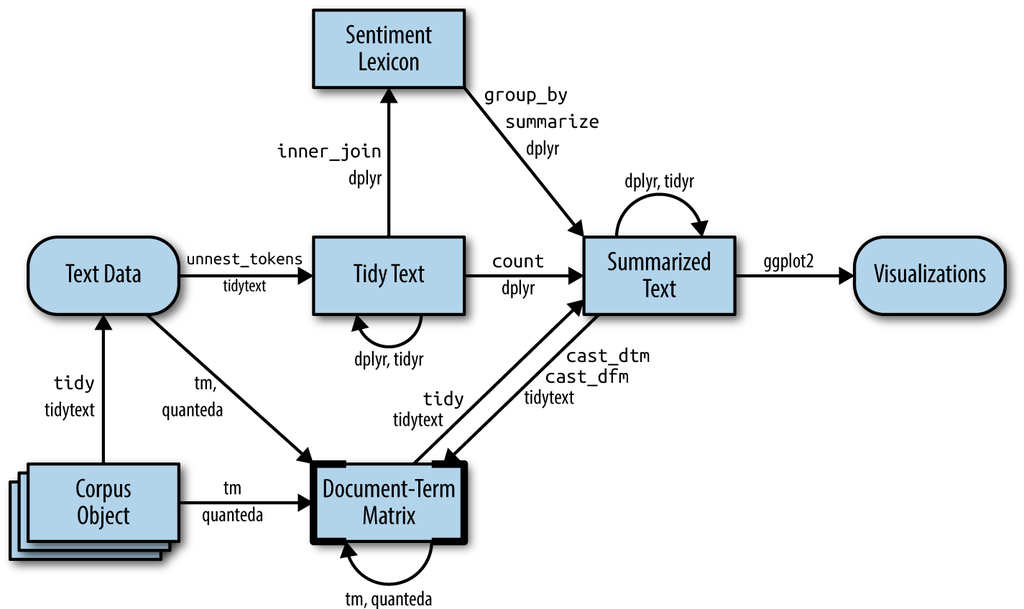
\includegraphics{/Users/chenjuqiang/Nutstore Files/310_Tutorial/Language data science/data/ch6/textConversion.png}
\caption{美丽的风景}
\end{figure}

任务1
导入白鲸的文本
自动提取文本中的章节信息,形成结构化的语料库。

\begin{Shaded}
\begin{Highlighting}[]
\CommentTok{# install.packages("quanteda")}
\CommentTok{# install.packages("devtools")}
\CommentTok{# }
\CommentTok{# devtools::install_github("quanteda/quanteda.corpora")}
\CommentTok{# devtools::install_github("kbenoit/quanteda.dictionaries")}
\KeywordTok{library}\NormalTok{(tidyverse)}
\KeywordTok{library}\NormalTok{(quanteda)}
\CommentTok{#install.packages("readtext")}
\KeywordTok{require}\NormalTok{(readtext)}

\CommentTok{#install.packages("tidytext")}
\KeywordTok{library}\NormalTok{(tidytext)}
\KeywordTok{library}\NormalTok{(tokenizers)}

\CommentTok{# text analysis data wrangling}
\CommentTok{# import from a text file}
\NormalTok{melville.v =}\StringTok{ }\KeywordTok{scan}\NormalTok{(}\StringTok{"data/ch6/melville.txt"}\NormalTok{, }
              \DataTypeTok{what =} \StringTok{"character"}\NormalTok{,}
              \DataTypeTok{sep =} \StringTok{"}\CharTok{\textbackslash{}n}\StringTok{"}\NormalTok{)}

\CommentTok{# convert the vector into a dataframe}
\NormalTok{melville.fullsent =}\StringTok{ }\KeywordTok{paste}\NormalTok{(melville.v, }\DataTypeTok{collapse =} \StringTok{"}\CharTok{\textbackslash{}n}\StringTok{"}\NormalTok{)}

\NormalTok{melville.fullsent <-}\StringTok{ }\KeywordTok{tokenize_sentences}\NormalTok{(melville.fullsent)}

\NormalTok{melville.fullsent.df =}\StringTok{ }\KeywordTok{data.frame}\NormalTok{(melville.fullsent )}

\KeywordTok{colnames}\NormalTok{(melville.fullsent.df ) =}\StringTok{ "text"}

\CommentTok{# import from a text file but seperate by period}
\NormalTok{melville.b =}\StringTok{ }\KeywordTok{scan}\NormalTok{(}\StringTok{"data/ch6/melville.txt"}\NormalTok{,}
              \DataTypeTok{what =} \StringTok{"character"}\NormalTok{,}
              \DataTypeTok{sep =} \StringTok{"."}\NormalTok{)}

\NormalTok{melville.df =}\StringTok{ }\KeywordTok{data.frame}\NormalTok{(melville.b)}\OperatorTok
\StringTok{  }\KeywordTok{mutate}\NormalTok{(}\DataTypeTok{linenumber =} \KeywordTok{row_number}\NormalTok{(),}
         \DataTypeTok{chapter =} \KeywordTok{cumsum}\NormalTok{(}\KeywordTok{str_detect}\NormalTok{(melville.b, }\KeywordTok{regex}\NormalTok{(}\StringTok{"^CHAPTER [}\CharTok{\textbackslash{}\textbackslash{}}\StringTok{divxlc]"}\NormalTok{))))}

\NormalTok{melville.df2 =}\StringTok{ }\NormalTok{melville.fullsent.df }\OperatorTok
\StringTok{    }\KeywordTok{mutate}\NormalTok{(}\DataTypeTok{linenumber =} \KeywordTok{row_number}\NormalTok{(),}
           \DataTypeTok{chapter =} \KeywordTok{cumsum}\NormalTok{(}\KeywordTok{str_detect}\NormalTok{(melville.fullsent.df, }\KeywordTok{regex}\NormalTok{(}\StringTok{"^CHAPTER [0-9]\{1,2\}"}\NormalTok{))))}



\CommentTok{# 数据导入}
\NormalTok{melville <-}\StringTok{ }\KeywordTok{scan}\NormalTok{(}\DataTypeTok{file=}\StringTok{"data/ch6/melville.txt"}\NormalTok{, }
             \DataTypeTok{what=}\StringTok{"character"}\NormalTok{, }
             \DataTypeTok{sep=}\StringTok{"}\CharTok{\textbackslash{}n}\StringTok{"}\NormalTok{)}

\NormalTok{corps.melville=}\StringTok{ }\KeywordTok{data.frame}\NormalTok{(melville)}\OperatorTok
\StringTok{  }\KeywordTok{mutate}\NormalTok{(}\DataTypeTok{linenumber =} \KeywordTok{row_number}\NormalTok{(),}
         \DataTypeTok{chapter =} \KeywordTok{cumsum}\NormalTok{(}\KeywordTok{str_detect}\NormalTok{(melville, }\KeywordTok{regex}\NormalTok{(}\StringTok{"^CHAPTER [1-9]\{1,2\}"}\NormalTok{))))}\OperatorTok
\StringTok{  }\KeywordTok{corpus}\NormalTok{(}\DataTypeTok{text_field =} \StringTok{"melville"}\NormalTok{)}

\NormalTok{corps.melville =}\StringTok{ }\KeywordTok{corpus}\NormalTok{(df.melville)}

\KeywordTok{summary}\NormalTok{(corps.melville, }\DecValTok{50}\NormalTok{)}

\NormalTok{corps.melville.body =}\StringTok{ }\KeywordTok{corpus_subset}\NormalTok{(corps.melville, }
\NormalTok{                                    chapter }\OperatorTok{>}\StringTok{ }\DecValTok{0}\NormalTok{)}

\KeywordTok{summary}\NormalTok{(corps.melville.body, }\DecValTok{50}\NormalTok{)}
\end{Highlighting}
\end{Shaded}

任务2
批量导入econmist文件

\begin{Shaded}
\begin{Highlighting}[]
\CommentTok{### 方法1}
\CommentTok{# 批量导入}
\NormalTok{filenames =}\StringTok{ }\KeywordTok{list.files}\NormalTok{(}\DataTypeTok{path =} \StringTok{"data/ch6/economist_20110101"}\NormalTok{, }\DataTypeTok{pattern =} \StringTok{".txt"}\NormalTok{, }\DataTypeTok{full.names =} \OtherTok{TRUE}\NormalTok{)}

\CommentTok{# wd = getwd()}
\CommentTok{# bin = scan(file=paste(wd,filename[2], sep = "/"), what="character", sep="\textbackslash{}n")}
\NormalTok{binv =}\StringTok{ }\KeywordTok{vector}\NormalTok{()}
\NormalTok{bin =}\StringTok{ }\KeywordTok{tibble}\NormalTok{()}
\NormalTok{df.eco =}\StringTok{ }\KeywordTok{tibble}\NormalTok{()}
\ControlFlowTok{for}\NormalTok{ (i }\ControlFlowTok{in} \DecValTok{1}\OperatorTok{:}\KeywordTok{length}\NormalTok{(filenames)) \{}
  \CommentTok{#}
\NormalTok{  binv =}\StringTok{ }\KeywordTok{scan}\NormalTok{(}\DataTypeTok{file=}\NormalTok{ filenames[i], }
              \DataTypeTok{what=}\StringTok{"character"}\NormalTok{, }
              \DataTypeTok{sep=}\StringTok{"}\CharTok{\textbackslash{}n}\StringTok{"}\NormalTok{)}
  \CommentTok{#}
\NormalTok{  bin =}\StringTok{ }\KeywordTok{tibble}\NormalTok{(}\DataTypeTok{article =} \KeywordTok{str_extract}\NormalTok{(filenames[i], }
                                     \DataTypeTok{pattern =} \StringTok{"/[0-9]\{2\}"}\NormalTok{),}
                                     \DataTypeTok{text =}\NormalTok{ binv)}
\NormalTok{ df.eco  =}\StringTok{ }\KeywordTok{rbind}\NormalTok{(bin,df.eco )}
\NormalTok{\}}

\KeywordTok{head}\NormalTok{( df.eco)}

\CommentTok{### 方法2}
\CommentTok{# 多文本文件}
\NormalTok{df.economist <-}\StringTok{ }\KeywordTok{readtext}\NormalTok{(}\StringTok{"data/ch6/economist_20110101/*txt"}\NormalTok{, }
                    \DataTypeTok{cache =} \OtherTok{FALSE}\NormalTok{)}
\NormalTok{corps.economist =}\StringTok{ }\KeywordTok{corpus}\NormalTok{(df.economist)}
\KeywordTok{summary}\NormalTok{(}\KeywordTok{corpus}\NormalTok{(corps.economist), }\DecValTok{5}\NormalTok{)}
\end{Highlighting}
\end{Shaded}

任务3
数据整理莎士比亚十四行诗

\begin{Shaded}
\begin{Highlighting}[]
\CommentTok{# 批量导入}

\NormalTok{filenames =}\StringTok{ }\KeywordTok{list.files}\NormalTok{(}\DataTypeTok{path =} \StringTok{"data/ch6/sonnet"}\NormalTok{, }\DataTypeTok{pattern =} \StringTok{".txt"}\NormalTok{, }\DataTypeTok{full.names =} \OtherTok{TRUE}\NormalTok{)}

\NormalTok{binv =}\StringTok{ }\KeywordTok{vector}\NormalTok{()}
\NormalTok{bin =}\StringTok{ }\KeywordTok{tibble}\NormalTok{()}
\NormalTok{df.sonnet =}\StringTok{ }\KeywordTok{tibble}\NormalTok{()}
\ControlFlowTok{for}\NormalTok{ (i }\ControlFlowTok{in} \DecValTok{1}\OperatorTok{:}\KeywordTok{length}\NormalTok{(filenames)) \{}
\NormalTok{  binv =}\StringTok{ }\KeywordTok{scan}\NormalTok{(}\DataTypeTok{file=}\NormalTok{ filenames[i], }\DataTypeTok{what=}\StringTok{"character"}\NormalTok{, }\DataTypeTok{sep=}\StringTok{"}\CharTok{\textbackslash{}n}\StringTok{"}\NormalTok{)}
\NormalTok{  bin =}\StringTok{ }\KeywordTok{tibble}\NormalTok{(}\DataTypeTok{article =} \KeywordTok{str_extract}\NormalTok{(filenames[i], }\DataTypeTok{pattern =} \StringTok{"sonnet_[0-9]\{1,3\}"}\NormalTok{),}
               \DataTypeTok{text =}\NormalTok{ binv)}
\NormalTok{  df.sonnet =}\StringTok{ }\KeywordTok{rbind}\NormalTok{(bin,df.sonnet)}
\NormalTok{\}}

\KeywordTok{head}\NormalTok{(df.sonnet)}


\NormalTok{sonnet_clean1 =}\StringTok{ }\NormalTok{df.sonnet }\OperatorTok
\StringTok{  }\CommentTok{# 分词}
\StringTok{  }\KeywordTok{unnest_tokens}\NormalTok{(word, text)}\OperatorTok
\StringTok{  }\CommentTok{# remove stop words}
\StringTok{  }\KeywordTok{anti_join}\NormalTok{(}\KeywordTok{get_stopwords}\NormalTok{())}


\CommentTok{# 方法2}
\CommentTok{# 包含取自文件名的docvars的多个文本文件}
\NormalTok{df.sonnet <-}\StringTok{ }\KeywordTok{readtext}\NormalTok{(}\StringTok{"data/ch6/sonnet/*txt"}\NormalTok{,}
                             \DataTypeTok{docvarsfrom =} \StringTok{"filenames"}\NormalTok{, }
                             \DataTypeTok{dvsep =} \StringTok{"_"}\NormalTok{, }
                       \DataTypeTok{docvarnames =} \KeywordTok{c}\NormalTok{(}\StringTok{"author"}\NormalTok{,}\StringTok{"article"}\NormalTok{, }\StringTok{"title"}\NormalTok{))}

\NormalTok{corps.sonnet =}\StringTok{ }\KeywordTok{corpus}\NormalTok{(df.sonnet)}
\KeywordTok{summary}\NormalTok{(}\KeywordTok{corpus}\NormalTok{(df.sonnet), }\DecValTok{5}\NormalTok{)}
\end{Highlighting}
\end{Shaded}

任务4
导入BNC的xml文件

xml

\begin{Shaded}
\begin{Highlighting}[]
\CommentTok{# library(XML)}
\CommentTok{# library(methods)}
\CommentTok{# }
\CommentTok{# # install.packages("xml2")}
\CommentTok{# library(xml2)}
\CommentTok{# a = read_xml("data/ch6/BNC_BABY/2553.xml")}
\CommentTok{# c = xml_text(a)}
\CommentTok{# result <- xmlParse(file = "data/ch6/BNC_BABY/2553.xml")}
\CommentTok{# }
\CommentTok{# result <- xmlParse(file = "data/ch6/BNC_BABY/download/Texts/aca/A6U.xml")}
\CommentTok{# h %>%}
\CommentTok{#   unnest_tokens(word, text, format = "html")}
\CommentTok{# text.v = scan("data/ch6/BNC_BABY/2553.xml", }
\CommentTok{#               what = "character",}
\CommentTok{#               sep = "\textbackslash{}n")}
\CommentTok{# }
\CommentTok{# rootnode <- xmlRoot(result)}
\CommentTok{# }
\CommentTok{# xmldataframe <- xmlToDataFrame("data/ch6/BNC_BABY/2553.xml")}
\CommentTok{# }
\CommentTok{# xmldataframe <- xmlToDataFrame("data/ch6/BNC_BABY/download/Texts/aca/A6U.xml")}
\CommentTok{# read_xml("data/ch6/BNC_BABY/download/Texts/aca/A6U.xml")%>%}
\CommentTok{#   xml_text()}
\CommentTok{# }
\CommentTok{# }
\CommentTok{# xml_ns(a)}
\end{Highlighting}
\end{Shaded}

任务 5 在线导入

\begin{Shaded}
\begin{Highlighting}[]
\CommentTok{# library(gutenbergr)}
\CommentTok{# }
\CommentTok{# gutenberg_metadata = data.frame(gutenberg_metadata)}


\CommentTok{#总数}

\CommentTok{#作者及著作数}

\CommentTok{#主题分类}

\CommentTok{#查找谋一本书}
\CommentTok{# gutenberg_metadata %>%}
\CommentTok{#   filter(title == "Wuthering Heights")}
\CommentTok{# }
\CommentTok{# #找某一个作者}
\CommentTok{# gutenberg_metadata %>%}
\CommentTok{#   filter(author == "James, William")}
\CommentTok{# }
\CommentTok{# #主题查找}
\CommentTok{# gutenberg_subjects %>%}
\CommentTok{#   filter(subject == "Detective and mystery stories")}



\CommentTok{#作家信息}
\CommentTok{# gutenberg_authors%>%}
\CommentTok{#     filter(author == "Detective and mystery stories")}
\CommentTok{# }
\CommentTok{# # }
\CommentTok{# }
\CommentTok{# books <- gutenberg_download(c(621,5116), meta_fields = "title")}
\CommentTok{# }
\CommentTok{# william.james = books}
\CommentTok{# write.csv(william.james, file = "william.james.csv", row.names = FALSE)}
\CommentTok{# }
\CommentTok{# physics <- gutenberg_download(c(37729, 14725, 13476, 30155), }
\CommentTok{#                               meta_fields = "author")}
\CommentTok{# }
\CommentTok{# physics.word = physics%>%}
\CommentTok{#   unnest_tokens(word, text) %>%}
\CommentTok{#   count(author, word, sort = TRUE)}
\CommentTok{# }
\CommentTok{# write.csv(physics, file = "physics.csv", row.names = FALSE)}
\end{Highlighting}
\end{Shaded}

\hypertarget{concordance}{%
\subsection{concordance}\label{concordance}}

在语料库语言学中,concordance(词汇共现)是指查找和展示给定词汇或短语在语料库中的上下文环境,以便深入理解该词汇或短语的用法和含义。通常,concordance结果以关键词出现的句子或文本段落的片段形式呈现,同时显示关键词前后的上下文内容。

任务
请使用kwic()完成一下任务
《白鲸》中whale出现的语境
莎士比亚十四行诗中love出现的语境。
economist中China出现的语境。

\begin{Shaded}
\begin{Highlighting}[]
\CommentTok{# 测试一下是否需要tokenisation}
\NormalTok{corps.melville.body }
\KeywordTok{kwic}\NormalTok{(corps.melville.body, }\DataTypeTok{pattern =} \StringTok{"whale"}\NormalTok{, }\DataTypeTok{valuetype =} \StringTok{"fixed"}\NormalTok{, }\DataTypeTok{window =} \DecValTok{3}\NormalTok{)}

\NormalTok{corps.sonnet }

\KeywordTok{kwic}\NormalTok{(corps.sonnet , }\DataTypeTok{pattern =} \StringTok{"love"}\NormalTok{, }\DataTypeTok{valuetype =} \StringTok{"regex"}\NormalTok{, }\DataTypeTok{window =} \DecValTok{3}\NormalTok{)}


\NormalTok{corps.economist}

\NormalTok{kwic.data =}\StringTok{ }\KeywordTok{kwic}\NormalTok{(corps.economist, }\DataTypeTok{pattern =} \StringTok{"China"}\NormalTok{, }\DataTypeTok{valuetype =} \StringTok{"fixed"}\NormalTok{, }\DataTypeTok{window =} \DecValTok{3}\NormalTok{)}

\KeywordTok{as.as.data.frame}\NormalTok{(kwic.data)}

\KeywordTok{kwic}\NormalTok{(corps.economist, }\DataTypeTok{pattern =} \KeywordTok{phrase}\NormalTok{(}\StringTok{"United States"}\NormalTok{)) }\OperatorTok{|}\ErrorTok{>}
\StringTok{    }\KeywordTok{head}\NormalTok{()}
\end{Highlighting}
\end{Shaded}

英语的自然语言预处理通常包含以下步骤:

\begin{enumerate}
\def\labelenumi{\arabic{enumi}.}
\item
  分词(Tokenization):将连续的文本切分成独立的词汇单位(token)。这是NLP处理的第一步,为后续的文本分析打下基础。
\item
  去除停用词(Stopwords Removal):去除常见的无实际意义的词汇,如``the''、``and''、``in''等。这些词汇通常不对文本分析产生实质性的影响。
\item
  文本转换为小写(Lowercasing):将所有文本转换为小写形式。这样可以统一不同大小写形式的单词,避免出现重复计数。
\item
  去除标点符号(Punctuation Removal):去除文本中的标点符号,如逗号、句号、问号等。这些符号通常对文本分析没有实际帮助。
\item
  词干提取(Stemming)或词形还原(Lemmatization):对单词进行规范化处理,将其转换为词根形式或原始形式。这有助于减少不同词形造成的单词多样性。
\item
  去除特殊字符(Special Characters Removal):去除文本中的特殊字符,如HTML标签、网址、邮箱地址等。
\item
  数字处理:根据需求,可以将数字转换为特定标记,保留数字等。
\item
  词袋模型(Bag-of-Words)或词向量表示:将文本转换成数值形式,以便于计算机处理和分析。词袋模型将文本表示为词汇的频次向量,而词向量表示则将词汇映射为实数向量,以捕捉词汇之间的语义关系。
\end{enumerate}

这些预处理步骤是在进行文本分析、情感分析、主题建模、文本分类等任务前常见的基础操作,能够帮助提高文本分析的效率和准确性。预处理过程中的具体步骤和顺序可以根据不同的任务和需求进行调整和定制。

\hypertarget{ux6587ux672cux9884ux5904ux7406}{%
\subsection{文本预处理}\label{ux6587ux672cux9884ux5904ux7406}}

\begin{Shaded}
\begin{Highlighting}[]
\CommentTok{# 示例数据集:学生英语写作}
\NormalTok{student_writings <-}\StringTok{ }\KeywordTok{data.frame}\NormalTok{(}
  \DataTypeTok{id =} \KeywordTok{c}\NormalTok{(}\DecValTok{1}\NormalTok{, }\DecValTok{2}\NormalTok{, }\DecValTok{3}\NormalTok{),}
  \DataTypeTok{text =} \KeywordTok{c}\NormalTok{(}\StringTok{"My favorite hobby is playing basketball. It is a fun and challenging sport."}\NormalTok{,}
           \StringTok{"In my opinion, reading books is a great way to learn new things and expand my knowledge."}\NormalTok{,}
           \StringTok{"I love traveling and exploring new places. It allows me to experience different cultures and traditions."}\NormalTok{)}
\NormalTok{)}

\CommentTok{# 查看数据集}
\KeywordTok{print}\NormalTok{(student_writings)}

\CommentTok{# 使用quanteda的tokenize函数进行分词}
\NormalTok{tokens <-}\StringTok{ }\KeywordTok{tokenize}\NormalTok{(student_writings}\OperatorTok{$}\NormalTok{text, }
                    \DataTypeTok{remove_punct =} \OtherTok{TRUE}\NormalTok{, }
                    \DataTypeTok{remove_numbers =}\NormalTok{ TRUE,}
                    \DataTypeTok{remove_separators =} \OtherTok{FALSE}\NormalTok{)}


\NormalTok{tokens <-}\StringTok{ }\KeywordTok{tokenize}\NormalTok{(student_writings}\OperatorTok{$}\NormalTok{text, }
                    \DataTypeTok{what =} \StringTok{"character"}
                    \DataTypeTok{remove_punct =} \OtherTok{TRUE}\NormalTok{, }
                    \DataTypeTok{remove_numbers =}\NormalTok{ TRUE,}
                    \DataTypeTok{remove_separators =} \OtherTok{FALSE}\NormalTok{)}
\NormalTok{tokens <-}\StringTok{ }\KeywordTok{tokenize}\NormalTok{(student_writings}\OperatorTok{$}\NormalTok{text, }
                    \DataTypeTok{what =} \StringTok{"sentencce"}
                    \DataTypeTok{remove_punct =} \OtherTok{TRUE}\NormalTok{, }
                    \DataTypeTok{remove_numbers =}\NormalTok{ TRUE,}
                    \DataTypeTok{remove_separators =} \OtherTok{FALSE}\NormalTok{)}

\NormalTok{tokens <-}\StringTok{ }\KeywordTok{tokenize}\NormalTok{(student_writings}\OperatorTok{$}\NormalTok{text, }
                    \DataTypeTok{what =} \StringTok{"sentencce"}
                    \DataTypeTok{remove_punct =} \OtherTok{TRUE}\NormalTok{, }
                    \DataTypeTok{remove_numbers =}\NormalTok{ TRUE,}
                    \DataTypeTok{remove_separators =} \OtherTok{FALSE}\NormalTok{)}\OperatorTok
\StringTok{          }\KeywordTok{tokens_remove}\NormalTok{(}\KeywordTok{stopwords}\NormalTok{(}\StringTok{"en"}\NormalTok{))}
\KeywordTok{tokens}\NormalTok{(}\StringTok{"New York City is located in the United States."}\NormalTok{) }\OperatorTok{|}\ErrorTok{>}
\StringTok{    }\KeywordTok{tokens_compound}\NormalTok{(}\DataTypeTok{pattern =} \KeywordTok{phrase}\NormalTok{(}\KeywordTok{c}\NormalTok{(}\StringTok{"New York City"}\NormalTok{, }\StringTok{"United States"}\NormalTok{)))}\OperatorTok
\StringTok{    }\KeywordTok{tokens_wordstem}\NormalTok{(}\DataTypeTok{language =} \StringTok{"en"}\NormalTok{)}

\KeywordTok{tokens}\NormalTok{(}\StringTok{"one~two~three"}\NormalTok{) }\OperatorTok{|}\ErrorTok{>}
\StringTok{    }\KeywordTok{tokens_split}\NormalTok{(}\DataTypeTok{separator =} \StringTok{"~"}\NormalTok{)}
\end{Highlighting}
\end{Shaded}

为了简单地对文本进行分词,quanteda提供了一个强大的命令称为tokens()。这将生成一个中间对象,由字符向量形式的令牌列表组成,列表中的每个元素对应于输入文档。

使用tidytext

\begin{Shaded}
\begin{Highlighting}[]
\CommentTok{# 以句子为单位}
\NormalTok{tidy.eco.sent =}\StringTok{ }\NormalTok{df.economist }\OperatorTok
\StringTok{  }\CommentTok{# 分词}
\StringTok{  }\KeywordTok{unnest_tokens}\NormalTok{(sentence, text, }\DataTypeTok{token =} \StringTok{"sentences"}\NormalTok{)}\OperatorTok
\StringTok{  }\KeywordTok{mutate}\NormalTok{(}\DataTypeTok{sentence_id =} \DecValTok{1}\OperatorTok{:}\KeywordTok{n}\NormalTok{())}\OperatorTok
\StringTok{  }\KeywordTok{unnest_tokens}\NormalTok{(word, sentence)}\OperatorTok
\StringTok{  }\CommentTok{# 去除无实意词}
\StringTok{  }\KeywordTok{anti_join}\NormalTok{(}\KeywordTok{get_stopwords}\NormalTok{())}

\CommentTok{# 以文章为单位}
\NormalTok{data_clean1 =}\StringTok{  }\NormalTok{df.eco }\OperatorTok
\StringTok{  }\CommentTok{# 分词}
\StringTok{  }\KeywordTok{unnest_tokens}\NormalTok{(word, text)}\OperatorTok
\StringTok{  }\CommentTok{# remove stop words}
\StringTok{  }\KeywordTok{anti_join}\NormalTok{(}\KeywordTok{get_stopwords}\NormalTok{())}

\CommentTok{# 以句子为单位}
\NormalTok{data_clean2 =}\StringTok{  }\NormalTok{df.eco }\OperatorTok
\StringTok{  }\CommentTok{# 分词}
\StringTok{  }\KeywordTok{unnest_tokens}\NormalTok{(sentence, text, }\DataTypeTok{token =} \StringTok{"sentences"}\NormalTok{)}\OperatorTok
\StringTok{  }\KeywordTok{mutate}\NormalTok{(}\DataTypeTok{sentence_id =} \DecValTok{1}\OperatorTok{:}\KeywordTok{n}\NormalTok{())}\OperatorTok
\StringTok{  }\KeywordTok{unnest_tokens}\NormalTok{(word, sentence)}\OperatorTok
\StringTok{  }\CommentTok{# 去除无实意词}
\StringTok{  }\KeywordTok{anti_join}\NormalTok{(}\KeywordTok{get_stopwords}\NormalTok{())}

\CommentTok{# 以诗为单位}
\NormalTok{tidy.sonnet =}\StringTok{ }\NormalTok{df.sonnet }\OperatorTok
\StringTok{  }\CommentTok{# 分词}
\StringTok{  }\KeywordTok{unnest_tokens}\NormalTok{(word, text)}\OperatorTok
\StringTok{  }\CommentTok{# remove stop words}
\StringTok{  }\KeywordTok{anti_join}\NormalTok{(}\KeywordTok{get_stopwords}\NormalTok{())}

\NormalTok{tidy.sonnet.freq =}\StringTok{ }\NormalTok{tidy.sonnet }\OperatorTok
\StringTok{  }\KeywordTok{group_by}\NormalTok{(title,word)}\OperatorTok
\StringTok{  }\KeywordTok{count}\NormalTok{()}\OperatorTok
\StringTok{  }\KeywordTok{group_by}\NormalTok{(title)}\OperatorTok
\StringTok{  }\KeywordTok{mutate}\NormalTok{(}\DataTypeTok{total =} \KeywordTok{sum}\NormalTok{(n),}
         \DataTypeTok{proportion =}\NormalTok{ n}\OperatorTok{/}\NormalTok{total)}
\end{Highlighting}
\end{Shaded}

\hypertarget{ux6784ux5efaux6587ux6863ux7279ux5f81ux77e9ux9635}{%
\section{构建文档特征矩阵}\label{ux6784ux5efaux6587ux6863ux7279ux5f81ux77e9ux9635}}

为了进行统计分析,例如文档缩放(document scaling),我们需要提取一个矩阵,将某些特征的值与每个文档关联起来。在quanteda中,我们使用dfm()函数来生成这样的矩阵。``dfm''是文档特征矩阵(document-feature matrix)的缩写,它总是将文档放在行上,将``特征''放在列上。我们固定了这种维度方向,因为在数据分析中,将分析单元作为行,将与每个单元相关的特征或变量作为列是标准做法。我们称其为``特征''而不是``词汇''(terms),因为特征比词汇更加通用:它们可以被定义为原始词汇、词干化后的词汇、词汇的词性、去除停用词后的词汇,或者属于某个词汇所属的字典类别。特征可以非常通用,例如ngrams或句法依赖关系,我们将其保持开放式。

\hypertarget{ux4e2dux6587ux81eaux7136ux8bedux8a00ux9884ux5904ux7406}{%
\subsection{中文自然语言预处理}\label{ux4e2dux6587ux81eaux7136ux8bedux8a00ux9884ux5904ux7406}}

\begin{Shaded}
\begin{Highlighting}[]
\CommentTok{# 创建英国留学生的中文作文数据集}
\NormalTok{chinese_essays <-}\StringTok{ }\KeywordTok{c}\NormalTok{(}
  \StringTok{"我是一名来自英国的留学生。我喜欢学习中文,因为中文是一门非常有趣的语言。"}\NormalTok{,}
  \StringTok{"在英国,我学习了中文两年。现在我已经可以用中文进行简单的对话了。"}\NormalTok{,}
  \StringTok{"我喜欢中国的文化和风景。我希望能在中国留学更长的时间。"}
\NormalTok{)}
\end{Highlighting}
\end{Shaded}

\hypertarget{ux7b2cux516bux7ae0-ux8bedux97f3ux5e93ux6784ux5efa}{%
\chapter{第八章 语音库构建}\label{ux7b2cux516bux7ae0-ux8bedux97f3ux5e93ux6784ux5efa}}

We have finished a nice book.

\hypertarget{ux7b2cux4e5dux7ae0-ux6570ux636eux7edfux8ba1ux5efaux6a21ux57faux7840}{%
\chapter{第九章 数据统计建模基础}\label{ux7b2cux4e5dux7ae0-ux6570ux636eux7edfux8ba1ux5efaux6a21ux57faux7840}}

\hypertarget{ux4eceux6570ux636eux53efux89c6ux5316ux5230ux7edfux8ba1ux5efaux6a21}{%
\section{从数据可视化到统计建模}\label{ux4eceux6570ux636eux53efux89c6ux5316ux5230ux7edfux8ba1ux5efaux6a21}}

数据中的模式提供了关于关系或协变性的线索。现在我们知道如何可视化不同的关系,我们可以继续学习如何对这些关系进行形式化测试。

统计模型是从数据中提取模式的工具。

统计学代表了一种常见的方法,用于展示信息,帮助我们理解数据所传达的信息。

描述性(或总结性)统计学总结原始数据,使数据用户更容易解释数据集。描述性统计学可以描述数据集的形状、中心和散布。

推断统计学用于从样本推断出关于总体的结论。它包括估计(估计是根据从总体的样本收集的数据推断出来的值),以及假设检验。

\hypertarget{ux4e24ux4e2aux8fdeux7eedux53d8ux91cf-1}{%
\subsection{两个连续变量}\label{ux4e24ux4e2aux8fdeux7eedux53d8ux91cf-1}}

\hypertarget{ux7b80ux5355ux7ebfux6027ux56deux5f52}{%
\subsubsection{简单线性回归}\label{ux7b80ux5355ux7ebfux6027ux56deux5f52}}

在这里使用的技术称为简单线性回归,其中有一个因变量(连续)和一个自变量(连续)。当有多个自变量(连续)时,需要寻找称为多元线性回归的方法。

\hypertarget{ux76f8ux5173ux6027-vs.ux7ebfux6027ux56deux5f52}{%
\paragraph{相关性 vs.~线性回归}\label{ux76f8ux5173ux6027-vs.ux7ebfux6027ux56deux5f52}}

相关性和线性回归都探讨了两个定量变量之间的关系。(Salvatore S. Mangiafico)

相关性确定了一个变量是否随着另一个变量的变化而有系统地变化。它不指定哪个变量是因变量,哪个是自变量。通常,查看数据集中哪些变量与其他变量相关是很有用的,尤其是看哪些变量与特定感兴趣的变量相关。

相比之下,线性回归指定一个变量为自变量,另一个为因变量。由此产生的模型将这两个变量之间的关系表示为线性关系。

与线性回归相关的测试是参数化的,并假设残差服从正态分布、方差齐性、残差独立性以及两个变量之间的线性关系。

\hypertarget{correlation-matrix}{%
\paragraph{Correlation matrix}\label{correlation-matrix}}

效应大小

统计学中的r、rho和tau分别用作Pearson、Spearman和Kendall回归的效应大小指标。这些统计量的取值范围是-1到1,其中0表示没有相关性,1表示完美的正相关,-1表示完美的负相关。与其他效应大小统计量一样,这些统计量不受样本大小的影响。

效应大小的解释因学科和实验预期而异,不应被视为普遍适用的。Cohen(1988)提供了关于r的解释。类似的解释可能适用于rho和tau。

小效应:0.10 - \textless{} 0.30

中等效应:0.30 - \textless{} 0.50

大效应:≥ 0.50

\hypertarget{pearsonux76f8ux5173ux6027}{%
\paragraph{Pearson相关性}\label{pearsonux76f8ux5173ux6027}}

Pearson相关性测试是一种参数化分析,要求变量之间的关系是线性的,并且数据是双变量正态分布的。变量应为区间/比率变量。该测试对异常值敏感。

相关系数r的取值范围是+1到-1,+1表示完美的正相关,-1表示完美的负相关。r=0表示没有任何相关性。假设检验确定r值是否与0显著不同。

\hypertarget{kendallux76f8ux5173ux6027}{%
\paragraph{Kendall相关性}\label{kendallux76f8ux5173ux6027}}

Kendall相关性被视为一种非参数分析方法:
- 它是一种基于排名的测试,不需要对数据的分布做出假设。
- 变量可以是区间/比率变量或序数变量。

该测试的相关系数是tau,它的取值范围是+1到-1,其中+1表示完美的正相关,-1表示完美的负相关。tau=0表示没有任何相关性。假设检验确定tau值是否与0显著不同。

作为技术说明,在R中的cor.test函数计算的是tau-b,它能很好地处理排名中的并列情况。

该测试对数据中的异常值相对稳健。该测试有时被认为在样本数量较少或排名中存在许多并列情况时是可靠的。

\hypertarget{spearmanux76f8ux5173ux6027}{%
\paragraph{Spearman相关性}\label{spearmanux76f8ux5173ux6027}}

Spearman相关性被视为一种非参数分析方法:

它是一种基于排名的测试,不需要对数据的分布做出假设。
变量可以是区间/比率变量或序数变量。
该测试的相关系数是rho,它的取值范围是+1到-1,其中+1表示完美的正相关,-1表示完美的负相关。rho=0表示没有任何相关性。假设检验确定rho值是否与0显著不同。

Spearman相关性在使用序数数据时可能最常用。它检验变量之间是否存在单调关系。该测试对数据中的异常值相对稳健。

\hypertarget{ux7ebfux6027ux56deux5f52}{%
\paragraph{线性回归}\label{ux7ebfux6027ux56deux5f52}}

线性回归是一种非常常见的方法,用于建模两个区间/比率变量之间的关系。线性回归的结果包括估计线性模型的截距和斜率。

多个自变量、名义变量和序数变量

如果模型中有多个区间/比率类型的自变量,则线性回归会扩展为多元回归。

如果自变量是名义类型的,则线性回归将变为单因素方差分析。

处理序数类型的自变量可能会更加复杂。通常,它们被视为名义类型或区间/比率类型,但每种方法都有缺点。

假设

线性回归假设:
- 两个变量之间存在线性关系,
- 残差服从正态分布,
- 残差是独立的,
- 残差的方差是齐次的。

可以使用lm函数执行线性回归,该函数与我们用于方差分析的函数相同。

如何解读线性回归模型?

该模型给出了截距(-1.87)和斜率(0.07)的系数;

每个系数都有三个其他数字:标准误差、t值和p值。P值告诉我们系数是否与零显著不同。

如果一个预测变量的系数为零,则该预测变量与因变量之间没有任何关系,因此它作为预测变量毫无用处。为了确定系数是否与零显著不同,从而有可能有用,会进行双尾t检验,使用t值和相关的自由度。

t值本身是系数除以其标准误差得到的值。标准误差是系数估计的可信程度的一种度量。标准误差越小,估计的系数周围的置信区间越小,零包含在接受区域的可能性就越小,因此该系数可能为零的概率也越小。

残差标准误差是衡量模型不成功的一个指标;它衡量了因变量中我们通过预测变量无法解释的变异性。模型越好,其残差标准误差就越小。

多重R方为0.8115。这个R方是平方相关系数r²,用于从0到1的范围内量化模型解释的方差的比例。

\hypertarget{ux5206ux7c7bux81eaux53d8ux91cfux548cux8fdeux7eedux56e0ux53d8ux91cfux53d8ux91cf}{%
\subsection{分类(自变量)和连续(因变量)变量}\label{ux5206ux7c7bux81eaux53d8ux91cfux548cux8fdeux7eedux56e0ux53d8ux91cfux53d8ux91cf}}

\hypertarget{tux68c0ux9a8c}{%
\subsubsection{T检验}\label{tux68c0ux9a8c}}

T检验常用于比较两个样本的均值,或者将一个样本与固定值进行比较。换句话说,自变量应该是分类变量,并且具有两个水平。

要求:
组间的观测值是独立的。即非配对或重复测量数据。

每个总体的数据是正态分布的。如果数据分布是单峰且没有离群值,适度的偏斜是可以接受的。

\hypertarget{anovaux65b9ux5deeux5206ux6790}{%
\subsubsection{ANOVA(方差分析)}\label{anovaux65b9ux5deeux5206ux6790}}

当自变量有超过两个水平时,我们需要使用ANOVA进行分析。

我们可以在R中使用avo函数或构建线性模型进行ANOVA分析。
报告结果:在他们的中文成绩方面,不同班级之间存在显著差异,F(3, 96)= 0.87,p = 0.46。

在运行了模型之后,很可能需要进行两两比较。然而,我们不能简单地使用多个t检验,而是需要对alpha值进行修正。

有不同的修正方式:

\begin{enumerate}
\def\labelenumi{\arabic{enumi}.}
\tightlist
\item
  Bonferroni校正:a/n
\item
  Tukey的事实上显著差异(Honestly Significant Difference, HSD):假设每个因子水平的均值应该基于相同数量的观测。
\end{enumerate}

\hypertarget{ux4e24ux4e2aux5206ux7c7bux53d8ux91cf-1}{%
\subsection{两个分类变量}\label{ux4e24ux4e2aux5206ux7c7bux53d8ux91cf-1}}

\hypertarget{ux5361ux65b9ux68c0ux9a8c}{%
\subsubsection{卡方检验}\label{ux5361ux65b9ux68c0ux9a8c}}

当我们的数据涉及两个分类变量,并且我们想知道这两个变量是否相关或独立时,我们可以使用卡方检验。

独立性假设的零假设将被拒绝,如果以下卡方检验统计量的p值小于给定的显著性水平α。

以下是一个示例:在数据集survey中,Smoke列记录了学生的吸烟习惯,而Exer列记录了他们的锻炼水平。Smoke中允许的值为``Heavy''(频繁)、``Regul''(定期)、``Occas''(偶尔)和``Never''(从不)。至于Exer,它们是``Freq''(经常)、``Some''和``None''。

\hypertarget{ux53c2ux6570ux68c0ux9a8cux53caux76f8ux5173ux5047ux8bbe}{%
\section{参数检验及相关假设}\label{ux53c2ux6570ux68c0ux9a8cux53caux76f8ux5173ux5047ux8bbe}}

本部分进一步阐述了参数检验的假设以及评估这些假设的方法。

\hypertarget{ux53c2ux6570ux7edfux8ba1ux68c0ux9a8c}{%
\subsection{参数统计检验}\label{ux53c2ux6570ux7edfux8ba1ux68c0ux9a8c}}

T检验、方差分析和线性回归都是参数统计检验。它们用于依赖变量是区间/比率数据变量(如长度、高度、重量)的情况。

优点:

您的受众很可能熟悉这些技术和结果解释。

这些检验通常比非参数统计学检验更灵活、更强大。

缺点:

所有参数检验都假设关于底层数据分布的某种条件。如果这些假设不成立,产生的检验统计量将无效,而且测试的能力也不如满足假设的情况下那样强大。

计数/分类数据可能不适用于常见的参数检验。

\hypertarget{ux5047ux8bbe}{%
\subsection{假设}\label{ux5047ux8bbe}}

\begin{itemize}
\item
  随机抽样
  样本中捕获的数据是从整体人群中随机选择的。选择偏差显然会影响分析结果的有效性。
\item
  独立观测
  测试还将假设观测之间相互独立,除非分析考虑了非独立性。
\end{itemize}

例如,在重复测量实验中,同一主体随时间观察。测试日期较高的学生在后续日期上也有较高的测试分数。在这种情况下,一个日期上的观察不会独立于其他日期上的观察。独立性观察通常是从良好的实验设计中假设出来的。此外,数据或残差可以绘制,例如查看一个日期的观察是否与另一个日期的观察相关。

\begin{itemize}
\tightlist
\item
  数据或残差的正态分布
  参数检验假设数据来自已知分布的总体,例如正态分布。也就是说,一旦考虑了模型中变量的影响,数据应该是正态分布的。
\end{itemize}

实际上,这意味着分析的残差应该是正态分布的。这通常通过残差的直方图、密度图或分位数-分位数图进行评估。

有少数检验(限于单样本t检验、双样本t检验和配对t检验)要求数据本身是正态分布的。对于其他测试,将调查残差的分布。

残差,也常称为误差,是观察值与模型预测值之间的差异。例如,如果样本的计算均值为10,而一个观察值是12,那么该观察值的残差为2。请注意不要对此假设感到困惑。您可能会看到关于``数据''应该对参数检验进行正态分布的讨论。这通常是错误的。t检验假设每组的观测值是正态分布的,但是如果组之间有差异,我们可能会期望组合数据的是双峰分布,而不是简单的正态分布。这就是为什么在大多数情况下,我们关注残差的分布,而不是原始数据。

\begin{itemize}
\item
  方差的齐性
  参数分析还将假设各组方差齐性。也就是说,对于比较两组的学生t检验,每组的方差应该相同。方差的齐性也称为同方差性。
\item
  处理效应的可加性
  两因素方差分析模型和类似分析的模型构建为线性模型,其中依赖变量被预测为独立变量的线性组合。
\end{itemize}

对该假设的违反有时可以通过绘制残差与预测值的关系图来显示。

\hypertarget{ux5f02ux5e38ux503c}{%
\subsection{异常值}\label{ux5f02ux5e38ux503c}}

异常值是值远远超出预期范围的观察值。它们可能会对参数分析产生严重影响,因为它们影响了数据的分布并且强烈影响了均值。

有各种正式测试可以检测异常值,但它们不会在此进行讨论。最好的方法是在分析后查看残差。``残差与杠杆的关系''图和其他在下面``其他诊断图''部分的图形工具是好的工具。

某些参数检验对某些假设的违反具有一定的鲁棒性。例如,对于对称分布的正态性违反,t检验对其具有相当好的鲁棒性,但对样本方差不等(除非使用韦尔奇t检验)则没有。单因素方差分析对正态性的违反也有相当好的鲁棒性。

\ldots{}模型假设应该始终进行检查,但您可能可以容忍残差或同方差性方面的轻微违反。然而,严重违反将使测试无效。在检查模型假设时,诚实是很重要的。比起对分析缺乏信心,最好是转换数据、改变模型、使用鲁棒方法或使用非参数检验。

偏度和峰度

关于认为残差服从正态分布的偏度和峰度范围,目前并没有明确的准则。我们可以依靠偏度和峰度的计算,或者使用直方图和其他图形方法进行评估。

如果绝对值大于0.5,请谨慎对待;如果绝对值大于1.0,请考虑其不符合正态分布。一些作者将2.0作为正态性的截止值,而其他人可能使用更高的峰度限制。

在确定偏度和峰度的值是否符合正态分布时,必须根据具体情况进行解释。可以依赖于偏度和峰度的计算,或者使用直方图和其他图形方法来评估残差的正态性。此外,可以使用正态性的假设检验,例如Shapiro-Wilk检验,来形式地评估正态性。

通常情况下,如果偏度或峰度的绝对值大于0.5,可能表示与正态性稍有偏离,需要谨慎对待。如果绝对值大于1.0,则可能更明显地表明不符合正态分布。一些研究人员可能使用2.0或更高的峰度限制来判断是否显著偏离正态性。

然而,不论是偏度还是峰度,我们必须根据具体情况解释结果,并考虑偏离正态性对所选统计检验的有效性以及分析结果的可靠性的影响。如果发现显著违反正态性假设,可以考虑使用替代的统计方法或者进行数据转换来解决问题。

通过目视检查来评估残差的正态性

通常,评估模型残差是否符合正态分布和齐方差性的最佳方法是绘制图形并进行目视检查。

7.3.3.1 带有正态曲线的直方图

残差的直方图应该大致符合正态分布,没有过多的偏度或峰度。

在直方图上添加与数据具有相同均值和标准差的正态曲线有助于评估直方图。

核密度图与正态曲线

核密度图类似于直方图,但被平滑成曲线。有时,密度图能更好地表示数据的分布,因为直方图的外观取决于使用了多少个区间。

plotNormalDensity函数将生成此图。选项包括plot函数的选项,以及传递给density函数的adjust、bw和kernel选项。col1、col2和col3可以改变图的颜色,lwd可以改变线条的粗细。

通过查看残差与拟合值的图形可以进行异方差性的视觉检查。图中的模式可能表明存在异方差性,或者误差与拟合值不独立。

下面是四个图形,A)Residuals.a显示残差正态分布且齐方差,暗示模型假设得到满足。B)Residuals.b显示残差非正态分布。C)Residuals.c显示残差与拟合值不独立。在这种情况下,需要修改模型以更好地描述数据。D)Residuals.d显示异方差性,因为残差的变异性在大的拟合值处大于小的拟合值。(改编自Tabachnick,2001中类似的图形)。

\hypertarget{ux5982ux4f55ux7528rux5305ux5b9eux73b0ux81eaux52a8ux7684ux6c47ux62a5}{%
\section{如何用R包实现自动的汇报}\label{ux5982ux4f55ux7528rux5305ux5b9eux73b0ux81eaux52a8ux7684ux6c47ux62a5}}

Relative importance analysis

\hypertarget{ux7b2cux5341ux7ae0-ux673aux5668ux5b66ux4e60ux5efaux6a21ux5165ux95e8}{%
\chapter{第十章 机器学习建模入门}\label{ux7b2cux5341ux7ae0-ux673aux5668ux5b66ux4e60ux5efaux6a21ux5165ux95e8}}

We have finished a nice book.

\hypertarget{ux6848ux4f8bux4e00-ux8bedux97f3ux611fux77e5ux5b9eux9a8cux6848ux4f8b}{%
\chapter{案例一 语音感知实验案例}\label{ux6848ux4f8bux4e00-ux8bedux97f3ux611fux77e5ux5b9eux9a8cux6848ux4f8b}}

We have finished a nice book.

\hypertarget{ux6848ux4f8bux4e8c-ux8bedux97f3ux4ea7ux51faux5b9eux9a8cux6848ux4f8b}{%
\chapter{案例二 语音产出实验案例}\label{ux6848ux4f8bux4e8c-ux8bedux97f3ux4ea7ux51faux5b9eux9a8cux6848ux4f8b}}

We have finished a nice book.

\hypertarget{ux6848ux4f8bux4e09-ux8bedux8a00ux4fddux62a4ux6848ux4f8b}{%
\chapter{案例三 语言保护案例}\label{ux6848ux4f8bux4e09-ux8bedux8a00ux4fddux62a4ux6848ux4f8b}}

We have finished a nice book.

\bibliography{book.bib,packages.bib}

\end{document}
